\documentclass[11pt]{article}

% ============================================================================
% MODERN TYPOGRAPHY AND LAYOUT
% ============================================================================
\usepackage[margin=1.2in, top=1.3in, bottom=1.3in]{geometry}
\usepackage[utf8]{inputenc}
\usepackage[T1]{fontenc}

% Modern font: Libertinus (elegant, readable serif)
\usepackage{libertinus}
\usepackage{libertinust1math} % Math support for Libertinus

% Typography enhancements
\usepackage{microtype}  % Improved typography and spacing
\usepackage{setspace}   % Line spacing control
\setstretch{1.15}       % Slightly increased line spacing for readability

% Paragraph formatting
\usepackage{parskip}    % Space between paragraphs instead of indentation
\setlength{\parskip}{0.5em}
\setlength{\parindent}{0pt}

% Language and quotation support (must come before biblatex)
\usepackage[english]{babel}
\usepackage{csquotes}

% ============================================================================
% MATHEMATICS AND SYMBOLS
% ============================================================================
\usepackage{amsmath}
\usepackage{amssymb}

% ============================================================================
% GRAPHICS AND FIGURES
% ============================================================================
\usepackage{graphicx}
\usepackage{float}      % Better float control

% ============================================================================
% COLOR SYSTEM - Educational Semantic Palette
% ============================================================================
\usepackage{xcolor}

% ============================================================================
% LAYER 1: PRIMITIVE COLOR PALETTE
% ============================================================================
% SLATE/BLUE FAMILY
\definecolor{slate-900}{RGB}{30,58,95}
\definecolor{slate-700}{RGB}{71,101,135}
\definecolor{slate-100}{RGB}{240,246,252}

% GREEN FAMILY
\definecolor{green-900}{RGB}{46,125,50}
\definecolor{green-600}{RGB}{67,160,71}
\definecolor{green-100}{RGB}{232,245,233}

% AMBER/ORANGE FAMILY
\definecolor{amber-900}{RGB}{230,124,0}
\definecolor{amber-600}{RGB}{251,140,0}
\definecolor{amber-100}{RGB}{255,243,224}

% RED FAMILY
\definecolor{red-900}{RGB}{198,40,40}
\definecolor{red-600}{RGB}{229,57,53}
\definecolor{red-100}{RGB}{255,235,238}

% TEAL FAMILY
\definecolor{teal-700}{RGB}{0,128,128}
\definecolor{teal-600}{RGB}{0,137,123}
\definecolor{teal-100}{RGB}{224,242,241}

% INDIGO/PURPLE FAMILY
\definecolor{indigo-700}{RGB}{63,81,181}
\definecolor{indigo-600}{RGB}{92,107,192}
\definecolor{indigo-100}{RGB}{232,234,246}

% GRAY FAMILY
\definecolor{gray-900}{RGB}{30,32,34}
\definecolor{gray-800}{RGB}{52,58,64}
\definecolor{gray-700}{RGB}{73,80,87}
\definecolor{gray-600}{RGB}{95,100,105}
\definecolor{gray-500}{RGB}{134,142,150}
\definecolor{gray-400}{RGB}{173,181,189}
\definecolor{gray-300}{RGB}{210,215,220}
\definecolor{gray-200}{RGB}{233,236,239}
\definecolor{gray-100}{RGB}{247,248,250}

% WARM NEUTRALS
\definecolor{cream-100}{RGB}{252,250,246}

% ============================================================================
% LAYER 2: SEMANTIC COLOR MAPPINGS
% ============================================================================
% DEFINITION
\definecolor{definition-dark}{RGB}{30,58,95}
\definecolor{definition-base}{RGB}{71,101,135}
\definecolor{definition-light}{RGB}{240,246,252}

% EXAMPLE
\definecolor{example-dark}{RGB}{46,125,50}
\definecolor{example-base}{RGB}{67,160,71}
\definecolor{example-light}{RGB}{232,245,233}

% KEY
\definecolor{key-dark}{RGB}{230,124,0}
\definecolor{key-base}{RGB}{251,140,0}
\definecolor{key-light}{RGB}{255,243,224}

% CAUTION
\definecolor{caution-dark}{RGB}{198,40,40}
\definecolor{caution-base}{RGB}{229,57,53}
\definecolor{caution-light}{RGB}{255,235,238}

% NOTE
\definecolor{note-dark}{RGB}{73,80,87}
\definecolor{note-base}{RGB}{134,142,150}
\definecolor{note-light}{RGB}{252,250,246}

% THEOREM
\definecolor{theorem-dark}{RGB}{63,81,181}
\definecolor{theorem-base}{RGB}{92,107,192}
\definecolor{theorem-light}{RGB}{232,234,246}

% PRACTICE
\definecolor{practice-dark}{RGB}{0,128,128}
\definecolor{practice-base}{RGB}{0,137,123}
\definecolor{practice-light}{RGB}{224,242,241}

% ============================================================================
% LAYER 3: COMPONENT-SPECIFIC ALIASES
% ============================================================================
% General Text Colors
\definecolor{text-primary}{RGB}{30,32,34}
\definecolor{text-secondary}{RGB}{73,80,87}
\definecolor{text-muted}{RGB}{95,100,105}

% Background Colors
\definecolor{bg-definition}{RGB}{240,246,252}
\definecolor{bg-example}{RGB}{232,245,233}
\definecolor{bg-key}{RGB}{255,243,224}
\definecolor{bg-caution}{RGB}{255,235,238}
\definecolor{bg-note}{RGB}{252,250,246}
\definecolor{bg-theorem}{RGB}{232,234,246}
\definecolor{bg-practice}{RGB}{224,242,241}
\definecolor{bg-neutral}{RGB}{247,248,250}

% Border Colors
\definecolor{border-definition}{RGB}{71,101,135}
\definecolor{border-example}{RGB}{67,160,71}
\definecolor{border-key}{RGB}{251,140,0}
\definecolor{border-caution}{RGB}{229,57,53}
\definecolor{border-note}{RGB}{210,215,220}
\definecolor{border-theorem}{RGB}{92,107,192}
\definecolor{border-practice}{RGB}{0,137,123}
\definecolor{border-neutral}{RGB}{210,215,220}

% Primary Structural Colors
\definecolor{primary}{RGB}{30,58,95}
\definecolor{primary-light}{RGB}{71,101,135}
\definecolor{accent}{RGB}{251,140,0}

% ============================================================================
% TABLES - Modern styling
% ============================================================================
\usepackage{booktabs}
\usepackage{longtable}
\usepackage{array}
\usepackage{multirow}
\usepackage{tabularx}
\usepackage{colortbl}
\usepackage{pdflscape}
\renewcommand{\arraystretch}{1.3}

% ============================================================================
% BOXES AND VISUAL ELEMENTS
% ============================================================================
\usepackage{tcolorbox}
\tcbuselibrary{breakable,skins,theorems}

% Definition box style
\newtcolorbox{definitionbox}[1][]{
  enhanced,
  colback=bg-definition,
  colframe=border-definition,
  fonttitle=\bfseries\large,
  coltitle=white,
  boxrule=1.5pt,
  arc=3pt,
  left=10pt,
  right=10pt,
  top=10pt,
  bottom=10pt,
  breakable,
  drop shadow={shadow xshift=1pt, shadow yshift=-1pt, opacity=0.08},
  attach boxed title to top left={yshift=-2mm, xshift=4mm},
  boxed title style={
    colback=definition-dark,
    colframe=definition-dark,
    arc=2pt,
    boxrule=0pt
  },
  #1
}

% Highlight box style
\newtcolorbox{highlightbox}[1][]{
  enhanced,
  colback=bg-note,
  colframe=border-note,
  fonttitle=\bfseries,
  coltitle=note-dark,
  boxrule=1pt,
  arc=2.5pt,
  left=10pt,
  right=10pt,
  top=8pt,
  bottom=8pt,
  breakable,
  drop shadow={shadow xshift=0.5pt, shadow yshift=-0.5pt, opacity=0.05},
  #1
}

% Key takeaway box
\newtcolorbox{keybox}[1][]{
  enhanced,
  colback=bg-key,
  colframe=key-base,
  fonttitle=\bfseries\large,
  coltitle=white,
  boxrule=2pt,
  arc=3pt,
  left=12pt,
  right=12pt,
  top=10pt,
  bottom=10pt,
  breakable,
  drop shadow={shadow xshift=1pt, shadow yshift=-1pt, opacity=0.1},
  borderline west={3pt}{0pt}{key-base},
  attach boxed title to top left={yshift=-2mm, xshift=4mm},
  boxed title style={
    colback=key-base,
    colframe=key-base,
    arc=2pt,
    boxrule=0pt
  },
  #1
}

% ============================================================================
% LISTS - Better spacing
% ============================================================================
\usepackage{enumitem}
\setlist{
  itemsep=0.4em,
  parsep=0.2em,
  topsep=0.5em,
  leftmargin=1.5em
}

% ============================================================================
% TIKZ for diagrams
% ============================================================================
\usepackage{tikz}
\usetikzlibrary{shadows.blur,positioning}

% ============================================================================
% SECTION STYLING
% ============================================================================
\usepackage{titlesec}
\usepackage{titletoc}

% Section formatting
\titleformat{\section}
  {\Large\bfseries\color{primary}}
  {\thesection}{1em}{}
  [\vspace{0.3em}{\color{primary}\titlerule[1.5pt]}\vspace{0.5em}]

% Subsection formatting
\titleformat{\subsection}
  {\large\bfseries\color{primary}}
  {\thesubsection}{1em}{}
  [\vspace{-0.3em}]

% Subsubsection formatting
\titleformat{\subsubsection}
  {\normalsize\bfseries\color{text-secondary}}
  {\thesubsubsection}{1em}{}

% Paragraph formatting
\titleformat{\paragraph}[runin]
  {\normalsize\bfseries\color{primary}}
  {}{0em}{}[.]
\titlespacing*{\paragraph}{0pt}{1em}{0.5em}

% ============================================================================
% TABLE OF CONTENTS STYLING
% ============================================================================
\renewcommand{\contentsname}{%
  {\color{primary}\Large\bfseries Contents}%
}

% Section entries in ToC
\titlecontents{section}
  [1.5em]
  {\vspace{0.5em}\bfseries}
  {\color{primary}\contentslabel{1.5em}}
  {}
  {\titlerule*[0.75pc]{.}\contentspage}

% Subsection entries in ToC
\titlecontents{subsection}
  [3.8em]
  {\vspace{0.2em}}
  {\contentslabel{2.3em}}
  {}
  {\titlerule*[0.75pc]{.}\contentspage}

% ============================================================================
% CAPTIONS
% ============================================================================
\usepackage[
  font={small},
  labelfont={bf,color=primary},
  format=plain,
  justification=justified,
  skip=8pt
]{caption}

% ============================================================================
% HYPERLINKS AND PDF PROPERTIES
% ============================================================================
\usepackage{hyperref}
\hypersetup{
  colorlinks=true,
  linkcolor=primary,
  citecolor=accent,
  urlcolor=primary,
  bookmarksnumbered=true,
  pdfborder={0 0 0},
  pdftitle={Governing Agentic AI Systems in Law, Finance, and Accounting},
  pdfauthor={Jillian Bommarito, Daniel Martin Katz, Michael J Bommarito II},
  pdfsubject={Artificial Intelligence, AI Governance, Legal Technology, Agentic Systems},
  pdfkeywords={agentic AI, AI governance, legal AI, financial AI, regulatory compliance, AI controls}
}

% Better cross-referencing
\usepackage{cleveref}
\crefname{section}{Section}{Sections}
\crefname{figure}{Figure}{Figures}
\crefname{table}{Table}{Tables}

% ============================================================================
% BIBLIOGRAPHY
% ============================================================================
\usepackage[
  backend=biber,
  style=authoryear,
  maxcitenames=2,
  maxbibnames=99,
  uniquename=false,
  uniquelist=false,
  sorting=nyt,
  dashed=false
]{biblatex}

\addbibresource{bib/refs.bib}

% ============================================================================
% CUSTOM COMMANDS
% ============================================================================
% Highlighted text for key terms
\newcommand{\keyterm}[1]{\textbf{\color{primary}#1}}

% ============================================================================
% TITLE AND METADATA
% ============================================================================
\title{
  \vspace{-0.5em}
  {\Huge\bfseries\color{primary} Agents}\\[0.6em]
  {\LARGE\color{primary} Part III: How to Govern an Agent}\\[0.4em]
  {\large\itshape\color{text-secondary} Regulation, Controls, Conformance, and Deployment}
  \vspace{0.5em}
}

\author{
  \vspace{-0.5em}
  {\large\color{text-muted}
    Jillian Bommarito \enspace $\cdot$ \enspace
    Daniel Martin Katz \enspace $\cdot$ \enspace
    Michael J Bommarito II
  }
  \vspace{-0.5em}
}

\date{
  {\normalsize\color{text-muted}December 12, 2025}
}

% ============================================================================
% DOCUMENT START
% ============================================================================
\begin{document}

\maketitle

% Decorative rule after title block
\vspace{-1em}
\noindent{\color{border-neutral}\rule{\textwidth}{0.5pt}}
\vspace{1.0em}

% Draft notice
\begin{center}
	\begin{tcolorbox}[
			enhanced,
			width=0.80\textwidth,
			colback=bg-note,
			colframe=border-note,
			fonttitle=\bfseries\large\color{note-dark},
			boxrule=1.5pt,
			arc=4pt,
			left=16pt,
			right=16pt,
			top=12pt,
			bottom=12pt,
			breakable,
			drop shadow={shadow xshift=1pt, shadow yshift=-1pt, opacity=0.08},
			borderline west={4pt}{0pt}{note-dark}
		]

		% Header - centered
		\begin{center}
			{\large\bfseries\color{note-dark} Working Draft Chapter} \\[0.2em]
			{\small\color{text-muted} Version 1.01}
		\end{center}

		\vspace{0.25em}

		% Body text - justified
		{\small
			This chapter is Part III of a three-part series from the textbook \textit{Artificial Intelligence for Law and Finance}, currently under development. Individual chapters are being drafted and refined independently before integration into the complete book. Part I: \textit{What is an Agent?} and Part II: \textit{How to Build an Agent} are available separately.

			\vspace{0.5em}

			You can find the most current copy of the textbook project here:\\
			\url{https://github.com/mjbommar/ai-law-finance-book/}
		}

	\end{tcolorbox}
\end{center}

\pagebreak

% Table of contents
\tableofcontents

\pagebreak

% ============================================================================
% MAIN CONTENT
% ============================================================================
% How to Read This Chapter (navigation guide)
% ============================================================================
% How to Read This Chapter --- Chapter 3 - How to Govern an Agent
% Purpose: Navigation guide and scope setting
% Label: sec:agents3-howtoread
% ============================================================================

\section*{How to Read This Chapter}
\addcontentsline{toc}{section}{How to Read This Chapter}
\label{sec:agents3-howtoread}

This chapter translates the conceptual foundations from Chapter~1 and the tactical information from Chapter~2 into governance practice. Where Chapter~1 asked \emph{what makes a system agentic?} and Chapter~2 highlighted \emph{how to construct an agent?}, this chapter addresses \emph{how do we govern agentic systems responsibly?} Our focus is on what chief risk officers, compliance officers, general counsel, and senior leadership need to approve, monitor, and continuously improve deployments in regulated domains.

\paragraph{Conceptual Framework}

This chapter builds directly on Chapter~1's analytical framework. Chapter~1 established a three-level hierarchy: \emph{agents} (Level 1: minimal agency), \emph{agentic systems} (Level 2/3: operational readiness), and \emph{AI agents} (agentic systems powered by AI/ML). The six GPA+IAT properties defined in Chapter~1 map systematically to governance requirements. For example, autonomy and actuation scope determine oversight intensity (human-in-the-loop vs. human-in-command); entity frame and persistence drive audit logging and records retention; goal dynamics influence escalation triggers and revalidation schedules. Chapter~1 provided the taxonomy; this chapter provides the governance logic for agentic systems specifically.

\paragraph{What This Chapter Is Not}

This is not a step-by-step compliance manual, nor does it constitute legal advice. Regulatory requirements vary by jurisdiction, sector, and organizational context. Our goal is to equip you with conceptual tools (dimensional calibration, risk-based control selection, organizational accountability structures) that enable you to design governance proportionate to your risk profile. Consult qualified legal, compliance, and technical experts when implementing governance in your organization.



% Section 1: Introduction and Governance Imperative
% ============================================================================
% Introduction --- Chapter 3 - How to Govern an Agent (Govern)
% Purpose: Establish governance imperative and map properties to requirements
% Label: sec:agents3-intro
% ============================================================================

\section{Introduction}
\label{sec:agents3-intro}

The governance imperative is clear: software has always required governance. We audit code, review changes, test deployments, and maintain access controls. Yet the governance challenges posed by agentic systems differ in \emph{kind}, not merely degree. Understanding this shift begins with recognizing what makes agents fundamentally different from the passive tools that dominate enterprise software today, and why those differences create accountability obligations that traditional governance structures were not designed to address.

\subsection{From Tools to Agents}
\label{sec:agents3-tools-to-agents}

Most enterprise software operates as a passive tool: you invoke it, it executes a predetermined sequence, and it stops. Spreadsheets recalculate when you enter data, databases return results when you query them, and compilers translate source code when you run them. These tools are \keyterm{reactive}: waiting for explicit human commands, executing well-defined operations, and producing outputs that can be traced directly to inputs and logic paths.

Governance for passive tools focuses on \emph{authorization} (who can invoke the tool), \emph{configuration} (what parameters are allowed), and \emph{validation} (does the output match expectations). When a spreadsheet miscalculates, we examine the formulas. When a database returns incorrect results, we inspect the query and schema. The causal chain from invocation to outcome is short, deterministic, and observable.

Agents introduce \keyterm{Goal}, \keyterm{Perception}, and \keyterm{Action}: the GPA properties from Chapter~1. As Chapter~1 established, \emph{agents} (Level 1) possess these three minimal properties, while \emph{agentic systems} (Levels 2/3) add Iteration, Adaptation, and Termination (required for production deployment). An agent is not merely invoked; it is assigned an objective. It does not passively wait for instructions; it perceives its environment, evaluates possible actions, and selects behaviors designed to advance its goal.

This autonomy creates three immediate accountability challenges:

\begin{enumerate}
\item \textbf{Purpose Drift}: A tool does what you tell it to do. An agent interprets what you \emph{want} it to achieve. If the goal specification is ambiguous, incomplete, or misaligned with actual intent, the agent may pursue objectives you did not intend. Effective oversight requires verifying goal alignment before deployment and monitoring for drift during operation.

\item \textbf{Perceptual Opacity}: Agents make decisions based on what they perceive. If perception is incomplete, biased, or adversarially manipulated, actions may be inappropriate even if the goal is well-specified. Unlike a passive tool whose inputs are explicit function parameters, an agent's perceptual inputs may include external data sources, sensor readings, or inferred environmental state. Organizations must establish \emph{input validation}, \emph{data provenance}, and \emph{bias detection} mechanisms.

\item \textbf{Actuation Risk}: Agents take actions that affect their environment, such as filing documents, executing trades, or sending communications. Unlike passive tools that produce outputs for human review, agents \emph{do things}. If an agent's action set includes high-consequence operations (e.g., signing contracts, disbursing funds, disclosing confidential information), governance must enforce \emph{approval gates}, \emph{actuation constraints}, and \emph{rollback capabilities}.
\end{enumerate}

\textit{Scope note:} This chapter addresses governance challenges specific to \textbf{agentic systems}: AI systems exhibiting all six GPA+IAT properties. Broader AI governance questions (foundation model evaluation, training data provenance, algorithmic fairness in non-agentic classifiers) will be addressed in a forthcoming companion volume.

\begin{keybox}[title={The GPA Governance Gap}]
Traditional software governance assumes human-in-the-loop execution: humans decide when to invoke tools, interpret outputs, and take consequential actions. GPA properties move decision-making \emph{inside} the system boundary. This demands a shift from \emph{access control} to \emph{behavioral oversight}.
\end{keybox}

Many of these governance controls (goal authorization, perceptual validation, actuation constraints) mirror requirements we impose on human agents. When we hire a paralegal or junior analyst, we specify their objectives, verify the quality of their information sources, and limit their authority to take binding actions. The GPA framework makes explicit what has long been implicit in human delegation: \emph{agency requires accountability structures}. What differs for AI agents is the need to encode these controls in technical systems rather than organizational policies alone.

If GPA creates accountability challenges for basic agents, the IAT properties that define full \keyterm{agentic systems} (see Chapter~1) amplify them. Iteration means the system operates across multiple perceive-act cycles, each depending on prior state and environmental feedback. Governance must maintain \emph{audit trails} that reconstruct decision sequences and enable reproducibility. Adaptation means the system changes its strategy based on experience; governance must implement \emph{change control} and continuous revalidation. Termination means the system must know when to stop, hand off to a human, or escalate; governance must define \emph{exit protocols} and \emph{emergency stop mechanisms}.

\glsadd{governance-surface}
These six properties combine multiplicatively. An agentic system that adapts its perception across iterated interactions while pursuing evolving goals creates a governance surface far larger than a deterministic, single-invocation tool.

\subsection{Professional Stakes}
\label{sec:agents3-stakes}

The governance imperative becomes urgent when we recognize a foundational legal and professional principle: \textbf{professional duties cannot be delegated to AI}. Attorneys, investment advisers, auditors, and other licensed professionals remain fully liable for the quality, accuracy, and ethical propriety of their work product, regardless of whether they used AI assistance.
\glsadd{delegation}

\paragraph{Legal Practice}
The American Bar Association's Model Rules of Professional Conduct impose duties of \emph{competence} (Rule 1.1), \emph{confidentiality} (Rule 1.6), and \emph{candor to the tribunal} (Rule 3.3) on attorneys personally. ABA Formal Opinion 512 (July 2024) represents the ABA's first comprehensive ethics guidance on generative AI. The opinion makes clear that attorneys must independently verify AI-generated content and cannot delegate professional judgment to AI tools \parencite{aba-formal-opinion-512}. Courts have sanctioned attorneys for AI hallucinations in cases ranging from \$1,000 to \$15,000, with some attorneys facing suspension or revocation of practice privileges. The professional duty to verify legal research is non-delegable. Courts sanction the attorney, not the AI vendor. Even non-agentic AI tools create professional responsibility obligations. Agentic systems with autonomous iteration and actuation capabilities demand even greater governance.

\paragraph{Financial Services}
Investment advisers owe fiduciary duties to clients under the Investment Advisers Act of 1940, including duties of care and loyalty. FINRA's Regulatory Notice 24-09 (June 2024) clarified that existing securities laws and FINRA rules apply fully to AI and generative AI tools. There is no ``AI exception'' to supervision, suitability, or recordkeeping requirements \parencite{finra-notice-24-09}. The SEC's 2025 examination priorities explicitly target firms' AI usage, including whether representations about AI capabilities are accurate and whether adequate supervisory policies exist. ``The AI recommended it'' is not a defense to breach of fiduciary duty. Firms remain responsible for AI-generated content just as they would be for any employee communication.

\paragraph{Audit and Accounting}
The Public Company Accounting Oversight Board (PCAOB) requires auditors to exercise \emph{professional skepticism} and maintain \emph{independence} when auditing financial statements. If an auditor uses AI to select samples for testing or analyze accounting estimates, the auditor must understand the tool's methodology, validate its outputs, and document the rationale in workpapers. The auditor cannot delegate professional judgment to the AI and remain compliant with PCAOB standards \parencite{pcaob-as1015,pcaob-as1105}.

\begin{keybox}[title={``The AI Did It'' Is Not a Defense}]
Across legal, financial, and audit domains, professional responsibility rules establish that using AI tools does not diminish the professional's accountability. Governance is not optional; it is the operational mechanism for maintaining professional competence and fulfilling non-delegable duties.
\end{keybox}

\subsection{Forces Driving Adoption}
\label{sec:agents3-forces}

Beyond professional obligations, three converging forces make governance essential for any organization deploying agentic systems:

\paragraph{Regulatory Momentum}
AI-specific regulation is no longer hypothetical. The European Union's AI Act entered into force in August 2024, establishing risk-based requirements for high-risk AI systems in credit decisioning, employment, law enforcement, and critical infrastructure \parencite{eu-ai-act-2024}. Systems classified as high-risk must undergo conformity assessments, maintain documentation, implement human oversight, and enable auditability, or face penalties up to €35 million or 7\% of global annual turnover, whichever is greater.

In the United States, sector-specific regulators are issuing guidance at an accelerating pace. The Federal Reserve's SR 11-7 guidance on model risk management applies to AI/ML systems used by banking institutions \parencite{fed-sr11-7}. The Equal Credit Opportunity Act requires lenders to provide ``principal reasons'' for adverse credit decisions, a requirement that extends to AI-driven underwriting \parencite{ecoa-reg-b}. States are enacting their own requirements. Colorado's AI Act (effective January 2026) prohibits algorithmic discrimination and requires impact assessments for high-risk systems \parencite{colorado-ai-act}.

This regulatory patchwork means organizations cannot rely on a single compliance framework. Governance must layer multiple obligations.

\paragraph{Liability Exposure}
Litigation is establishing clear precedents: governance gaps create liability, and ``the AI made the mistake'' is not a defense. Courts have sanctioned attorneys for AI-generated hallucinations across hundreds of cases, with penalties including monetary sanctions, practice suspensions, and mandatory disclosures on future filings. The SEC has pursued ``AI washing'' enforcement actions against firms that misrepresented their AI capabilities. Fair lending enforcement under the Equal Credit Opportunity Act applies disparate impact theory to AI systems. Facially neutral algorithms can create liability if they disproportionately harm protected classes without adequate business justification. If an AI credit scoring model produces discriminatory outcomes, the lender faces regulatory and litigation exposure regardless of whether the model was ``neutral'' or purchased from a reputable vendor.

Vendor contracts typically shift risk to deployers through liability caps, warranty disclaimers, and indemnification clauses. A foundation model vendor may cap damages at the subscription fee, often insufficient to cover regulatory penalties, reputational harm, or class action settlements. Governance (demonstrating reasonable care through risk assessment, validation, monitoring, and incident response) becomes the primary defense.

\paragraph{Trust and Reputation}
\glsadd{fiduciary-duty}Legal, financial, and audit services are \emph{trust-intensive} domains. Clients hire attorneys because they trust professional judgment. Investors entrust assets to advisers based on fiduciary obligations. Public companies rely on auditors to provide independent assurance. AI failures that compromise accuracy, confidentiality, or impartiality erode this trust irreparably.

A law firm that discloses client confidential information through an AI tool's training data breach faces not only regulatory sanctions but client defection. An investment adviser whose AI chatbot provides unsuitable recommendations faces not only fiduciary duty claims but loss of clients. An audit firm whose AI sampling tool produces biased or incomplete samples faces not only PCAOB sanctions but damage to its reputation for independence.

In trust-intensive domains, governance is not merely a compliance obligation; it is a competitive necessity.

\subsection{Mapping Properties to Requirements}
\label{sec:agents3-property-mapping}

Effective governance begins with a systematic mapping from the six GPA+IAT properties (Chapter~1) to the specific controls required to manage risk, ensure compliance, and maintain accountability. This section provides that mapping, organized by property.

\textbf{Note on System Architecture:} This chapter assumes familiarity with the GPA+IAT framework from Chapter~1. Organizations evaluating whether a specific system qualifies as an ``agentic system'' should apply Chapter~1's six-question rubric and falsification tests. Chapter~2 covers specific architectures (ReAct, Reflexion, tool-calling frameworks) and helps teams distinguish agentic systems from sophisticated chatbots or single-shot inference systems.

\paragraph{Goal: Purpose Limitation and Alignment}
An agent's goal determines what it optimizes for. Governance must ensure goals are \emph{authorized}, specifying who may set goals and under what authority, since regulated domains may require approval from compliance officers, general counsel, or clients. Goals must also be \emph{aligned} with actual organizational or client objectives. Misaligned goals that optimize for throughput at the expense of quality or minimize cost without considering risk create liability. Furthermore, goals must be \emph{bounded} by constraints that limit aggressive pursuit, preventing agents from ignoring side effects, ethical boundaries, or resource limits. Finally, goals must be \emph{monitorable} so that governance can detect when the agent fails to achieve its objective or when goal pursuit causes unintended harms. This requires the establishment of Key Performance Indicators (KPIs) and Service Level Agreements (SLAs) that track both goal satisfaction and side-effect metrics.

\paragraph{Perception: Data Governance and Input Validation}
An agent's perception defines what information it uses to make decisions. Organizations must address \emph{provenance}: establishing where data comes from, whether it is authoritative, current, and trustworthy, since agents that perceive stale, fabricated, or biased data will make flawed decisions. For third-party systems, establishing provenance can be exceedingly difficult, requiring vendor assessment protocols and documentation of provenance gaps as residual risk. Controls must also address \emph{bias and representation}, determining whether the agent's perceptual model reflects population diversity or encodes historical biases, and implementing bias detection and fairness audits accordingly. \emph{Input validation} is equally critical. Adversaries may manipulate what the agent perceives through prompt injection, data poisoning, or adversarial examples, necessitating input validation, sanitization, and anomaly detection. Finally, governance must address \emph{privacy and confidentiality} when perception requires access to sensitive data, ensuring data minimization, encryption, and access controls that preserve confidentiality and comply with privacy regulations.

\paragraph{Action: Actuation Controls and Approval Gates}
An agent's action set determines what it can \emph{do}. Organizations must manage actuation risk through \emph{action authorization}: defining what actions the agent is permitted to take and requiring explicit authorization for high-consequence actions such as signing contracts or disbursing funds. \emph{Pre-action approval} determines whether certain actions require human approval before execution. Human-in-the-loop oversight is appropriate for irreversible or high-stakes actions. Systems must also ensure \emph{rollback and remediation} capabilities. If an action causes harm, can it be undone? Systems must be designed with rollback capabilities and remediation protocols. Finally, \emph{rate limiting} addresses whether the agent can take actions too quickly or too frequently, requiring governance to enforce rate limits and circuit breakers that prevent runaway execution.

\paragraph{Iteration: State Management and Audit Trails}
\glsadd{iteration}Iteration means the system operates across multiple cycles, each building on prior state. Organizations must ensure \emph{reproducibility}: the ability to replay the system's decision sequence, since debugging, auditing, and compliance reviews require reconstructing what the system perceived and why it acted as it did. \emph{State integrity} requires that the system's internal state be protected from tampering or corruption through tamper-evident logging and state validation. Systems must also define \emph{termination conditions} that specify when the system should stop iterating, whether because the goal has been achieved, a resource limit has been reached, or a safety violation has been detected.

\paragraph{Adaptation: Change Control and Revalidation}
\glsadd{adaptation}Adaptation means the system's behavior changes over time. Organizations must manage behavioral drift through \emph{change detection}: tracking when the system's behavior changed and what triggered the adaptation, which requires model versioning and change logs. \emph{Revalidation triggers} determine whether adapted behavior still satisfies safety, fairness, and compliance constraints. Systems must define triggers such as performance degradation, distribution shift, or policy updates that initiate revalidation. Controls must also enable \emph{rollback to known-good states} so that if adaptation introduces failures, the system can revert to a prior validated version. Finally, \emph{human oversight of learning} addresses whether adaptation should require human approval. In high-stakes domains, unsupervised learning may be inappropriate.

\paragraph{Termination: Exit Protocols and Escalation}
\glsadd{termination}Termination governs when and how the system stops operating. Organizations must define \emph{escalation triggers}: the conditions under which the system hands off to a human, such as ambiguous inputs, conflicting objectives, safety violations, or low-confidence decisions. \emph{Graceful shutdown} procedures specify how the system cleanly exits, since abrupt termination may leave systems in inconsistent states. \emph{Handoff procedures} determine what information the system must provide when it escalates to a human, since effective handoff requires context. Finally, \emph{override and emergency stop} mechanisms must allow humans to immediately halt the system. Controls must provide emergency stop mechanisms (the ``red button'') accessible to authorized personnel.

\begin{keybox}[title={From Properties to Controls}]
The six properties from Chapter~1 are not merely a taxonomy for understanding agents; they form a \emph{requirements map} for governance. Each property creates specific risks. Each risk demands specific controls. Organizations that deploy agentic systems without systematically addressing all six properties face gaps in accountability, compliance, and safety.
\end{keybox}

The remainder of this chapter builds on this foundation. Section~\ref{sec:agents3-dimensional} shows how to calibrate control intensity based on system autonomy, entity frame, goal dynamics, and persistence, establishing the control logic that governs agentic systems. Section~\ref{sec:agents3-governance-stack} then maps regulatory obligations into a five-layer framework, demonstrating how to apply these calibrated controls across regulatory layers. Sections~\ref{sec:agents3-implementation} and \ref{sec:agents3-accountability} translate principles into operational practices and organizational structures. Section~\ref{sec:agents3-examples} demonstrates governance through worked examples in legal, financial, and audit contexts. Section~\ref{sec:agents3-conclusion} synthesizes the governance imperative and provides a maturity-based path forward.



% Section 2: Design Principles (Dimensional Calibration)
% ============================================================================
% Design Principles: Dimensional Calibration — Chapter 3 - How to Govern an Agent
% Purpose: Present risk-based control calibration framework
% Label: sec:agents3-dimensional
% ============================================================================

\section{Dimensional Calibration}
\label{sec:agents3-dimensional}
\glsadd{dimensional-calibration}

As a design principle for governance, here we establish \emph{how much} control intensity is required—how to calibrate governance based on system properties. Section~\ref{sec:agents3-governance-stack} will then demonstrate \emph{what} controls are required across regulatory layers, applying this calibration framework to specific legal and professional obligations. The key insight: governance is not binary (present or absent) but dimensional (scaled to risk). Organizations that apply uniform controls to all agentic systems either over-engineer low-risk deployments (wasting resources) or under-protect high-risk deployments (creating liability exposure). Dimensional calibration matches governance intensity to the operational characteristics that drive risk.

\subsection{Calibration Logic}
\label{sec:agents3-dimensional-logic}

Before applying dimensional calibration, verify the system qualifies as an \emph{agentic system} under Chapter~1's framework (GPA+IAT properties). Systems lacking any of these six properties are \emph{not agentic systems}. A single-shot ML model, batch classifier, or non-iterative chatbot requires different governance approaches beyond this chapter's scope.

\glsadd{autonomy-spectrum}
\glsadd{entity-frame}
\glsadd{goal-dynamics}
\glsadd{persistence}
We calibrate governance intensity across four analytical dimensions introduced in Chapter~1:

\begin{enumerate}
\item \textbf{Autonomy}: The degree of independence the system exercises in decision-making. Ranges from human-in-the-loop (HITL) requiring pre-approval for every significant action, through human-on-the-loop (HOTL) where humans monitor and can intervene, to human-in-command (HIC) where humans set strategic goals and retain emergency stop authority but do not review individual decisions.

\item \textbf{Entity Frame}: How the system presents itself and how users perceive its role. Ranges from \emph{human frame} (agent represents a specific professional), through \emph{hybrid} (collaborative partnership), to \emph{machine frame} (clearly identified as non-human tool), to \emph{institutional frame} (agent acts on behalf of the organization).

\item \textbf{Goal Dynamics}: How the system's objectives change over time. Ranges from \emph{static} (fixed goals validated once), through \emph{adaptive} (system refines goals within predefined boundaries based on feedback), to \emph{negotiated} (system proposes goal changes requiring explicit human approval).

\item \textbf{Persistence}: Whether the system maintains state across interactions. Ranges from \emph{stateless} (each interaction independent) to \emph{stateful} (system accumulates information, builds context, and decisions depend on interaction history).
\end{enumerate}

These four dimensions were selected because they directly correspond to the technical properties that define agentic behavior (GPA+IAT from Chapter~1) and represent the primary axes along which governance requirements vary across regulatory frameworks.

Risk is \textbf{multidimensional}, not unidimensional. A system's overall risk profile emerges from the \emph{combination} of autonomy, entity frame, goal dynamics, and persistence. Control intensity must respond to this combination. The following subsections calibrate each dimension independently, then Section~\ref{sec:agents3-calibration-integration} demonstrates integration.

\begin{keybox}[title={Why Dimensional Calibration Matters}, breakable=false]
Generic governance frameworks provide one-size-fits-all guidance: ``implement human oversight,'' ``maintain logs,'' ``ensure fairness.'' Dimensional calibration operationalizes these principles: \emph{How much} human oversight (HITL vs. HOTL vs. HIC)? \emph{How detailed} must logs be (decision rationale vs. inputs/outputs only)? \emph{How frequently} must fairness be validated (pre-deployment only vs. continuous monitoring)?\\

Without calibration, organizations default to either maximum controls (expensive, slow, may not be technically feasible) or minimum controls (cheap, fast, exposes liability). Calibration enables proportionate governance: controls sufficient to manage risk without unnecessary overhead.
\end{keybox}

\subsection{Autonomy Calibration}
\label{sec:agents3-autonomy-calibration}
\glsadd{autonomy-spectrum}

Autonomy determines the degree of human involvement in decision-making. We distinguish three oversight modes, ordered by increasing system autonomy:

\paragraph{Human-in-the-Loop (HITL): Pre-Approval Required}
\glsadd{human-in-the-loop}
In HITL mode, the system recommends actions but a human must approve before execution.

% HITL Autonomy Specification Card

\begin{center}
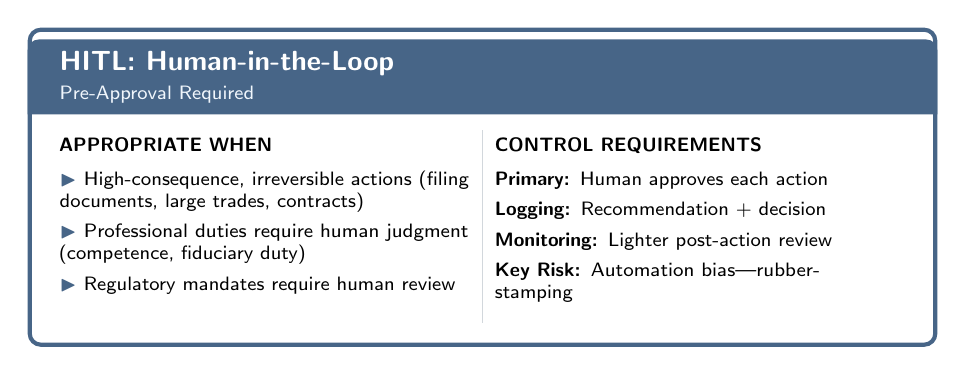
\begin{tikzpicture}[
    every node/.style={inner sep=0pt}
]

% Card frame
\node[
    draw=slate-700,
    line width=1.5pt,
    fill=white,
    minimum width=11.5cm,
    minimum height=4.0cm,
    rounded corners=4pt
] (card) at (0,0) {};

% Header bar
\fill[slate-700, rounded corners=4pt]
    ([yshift=-0.15cm]card.north west) -- ([yshift=-0.15cm]card.north east)
    [rounded corners=0pt] -- ([yshift=-1.1cm]card.north east) -- ([yshift=-1.1cm]card.north west)
    [rounded corners=4pt] -- cycle;

% Level name and tagline
\node[font=\normalsize\bfseries\sffamily, text=white, anchor=west]
    at ([xshift=0.4cm, yshift=-0.45cm]card.north west) {HITL: Human-in-the-Loop};
\node[font=\scriptsize\sffamily, text=slate-100, anchor=west]
    at ([xshift=0.4cm, yshift=-0.85cm]card.north west) {Pre-Approval Required};

% Left column: Appropriate When
\node[
    text width=5.2cm,
    anchor=north west,
    font=\scriptsize\sffamily,
    align=left
] at ([xshift=0.4cm, yshift=-1.4cm]card.north west) {
\textbf{\textsf{APPROPRIATE WHEN}}\\[4pt]
\textcolor{slate-700}{$\blacktriangleright$} High-consequence, irreversible actions (filing documents, large trades, contracts)\\[3pt]
\textcolor{slate-700}{$\blacktriangleright$} Professional duties require human judgment (competence, fiduciary duty)\\[3pt]
\textcolor{slate-700}{$\blacktriangleright$} Regulatory mandates require human review
};

% Vertical divider
\draw[gray-300, line width=0.5pt] ([yshift=-1.3cm]card.north) -- ([yshift=0.3cm]card.south);

% Right column: Control Requirements
\node[
    text width=5.0cm,
    anchor=north west,
    font=\scriptsize\sffamily,
    align=left
] at ([xshift=0.15cm, yshift=-1.4cm]card.north) {
\textbf{\textsf{CONTROL REQUIREMENTS}}\\[4pt]
\textbf{Primary:} Human approves each action\\[3pt]
\textbf{Logging:} Recommendation + decision\\[3pt]
\textbf{Monitoring:} Lighter post-action review\\[3pt]
\textbf{Key Risk:} Automation bias---rubber-stamping
};

\end{tikzpicture}
\end{center}


HITL governance is appropriate when errors carry high consequences and human expertise adds substantial value to decision quality. In legal, financial, and audit contexts, many high-stakes decisions benefit from this mode: the system accelerates research, analysis, or document preparation, but a qualified professional validates the output before it affects clients, counterparties, or regulatory filings. The key governance requirement is ensuring the human review is meaningful—not a rubber stamp—which requires the system to surface sufficient context for informed judgment.

\begin{examplebox}[title={Example: HITL Legal Research}]
A legal research assistant that \emph{iteratively} searches case law: it queries legal databases, evaluates result relevance, refines search terms based on findings, and generates progressive case summaries—all before presenting final output to an attorney for review. The attorney verifies citations, assesses legal reasoning, and takes responsibility for the final work product. \textbf{Note}: If the attorney must approve each individual search query before the next query executes, the system lacks autonomous iteration and is not a full agentic system despite having other properties.
\end{examplebox}

\paragraph{Human-on-the-Loop (HOTL): Monitoring with Intervention}
\glsadd{human-on-the-loop}
In HOTL mode, the system operates autonomously within defined parameters, but humans monitor performance and can intervene if anomalies, errors, or safety concerns arise.

% HOTL Autonomy Specification Card

\begin{center}
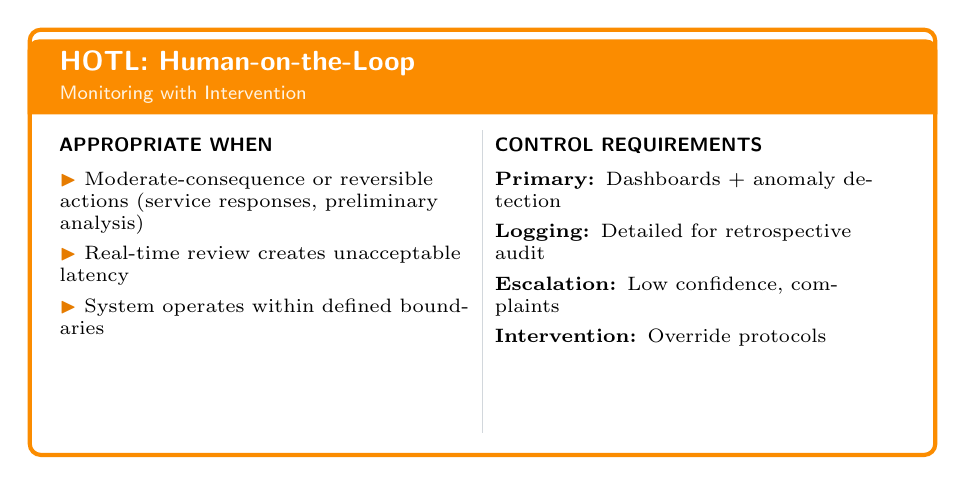
\begin{tikzpicture}[
    every node/.style={inner sep=0pt}
]

% Card frame
\node[
    draw=key-base,
    line width=1.5pt,
    fill=white,
    minimum width=11.5cm,
    minimum height=5.4cm,
    rounded corners=4pt
] (card) at (0,0) {};

% Header bar
\fill[key-base, rounded corners=4pt]
    ([yshift=-0.15cm]card.north west) -- ([yshift=-0.15cm]card.north east)
    [rounded corners=0pt] -- ([yshift=-1.1cm]card.north east) -- ([yshift=-1.1cm]card.north west)
    [rounded corners=4pt] -- cycle;

% Level name and tagline
\node[font=\normalsize\bfseries\sffamily, text=white, anchor=west]
    at ([xshift=0.4cm, yshift=-0.45cm]card.north west) {HOTL: Human-on-the-Loop};
\node[font=\scriptsize\sffamily, text=key-light, anchor=west]
    at ([xshift=0.4cm, yshift=-0.85cm]card.north west) {Monitoring with Intervention};

% Left column: Appropriate When
\node[
    text width=5.2cm,
    anchor=north west,
    font=\scriptsize,
    align=left
] at ([xshift=0.4cm, yshift=-1.4cm]card.north west) {
\textbf{\textsf{APPROPRIATE WHEN}}\\[4pt]
\textcolor{key-dark}{$\blacktriangleright$} Moderate-consequence or reversible actions (service responses, preliminary analysis)\\[3pt]
\textcolor{key-dark}{$\blacktriangleright$} Real-time review creates unacceptable latency\\[3pt]
\textcolor{key-dark}{$\blacktriangleright$} System operates within defined boundaries
};

% Vertical divider
\draw[gray-300, line width=0.5pt] ([yshift=-1.3cm]card.north) -- ([yshift=0.3cm]card.south);

% Right column: Control Requirements
\node[
    text width=5.0cm,
    anchor=north west,
    font=\scriptsize,
    align=left
] at ([xshift=0.15cm, yshift=-1.4cm]card.north) {
\textbf{\textsf{CONTROL REQUIREMENTS}}\\[4pt]
\textbf{Primary:} Dashboards + anomaly detection\\[3pt]
\textbf{Logging:} Detailed for retrospective audit\\[3pt]
\textbf{Escalation:} Low confidence, complaints\\[3pt]
\textbf{Intervention:} Override protocols
};

\end{tikzpicture}
\end{center}


HOTL governance suits situations where transaction volume makes individual review impractical, but errors remain detectable and correctable through monitoring. The system handles routine operations autonomously while humans watch for anomalies—unusual patterns, error spikes, or edge cases that exceed the system's training distribution. Governance focuses on defining clear escalation triggers, maintaining real-time dashboards, and ensuring intervention mechanisms actually work when needed.

\begin{examplebox}[title={Example: HOTL Customer Service}]
A customer service chatbot that handles routine inquiries autonomously but escalates complex questions, complaints, or regulatory issues to human agents. Supervisors monitor conversation logs, error rates, and escalation frequency.
\end{examplebox}

\paragraph{Human-in-Command (HIC): Strategic Oversight and Emergency Stop}
\glsadd{human-in-command}
In HIC mode, the system operates with high autonomy. Humans set strategic goals, define constraints, and monitor aggregate performance but do not review individual decisions. Humans retain emergency stop authority to halt the system if safety violations, systemic failures, or regulatory concerns emerge.

% HIC Autonomy Specification Card

\begin{center}
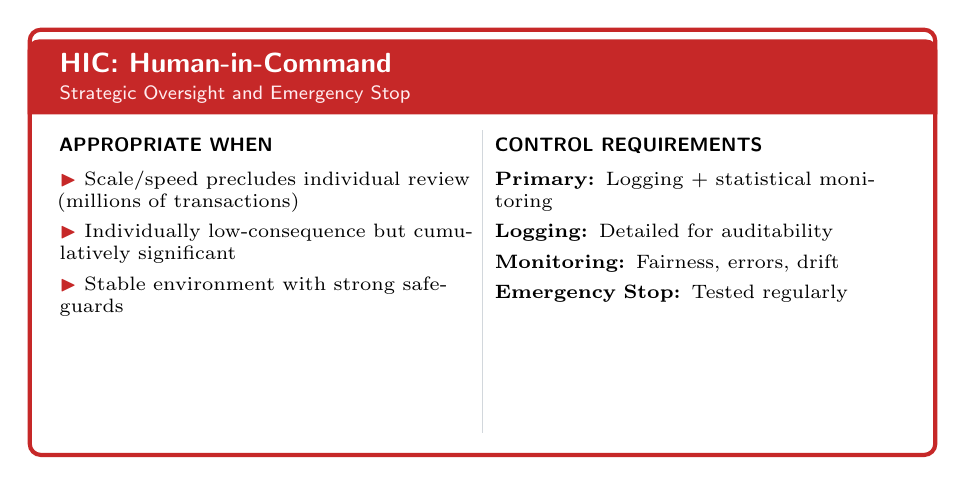
\begin{tikzpicture}[
    every node/.style={inner sep=0pt}
]

% Card frame
\node[
    draw=caution-dark,
    line width=1.5pt,
    fill=white,
    minimum width=11.5cm,
    minimum height=5.4cm,
    rounded corners=4pt
] (card) at (0,0) {};

% Header bar
\fill[caution-dark, rounded corners=4pt]
    ([yshift=-0.15cm]card.north west) -- ([yshift=-0.15cm]card.north east)
    [rounded corners=0pt] -- ([yshift=-1.1cm]card.north east) -- ([yshift=-1.1cm]card.north west)
    [rounded corners=4pt] -- cycle;

% Level name and tagline
\node[font=\normalsize\bfseries\sffamily, text=white, anchor=west]
    at ([xshift=0.4cm, yshift=-0.45cm]card.north west) {HIC: Human-in-Command};
\node[font=\scriptsize\sffamily, text=caution-light, anchor=west]
    at ([xshift=0.4cm, yshift=-0.85cm]card.north west) {Strategic Oversight and Emergency Stop};

% Left column: Appropriate When
\node[
    text width=5.2cm,
    anchor=north west,
    font=\scriptsize,
    align=left
] at ([xshift=0.4cm, yshift=-1.4cm]card.north west) {
\textbf{\textsf{APPROPRIATE WHEN}}\\[4pt]
\textcolor{caution-dark}{$\blacktriangleright$} Scale/speed precludes individual review (millions of transactions)\\[3pt]
\textcolor{caution-dark}{$\blacktriangleright$} Individually low-consequence but cumulatively significant\\[3pt]
\textcolor{caution-dark}{$\blacktriangleright$} Stable environment with strong safeguards
};

% Vertical divider
\draw[gray-300, line width=0.5pt] ([yshift=-1.3cm]card.north) -- ([yshift=0.3cm]card.south);

% Right column: Control Requirements
\node[
    text width=5.0cm,
    anchor=north west,
    font=\scriptsize,
    align=left
] at ([xshift=0.15cm, yshift=-1.4cm]card.north) {
\textbf{\textsf{CONTROL REQUIREMENTS}}\\[4pt]
\textbf{Primary:} Logging + statistical monitoring\\[3pt]
\textbf{Logging:} Detailed for auditability\\[3pt]
\textbf{Monitoring:} Fairness, errors, drift\\[3pt]
\textbf{Emergency Stop:} Tested regularly
};

\end{tikzpicture}
\end{center}


\begin{examplebox}[title={Example: HIC Fraud Detection}]
A credit card fraud detection system that automatically blocks transactions meeting defined risk criteria. Fraud analysts set risk parameters, monitor aggregate block rates and false positive rates, and investigate flagged cases retrospectively. The system can be halted immediately if systemic bias or operational failures are detected.
\end{examplebox}

\paragraph{The Autonomy-Auditability Trade-off}
As summarized in Table~\ref{tab:agents3-autonomy-calibration}, as autonomy increases, the burden of governance shifts from ex-ante (pre-approval) to ex-post (logging, monitoring, audit). HITL systems rely on human review as the primary control; HIC systems rely on comprehensive logging and statistical monitoring. Organizations must invest in monitoring infrastructure proportionate to autonomy: high-autonomy systems cannot rely on ``we'll review it if someone complains.''

\begin{table}[htbp]
\centering
\caption{Autonomy Calibration: Oversight Modes and Control Requirements}
\label{tab:agents3-autonomy-calibration}
\small
\begin{tabular}{>{\raggedright\arraybackslash}p{2.2cm} >{\raggedright\arraybackslash}p{2.8cm} >{\raggedright\arraybackslash}p{2.6cm} >{\raggedright\arraybackslash}p{3.2cm}}
\toprule
\textbf{Autonomy Level} & \textbf{Description} & \textbf{Examples} & \textbf{Controls} \\
\midrule
\textbf{HITL}\newline (Human-in-the-Loop) & Human pre-approves actions & Legal research, investment advice & Approval workflows, bias mitigation \\
\addlinespace
\textbf{HOTL}\newline (Human-on-the-Loop) & Autonomous operation; humans monitor & Customer service, audit analytics & Dashboards, escalation triggers \\
\addlinespace
\textbf{HIC}\newline (Human-in-Command) & High autonomy + emergency stop & Fraud detection, algo trading & Logging, monitoring, fairness metrics \\
\bottomrule
\end{tabular}
\end{table}

\subsection{Entity Frame Calibration}
\label{sec:agents3-entity-frame-calibration}
\glsadd{entity-frame}

Entity frame determines how the system presents itself and how users perceive its role. Entity frame affects trust, liability allocation, and user expectations. Mismatches between entity frame and governance create risk. Table~\ref{tab:agents3-entity-frame-calibration} summarizes entity frame calibration.

\paragraph{Human Entity Frame}
The system represents a specific human professional (e.g., ``your attorney,'' ``your financial adviser''). Users may not distinguish between the professional and the AI tool.

\textbf{Governance implications} establish the highest accountability expectations for human frame systems. Professional responsibility rules apply in full. The professional represented by the system bears liability for all outputs. Confidentiality, competence, and fiduciary duty\glsadd{fiduciary-duty} obligations are non-delegable. Organizations must ensure the professional reviews, validates, and takes ownership of AI-generated outputs.

\textbf{Mismatch risk} arises when the system operates with high autonomy (HIC) but presents a human frame, leading users to assume human oversight that does not exist. This creates misplaced trust and potential liability.

\begin{examplebox}[title={Example: Human Entity Frame}]
A legal research tool that produces work product under the attorney's name. The attorney must verify citations, assess legal reasoning, and ensure compliance with Rule 1.1 (competence) and Rule 3.3 (candor).
\end{examplebox}

\paragraph{Hybrid Entity Frame}
The system is presented as a collaborative partnership between human and AI (e.g., ``AI-assisted analysis,'' ``our team uses advanced tools'').

\textbf{Governance implications} require clear delineation of responsibilities under hybrid frame systems. Users should understand that AI provides preliminary analysis or recommendations, but humans make final decisions. Transparency about the division of labor reduces misplaced trust. Governance must document which tasks are AI-performed vs. human-performed and ensure human review of AI outputs before client-facing use.

\begin{examplebox}[title={Example: Hybrid Entity Frame}]
An investment advisory firm that discloses: ``Our financial plans combine AI-driven market analysis with our advisers' professional judgment and knowledge of your personal circumstances.''
\end{examplebox}

\paragraph{Machine Entity Frame}
The system is clearly identified as a non-human tool (e.g., ``AI chatbot,'' ``automated system''). Users understand they are interacting with technology, not a human.

\textbf{Governance implications} address how machine frame sets appropriate expectations. Users are less likely to assume human judgment, empathy, or professional accountability. Yet organizations must ensure the system's capabilities match user expectations—a chatbot labeled as ``informational only'' should not provide advice that creates reliance. Controls should include clear disclaimers, capability limitations, and escalation to humans for complex or high-stakes issues.

\begin{examplebox}[title={Example: Machine Entity Frame}]
A customer service chatbot that states: ``I'm an AI assistant. I can help with account questions, but for disputes or complex issues, I'll connect you with a human agent.''
\end{examplebox}

\paragraph{Institutional Entity Frame}
The system acts on behalf of the organization (e.g., ``XYZ Bank's credit decisioning system,'' ``our firm's compliance review tool''). The organization, not an individual, bears accountability.

\textbf{Governance implications} show how institutional frame allocates liability to the organization. This is appropriate for systems used in institutional decision-making (credit underwriting, hiring, fraud detection). Governance must include organizational oversight (board and executive accountability), institutional policies (acceptable use, risk appetite), and enterprise-level monitoring. Professional responsibility considerations (if applicable) must be addressed separately.

\textbf{Mismatch risk} emerges when an institutional system operates without adequate organizational oversight (e.g., deployed by a rogue team without executive approval), causing the organization to face liability for decisions it did not authorize.

\begin{examplebox}[title={Example: Institutional Entity Frame}]
A bank's credit pre-screening system that evaluates mortgage applications under institutional policies, with oversight by the Chief Risk Officer and compliance with ECOA.
\end{examplebox}


\begin{table}[htbp]
\centering
\caption{Entity Frame Calibration: Presentation Modes and Accountability Structures}
\label{tab:agents3-entity-frame-calibration}
\small
\begin{tabular}{>{\raggedright\arraybackslash}p{2.0cm} >{\raggedright\arraybackslash}p{2.8cm} >{\raggedright\arraybackslash}p{2.6cm} >{\raggedright\arraybackslash}p{3.4cm}}
\toprule
\textbf{Entity Frame} & \textbf{Description} & \textbf{Examples} & \textbf{Accountability} \\
\midrule
\textbf{Human} & Represents specific professional & Legal research, financial advice & Full professional liability; non-delegable duties \\
\addlinespace
\textbf{Hybrid} & Human-AI collaboration & Audit analytics, co-drafted documents & Shared; human validates AI \\
\addlinespace
\textbf{Machine} & Clearly non-human tool & Chatbot with disclosure & Organization responsible; clear disclaimers \\
\addlinespace
\textbf{Institutional} & Acts for organization & Credit decisions, hiring & Organizational liability; board oversight \\
\bottomrule
\end{tabular}
\end{table}

\subsection{Goal Dynamics Calibration}
\label{sec:agents3-goal-dynamics-calibration}
\glsadd{goal}
\glsadd{goal-dynamics}

Goal dynamics determine how the system's objectives change over time. Static goals are easiest to govern; negotiated goals create the highest misalignment risk. Table~\ref{tab:agents3-goal-dynamics-calibration} summarizes goal dynamics calibration.

\paragraph{Static Goals}
The system pursues a fixed objective defined at deployment. The goal does not change without explicit redeployment.

\textbf{Governance implications} enable static goals to be validated once during pre-deployment review. Organizations assess whether the goal aligns with organizational objectives, legal requirements, and ethical constraints. Once validated, the goal remains stable. Governance focuses on monitoring whether the system achieves the goal and whether side effects emerge.

\begin{examplebox}[title={Example: Static Goals}]
A legal research tool with the static goal: ``Identify cases cited in the brief and verify they exist in official reporters.'' The goal does not change; the tool performs the same validation task repeatedly.
\end{examplebox}

\paragraph{Adaptive Goals}
The system refines its objectives within predefined boundaries based on feedback, but cannot change goals fundamentally. A fraud detection system might adjust risk weights based on observed fraud patterns, yet cannot change its core objective (detect fraud) or operate outside defined risk parameters.

Adaptive goals can drift within their permitted boundaries, and subtle drift may escape notice until it causes harm. Detecting drift requires both a clear standard and active surveillance. The standard comes from explicitly defining which aspects of the goal may adapt and which constraints are inviolable—without this distinction, there is nothing to measure against. Surveillance comes from a monitoring framework that specifies review frequency and revalidation triggers, catching deviation before it compounds. Detection alone is insufficient, however; organizations also need rollback capability, enabling the system to revert to a validated state when adaptation degrades performance or violates constraints.

\begin{examplebox}[title={Example: Adaptive Goals}]
A credit scoring model that adapts feature weights based on performance feedback but cannot introduce new features, change fairness constraints, or operate outside regulatory compliance boundaries.
\end{examplebox}

\paragraph{Negotiated Goals}
When a system proposes changes to its own objectives, every proposal requires human validation before implementation—the system cannot autonomously alter its goals. This creates the highest governance burden of any goal dynamics category. Organizations must designate approval authority, typically reserving this role for senior leadership or a governance committee given the stakes involved. The approval process demands rigorous documentation: why is the system proposing this change, what evidence supports it, and what are the potential consequences? Even after approval, governance is not complete; the modified system must undergo revalidation to confirm it remains safe, fair, and compliant. This cumulative overhead explains why negotiated goals appear only in the most sophisticated agentic deployments.

\begin{examplebox}[title={Example: Negotiated Goals}]
\glsadd{planning}
An AI strategic planning assistant that proposes: ``Based on market analysis, I recommend shifting investment focus from Technology to Healthcare.'' This goal change requires executive approval, risk assessment, and fiduciary duty review.
\end{examplebox}


\begin{table}[htbp]
\centering
\caption{Goal Dynamics Calibration: Objective Stability and Control Requirements}
\label{tab:agents3-goal-dynamics-calibration}
\small
\begin{tabular}{>{\raggedright\arraybackslash}p{2.2cm} >{\raggedright\arraybackslash}p{2.8cm} >{\raggedright\arraybackslash}p{2.6cm} >{\raggedright\arraybackslash}p{3.2cm}}
\toprule
\textbf{Goal Dynamics} & \textbf{Description} & \textbf{Examples} & \textbf{Controls} \\
\midrule
\textbf{Static} & Fixed objectives & Citation verification, compliance checks & One-time validation; monitor side effects \\
\addlinespace
\textbf{Adaptive} & Refinement within boundaries & Credit scoring, fraud detection & Boundaries, monitoring, rollback \\
\addlinespace
\textbf{Negotiated} & System proposes goal changes & Strategic planning, investment strategy & Approval workflows, revalidation \\
\bottomrule
\end{tabular}
\end{table}

\subsection{Persistence Calibration}
\label{sec:agents3-persistence-calibration}
\glsadd{persistence}

Persistence determines whether the system maintains state across interactions. Stateful systems create compounding error risk and require state integrity controls. Table~\ref{tab:agents3-persistence-calibration} summarizes persistence calibration.

\paragraph{Stateless Systems}
Each interaction is independent. The system does not retain information from prior interactions.

\textbf{Governance implications} demonstrate that stateless systems are simpler to govern. Errors do not compound—a mistake in one interaction does not affect subsequent interactions. Logging can be lighter (capture inputs/outputs without state reconstruction). Reproducibility requires only input data, not interaction history.

\begin{examplebox}[title={Example: Stateless System}]
A legal citation verification tool that checks each citation independently. An error in verifying Citation A does not affect the verification of Citation B.
\end{examplebox}

\paragraph{Stateful Systems}
Stateful systems accumulate information across interactions, meaning each decision builds on prior context. This creates a distinctive governance challenge: errors compound. A misunderstanding in one session can propagate through subsequent decisions, corrupting an entire chain of reasoning. Systems require protection of state integrity against tampering, corruption, and adversarial manipulation. Comprehensive logging is essential to enable reconstruction of how state evolved—without it, diagnosing problems becomes nearly impossible. Monitoring must specifically watch for error compounding, catching cases where an early mistake ripples through later decisions. Organizations also need clear criteria for state resets: when should the system discard accumulated context and start fresh? Common triggers include user logout, policy changes, and detected anomalies, though the right criteria depend on deployment context.

\begin{examplebox}[title={Example: Stateful System}]
\glsadd{memory}
A financial planning chatbot that builds a profile of the client's financial situation across multiple conversations. If the system misunderstands the client's risk tolerance in Session 1, all subsequent recommendations may be inappropriate. Governance must include periodic state validation (``Let me confirm: your risk tolerance is Moderate, correct?'') and state logging to reconstruct how the profile evolved.
\end{examplebox}


\begin{table}[htbp]
\centering
\caption{Persistence Calibration: State Management and Control Requirements}
\label{tab:agents3-persistence-calibration}
\small
\begin{tabular}{>{\raggedright\arraybackslash}p{2.2cm} >{\raggedright\arraybackslash}p{2.8cm} >{\raggedright\arraybackslash}p{2.6cm} >{\raggedright\arraybackslash}p{3.2cm}}
\toprule
\textbf{Persistence} & \textbf{Description} & \textbf{Examples} & \textbf{Controls} \\
\midrule
\textbf{Stateless} & Each interaction independent & Citation verification, single queries & Standard logging; errors don't compound \\
\addlinespace
\textbf{Stateful} & State maintained across interactions & Financial planning, fraud monitoring & State integrity, error monitoring, validation \\
\bottomrule
\end{tabular}
\end{table}

\subsection{Integration}
\label{sec:agents3-calibration-integration}
\glsadd{dimensional-calibration}
\glsadd{autonomy-spectrum}
\glsadd{entity-frame}
\glsadd{goal-dynamics}
\glsadd{persistence}

Dimensional calibration becomes powerful when dimensions are integrated. A system's overall risk profile emerges from the \emph{combination} of autonomy, entity frame, goal dynamics, and persistence. Controls must respond to this multidimensional risk.

Table~\ref{tab:agents3-risk-profile-comparison} compares two contrasting risk profiles. The \textbf{low-risk} example is a legal research assistant that verifies whether citations in a brief exist in official reporters and accurately support the propositions for which they are cited. An attorney reviews every output before it reaches a client or court, and each verification stands alone without reference to prior work. The \textbf{high-risk} example is a bank's mortgage underwriting system that evaluates applications, requests documentation, and renders credit decisions. The system learns from outcomes over time, tracks applicant history across multiple interactions, and operates at scale with humans reviewing aggregate performance metrics rather than individual decisions. The low-risk profile demonstrates how strong human oversight compensates for other dimensions, enabling lighter governance. The high-risk profile shows how compounding risk across all four dimensions necessitates intensive controls.

\begin{table}[htbp]
\centering
\caption{Risk Profile Comparison: Low-Risk vs. High-Risk Agentic Systems}
\label{tab:agents3-risk-profile-comparison}
\footnotesize
\begin{tabular}{@{}>{\centering\arraybackslash}p{0.7cm} >{\sffamily\raggedright\arraybackslash}p{1.8cm} >{\raggedright\arraybackslash}p{4.0cm} >{\raggedright\arraybackslash}p{4.0cm}@{}}
\toprule
& & \textbf{Low-Risk: Legal Research} & \textbf{High-Risk: Credit Underwriting} \\
\midrule
\multirow{4}{*}[-1.8em]{\rotatebox[origin=c]{90}{\textbf{Dimension}}}
& Autonomy & HITL—attorney reviews outputs & HIC—autonomous; aggregate monitoring \\
& \cellcolor{bg-neutral}Entity Frame & \cellcolor{bg-neutral}Human—attorney's name & \cellcolor{bg-neutral}Institutional—acts for bank \\
& Goal Dynamics & Static—fixed verification goal & Adaptive—adjusts from feedback \\
& \cellcolor{bg-neutral}Persistence & \cellcolor{bg-neutral}Stateless—independent & \cellcolor{bg-neutral}Stateful—applicant history \\
\midrule
\multirow{7}{*}[-4.5em]{\rotatebox[origin=c]{90}{\textbf{Controls}}}
& Logging & Basic inputs/outputs & Comprehensive—all parameters \\
& \cellcolor{bg-neutral}Monitoring & \cellcolor{bg-neutral}Quarterly spot-checks & \cellcolor{bg-neutral}Continuous fairness, drift \\
& Explainability & Not required & ECOA ``principal reasons'' \\
& \cellcolor{bg-neutral}Fairness & \cellcolor{bg-neutral}Not applicable & \cellcolor{bg-neutral}Pre + continuous + revalidation \\
& Vendor Mgmt & Standard due diligence & Enhanced audit rights \\
& \cellcolor{bg-neutral}Human Oversight & \cellcolor{bg-neutral}Per-output review & \cellcolor{bg-neutral}Monthly/quarterly board \\
& Incident Response & Error correction & Halt; regulator notification \\
\bottomrule
\end{tabular}
\end{table}

\begin{keybox}[title={Dimensional Calibration Worksheet}, breakable=false]
When evaluating a new agentic system, assess each dimension:

\begin{enumerate}
\item \textbf{Autonomy}: HITL, HOTL, or HIC?
\item \textbf{Entity Frame}: Human, Hybrid, Machine, or Institutional?
\item \textbf{Goal Dynamics}: Static, Adaptive, or Negotiated?
\item \textbf{Persistence}: Stateless or Stateful?
\end{enumerate}

Use Tables~\ref{tab:agents3-autonomy-calibration} through \ref{tab:agents3-persistence-calibration} to identify baseline controls for each dimension. Then integrate:
\begin{itemize}
\item High autonomy + institutional frame → Strong logging, statistical monitoring, board oversight.
\item Adaptive goals + stateful persistence → Continuous revalidation, state integrity controls.
\item HITL + human frame → Professional responsibility compliance, automation bias mitigation.
\end{itemize}

Dimensional calibration is not a formula—it is a structured reasoning framework that prevents under-protection (``it's just a chatbot'') and over-engineering (``we must apply maximum controls to everything'').
\end{keybox}

Section~\ref{sec:agents3-implementation} operationalizes dimensional calibration through technical architecture and organizational processes. Section~\ref{sec:agents3-examples} illustrates calibration through worked examples in legal, financial, and audit contexts.



% Section 3: The Governance Stack (Five-Layer Framework)
% ============================================================================
% The Governance Stack---Chapter 3 - How to Govern an Agent
% Purpose: Synthesize regulatory landscape into five-layer framework
% Label: sec:agents3-governance-stack
% ============================================================================

\section{The Governance Stack}
\label{sec:agents3-governance-stack}

With dimensional calibration principles established in Section~\ref{sec:agents3-dimensional}, we now map the overlapping obligations in the regulatory landscape those controls must satisfy. Where Chapter~1 established what agents are and Chapter~2 addressed how to design them, this chapter examines how to govern them in practice. Organizations deploying agentic systems in regulated domains face a complex, overlapping web of legal and professional obligations. There is no single ``AI governance law'' that comprehensively addresses all requirements. Instead, governance emerges from the interaction of five layers: foundational law, professional and ethical obligations, sector-specific regulation, AI-specific regulation, and voluntary governance frameworks. Understanding this layered structure (and why no single layer suffices) is essential for designing governance proportionate to organizational risk.

\subsection{Five-Layer Framework}
\label{sec:agents3-five-layers}

We organize governance obligations into five layers, each building on the foundation below:

\begin{enumerate}
\item \textbf{Foundational Law}: Broadly applicable legal obligations governing data protection, discrimination, consumer protection, and contracts. This layer encompasses not only statutes (such as the General Data Protection Regulation (GDPR), Equal Credit Opportunity Act (ECOA), and state consumer protection statutes) but also tort law as well as other common law principles. Common law doctrines provide protections that predate and operate independently of statutory schemes and include:
\begin{itemize}
\item Defamation law constrains AI-generated content that makes false statements of fact about identifiable individuals.
\item Negligence principles may impose duties of care when deploying systems that foreseeably cause harm.
\item Privacy torts (intrusion upon seclusion, public disclosure of private facts) create liability independent of data protection statutes.
\end{itemize}
These legal foundations establish baselines that apply regardless of whether AI is involved.

\item \textbf{Professional and Ethical Obligations}: Duties imposed on licensed professionals (attorneys, investment advisers, auditors, accountants) by their governing bodies, bar associations, or regulatory agencies. These obligations are often more stringent than general law and impose fiduciary duties, confidentiality requirements, and competence standards.

\item \textbf{Sector-Specific Regulation}: Rules tailored to particular industries (banking, securities, insurance, healthcare) that address operational risks, supervision, and consumer protection in those domains. Examples include Federal Reserve guidance on model risk management (SR 11-7), Financial Industry Regulatory Authority (FINRA) rules on automated systems, and Public Company Accounting Oversight Board (PCAOB) auditing standards.

\item \textbf{AI-Specific Regulation}: Laws and regulations explicitly targeting artificial intelligence systems. The European Union's AI Act is the most comprehensive example, establishing risk-based requirements for high-risk AI systems. U.S. states (Colorado, California, New York City) are enacting their own AI-specific rules addressing bias, transparency, and impact assessments.

\item \textbf{Voluntary Governance Frameworks}: Standards, best practices, and certification schemes developed by standards bodies, industry groups, or government agencies. Examples include the NIST AI Risk Management Framework, ISO/IEC 42001 (AI Management Systems), COBIT for IT governance, and SOC 2 for vendor assurance. These frameworks are typically voluntary unless incorporated by reference into contracts or regulatory requirements.
\end{enumerate}

% Float placement: Change [t!] to [b!] (bottom), [h!] (here), or [htbp] (flexible)
\begin{keybox}[title={Why Layering is Necessary}]
No single framework fully satisfies all governance requirements. The EU AI Act establishes high-level risk categories but does not specify how to comply with ECOA's ``principal reasons'' standard for adverse credit decisions. NIST AI RMF provides flexible risk management guidance but does not address attorney-client privilege or auditor independence. Organizations must layer multiple frameworks, augment them with domain-specific controls, and continuously monitor regulatory developments across jurisdictions.
\end{keybox}

\begin{table}[htbp]
\centering
\small
\begin{tabular}{>{\raggedright\arraybackslash}p{4.0cm} >{\raggedright\arraybackslash}p{3.0cm} >{\raggedright\arraybackslash}p{3.8cm}}
\toprule
\textbf{Layer} & \textbf{Source} & \textbf{Key Examples} \\
\midrule
1. Foundational Law & Statutes, regulations, common law & GDPR, ECOA, tort law \\
\addlinespace
2. Professional Obligations & Bar associations, regulatory bodies & ABA Rules, fiduciary duty, AICPA \\
\addlinespace
3. Sector-Specific Regulation & Industry regulators & SR 11-7, FINRA, PCAOB \\
\addlinespace
4. AI-Specific Regulation & AI-targeted laws & EU AI Act, Colorado AI Act \\
\addlinespace
5. Voluntary Frameworks & Standards bodies & NIST AI RMF, ISO 42001, SOC 2 \\
\bottomrule
\end{tabular}
\caption{Summary of the Five-Layer Governance Framework}
\label{tab:agents3-five-layers}
\end{table}

% Five-Layer Governance Framework - 3D Layer Cake Visualization

\begin{figure}[htbp]
\centering
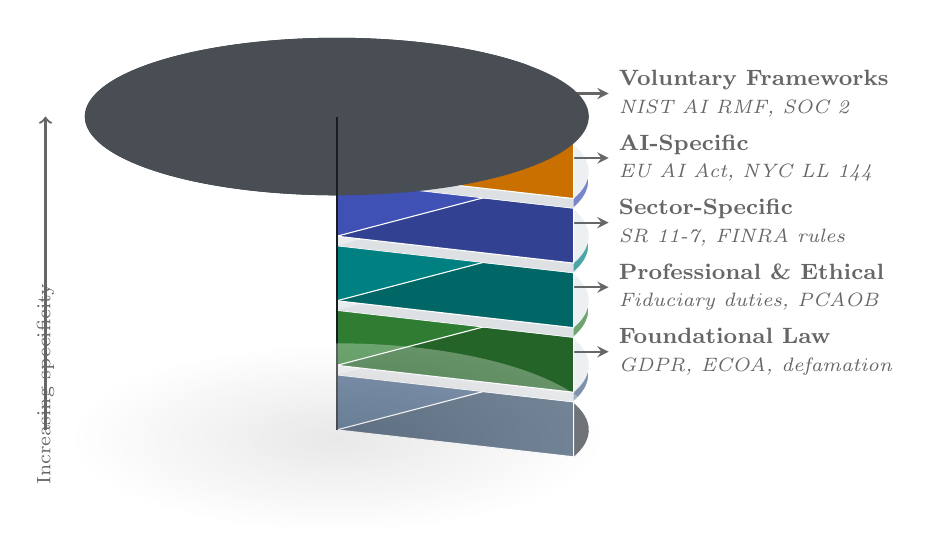
\begin{tikzpicture}[
    label arrow/.style={thick, black!60, ->, >=stealth},
    label text/.style={align=left, anchor=west}
]

% ================= LOCAL COLORS =================
\colorlet{cFoundation}{slate-700}
\colorlet{cProf}{green-900}
\colorlet{cSector}{teal-700}
\colorlet{cAI}{indigo-700}
\colorlet{cVoluntary}{amber-600}
\colorlet{cFrosting}{gray-800}
\colorlet{cFilling}{gray-200}

% ================= CONFIGURATION =================
\def\Rx{3.2}
\def\Ry{1.0}
\def\LayerH{0.7}
\def\FillH{0.12}
\def\CutAngA{-20}
\def\CutAngB{40}

\pgfmathsetmacro{\TotalH}{5*\LayerH + 4*\FillH}

% Pre-calculate edge points on base ellipse
\pgfmathsetmacro{\EdgeRx}{\Rx*cos(\CutAngB)}
\pgfmathsetmacro{\EdgeRy}{\Ry*sin(\CutAngB)}
\pgfmathsetmacro{\EdgeLx}{\Rx*cos(\CutAngA)}
\pgfmathsetmacro{\EdgeLy}{\Ry*sin(\CutAngA)}

% ================= DRAWING =================

% --- 1. BACK SHELL (drawn first, behind everything) ---
% Left wall (from cut edge going back around)
\draw[draw=none, fill=cFrosting]
    (\EdgeLx, \EdgeLy) -- (\EdgeLx, \EdgeLy + \TotalH)
    arc[start angle=\CutAngA, end angle=\CutAngB-360, x radius=\Rx, y radius=\Ry]
    -- (\EdgeRx, \EdgeRy)
    arc[start angle=\CutAngB, end angle=\CutAngA, x radius=\Rx, y radius=\Ry]
    -- cycle;

% --- 2. LAYER 0: Foundational Law ---
\def\yA{0}
% Cut faces (left first, then right - back to front)
\draw[draw=white!50, thin, fill=cFoundation!80!black]
    (0,\yA) -- (\EdgeLx, \EdgeLy + \yA) -- (\EdgeLx, \EdgeLy + \yA + \LayerH) -- (0, \yA + \LayerH) -- cycle;
\draw[draw=white!50, thin, fill=cFoundation]
    (0,\yA) -- (\EdgeRx, \EdgeRy + \yA) -- (\EdgeRx, \EdgeRy + \yA + \LayerH) -- (0, \yA + \LayerH) -- cycle;
% Layer top (ellipse segment)
\pgfmathsetmacro{\yAtop}{\yA + \LayerH}
\draw[draw=white!50, thin, fill=cFoundation!70!white]
    (0, \yAtop) -- (\EdgeRx, \EdgeRy + \yAtop)
    arc[start angle=\CutAngB, end angle=\CutAngA, x radius=\Rx, y radius=\Ry]
    -- cycle;
% Filling layer
\pgfmathsetmacro{\yAf}{\yA + \LayerH}
\draw[draw=none, fill=cFilling!90!gray]
    (0,\yAf) -- (\EdgeLx, \EdgeLy + \yAf) -- (\EdgeLx, \EdgeLy + \yAf + \FillH) -- (0, \yAf + \FillH) -- cycle;
\draw[draw=none, fill=cFilling]
    (0,\yAf) -- (\EdgeRx, \EdgeRy + \yAf) -- (\EdgeRx, \EdgeRy + \yAf + \FillH) -- (0, \yAf + \FillH) -- cycle;
% Filling top
\pgfmathsetmacro{\yAftop}{\yAf + \FillH}
\draw[draw=none, fill=cFilling!80!white]
    (0, \yAftop) -- (\EdgeRx, \EdgeRy + \yAftop)
    arc[start angle=\CutAngB, end angle=\CutAngA, x radius=\Rx, y radius=\Ry]
    -- cycle;
\draw[label arrow] (\EdgeRx, \EdgeRy + \yA + \LayerH/2) -- ++(1.0,0) node[label text] {\footnotesize\textbf{Foundational Law}\\[-2pt]{\scriptsize\textit{GDPR, ECOA, defamation}}};

% --- 3. LAYER 1: Professional & Ethical ---
\pgfmathsetmacro{\yB}{\LayerH + \FillH}
% Cut faces
\draw[draw=white!50, thin, fill=cProf!80!black]
    (0,\yB) -- (\EdgeLx, \EdgeLy + \yB) -- (\EdgeLx, \EdgeLy + \yB + \LayerH) -- (0, \yB + \LayerH) -- cycle;
\draw[draw=white!50, thin, fill=cProf]
    (0,\yB) -- (\EdgeRx, \EdgeRy + \yB) -- (\EdgeRx, \EdgeRy + \yB + \LayerH) -- (0, \yB + \LayerH) -- cycle;
% Layer top
\pgfmathsetmacro{\yBtop}{\yB + \LayerH}
\draw[draw=white!50, thin, fill=cProf!70!white]
    (0, \yBtop) -- (\EdgeRx, \EdgeRy + \yBtop)
    arc[start angle=\CutAngB, end angle=\CutAngA, x radius=\Rx, y radius=\Ry]
    -- cycle;
% Filling layer
\pgfmathsetmacro{\yBf}{\yB + \LayerH}
\draw[draw=none, fill=cFilling!90!gray]
    (0,\yBf) -- (\EdgeLx, \EdgeLy + \yBf) -- (\EdgeLx, \EdgeLy + \yBf + \FillH) -- (0, \yBf + \FillH) -- cycle;
\draw[draw=none, fill=cFilling]
    (0,\yBf) -- (\EdgeRx, \EdgeRy + \yBf) -- (\EdgeRx, \EdgeRy + \yBf + \FillH) -- (0, \yBf + \FillH) -- cycle;
% Filling top
\pgfmathsetmacro{\yBftop}{\yBf + \FillH}
\draw[draw=none, fill=cFilling!80!white]
    (0, \yBftop) -- (\EdgeRx, \EdgeRy + \yBftop)
    arc[start angle=\CutAngB, end angle=\CutAngA, x radius=\Rx, y radius=\Ry]
    -- cycle;
\draw[label arrow] (\EdgeRx, \EdgeRy + \yB + \LayerH/2) -- ++(1.0,0) node[label text] {\footnotesize\textbf{Professional \& Ethical}\\[-2pt]{\scriptsize\textit{Fiduciary duties, PCAOB}}};

% --- 4. LAYER 2: Sector-Specific ---
\pgfmathsetmacro{\yC}{2*(\LayerH + \FillH)}
% Cut faces
\draw[draw=white!50, thin, fill=cSector!80!black]
    (0,\yC) -- (\EdgeLx, \EdgeLy + \yC) -- (\EdgeLx, \EdgeLy + \yC + \LayerH) -- (0, \yC + \LayerH) -- cycle;
\draw[draw=white!50, thin, fill=cSector]
    (0,\yC) -- (\EdgeRx, \EdgeRy + \yC) -- (\EdgeRx, \EdgeRy + \yC + \LayerH) -- (0, \yC + \LayerH) -- cycle;
% Layer top
\pgfmathsetmacro{\yCtop}{\yC + \LayerH}
\draw[draw=white!50, thin, fill=cSector!70!white]
    (0, \yCtop) -- (\EdgeRx, \EdgeRy + \yCtop)
    arc[start angle=\CutAngB, end angle=\CutAngA, x radius=\Rx, y radius=\Ry]
    -- cycle;
% Filling layer
\pgfmathsetmacro{\yCf}{\yC + \LayerH}
\draw[draw=none, fill=cFilling!90!gray]
    (0,\yCf) -- (\EdgeLx, \EdgeLy + \yCf) -- (\EdgeLx, \EdgeLy + \yCf + \FillH) -- (0, \yCf + \FillH) -- cycle;
\draw[draw=none, fill=cFilling]
    (0,\yCf) -- (\EdgeRx, \EdgeRy + \yCf) -- (\EdgeRx, \EdgeRy + \yCf + \FillH) -- (0, \yCf + \FillH) -- cycle;
% Filling top
\pgfmathsetmacro{\yCftop}{\yCf + \FillH}
\draw[draw=none, fill=cFilling!80!white]
    (0, \yCftop) -- (\EdgeRx, \EdgeRy + \yCftop)
    arc[start angle=\CutAngB, end angle=\CutAngA, x radius=\Rx, y radius=\Ry]
    -- cycle;
\draw[label arrow] (\EdgeRx, \EdgeRy + \yC + \LayerH/2) -- ++(1.0,0) node[label text] {\footnotesize\textbf{Sector-Specific}\\[-2pt]{\scriptsize\textit{SR 11-7, FINRA rules}}};

% --- 5. LAYER 3: AI-Specific ---
\pgfmathsetmacro{\yD}{3*(\LayerH + \FillH)}
% Cut faces
\draw[draw=white!50, thin, fill=cAI!80!black]
    (0,\yD) -- (\EdgeLx, \EdgeLy + \yD) -- (\EdgeLx, \EdgeLy + \yD + \LayerH) -- (0, \yD + \LayerH) -- cycle;
\draw[draw=white!50, thin, fill=cAI]
    (0,\yD) -- (\EdgeRx, \EdgeRy + \yD) -- (\EdgeRx, \EdgeRy + \yD + \LayerH) -- (0, \yD + \LayerH) -- cycle;
% Layer top
\pgfmathsetmacro{\yDtop}{\yD + \LayerH}
\draw[draw=white!50, thin, fill=cAI!70!white]
    (0, \yDtop) -- (\EdgeRx, \EdgeRy + \yDtop)
    arc[start angle=\CutAngB, end angle=\CutAngA, x radius=\Rx, y radius=\Ry]
    -- cycle;
% Filling layer
\pgfmathsetmacro{\yDf}{\yD + \LayerH}
\draw[draw=none, fill=cFilling!90!gray]
    (0,\yDf) -- (\EdgeLx, \EdgeLy + \yDf) -- (\EdgeLx, \EdgeLy + \yDf + \FillH) -- (0, \yDf + \FillH) -- cycle;
\draw[draw=none, fill=cFilling]
    (0,\yDf) -- (\EdgeRx, \EdgeRy + \yDf) -- (\EdgeRx, \EdgeRy + \yDf + \FillH) -- (0, \yDf + \FillH) -- cycle;
% Filling top
\pgfmathsetmacro{\yDftop}{\yDf + \FillH}
\draw[draw=none, fill=cFilling!80!white]
    (0, \yDftop) -- (\EdgeRx, \EdgeRy + \yDftop)
    arc[start angle=\CutAngB, end angle=\CutAngA, x radius=\Rx, y radius=\Ry]
    -- cycle;
\draw[label arrow] (\EdgeRx, \EdgeRy + \yD + \LayerH/2) -- ++(1.0,0) node[label text] {\footnotesize\textbf{AI-Specific}\\[-2pt]{\scriptsize\textit{EU AI Act, NYC LL 144}}};

% --- 6. LAYER 4: Voluntary Frameworks ---
\pgfmathsetmacro{\yE}{4*(\LayerH + \FillH)}
% Cut faces
\draw[draw=white!50, thin, fill=cVoluntary!80!black]
    (0,\yE) -- (\EdgeLx, \EdgeLy + \yE) -- (\EdgeLx, \EdgeLy + \yE + \LayerH) -- (0, \yE + \LayerH) -- cycle;
\draw[draw=white!50, thin, fill=cVoluntary]
    (0,\yE) -- (\EdgeRx, \EdgeRy + \yE) -- (\EdgeRx, \EdgeRy + \yE + \LayerH) -- (0, \yE + \LayerH) -- cycle;
% Layer top (this becomes the lid, drawn later)
\draw[label arrow] (\EdgeRx, \EdgeRy + \yE + \LayerH/2) -- ++(1.0,0) node[label text] {\footnotesize\textbf{Voluntary Frameworks}\\[-2pt]{\scriptsize\textit{NIST AI RMF, SOC 2}}};

% --- 7. TOP LID (shifted up to top of cake) ---
\begin{scope}[yshift=\TotalH cm]
\draw[draw=none, fill=cFrosting!90!white]
    (0,0) -- (\EdgeRx, \EdgeRy)
    arc[start angle=\CutAngB, end angle=\CutAngA-360, x radius=\Rx, y radius=\Ry]
    -- cycle;
\end{scope}

% --- 8. FINISHES ---
\draw[thick, cFrosting!50!black] (0,0) -- (0,\TotalH);

\shade[inner color=black!30, outer color=white, opacity=0.3]
    (0,-0.1) ellipse ({\Rx+0.2} and {\Ry+0.2});

\draw[->, thick, black!60] ({-\Rx-0.5}, 0) -- ({-\Rx-0.5}, \TotalH)
    node[midway, left, rotate=90] {\scriptsize Increasing specificity};

\end{tikzpicture}
\caption{The five-layer governance framework visualized as stacked obligations. Each layer builds on the foundation below: foundational law (statutes and common law) provides the broadest baseline; professional duties add licensed-practice requirements; sector-specific rules address industry contexts; AI-specific regulation targets algorithmic systems directly; and voluntary frameworks offer certification and best-practice guidance. Organizations must address all applicable layers---no single layer provides complete coverage.}
\label{fig:agents3-five-layer-framework}
\end{figure}


The remainder of this section examines each layer in detail, identifying key requirements and illustrating how obligations interact.

\subsection{Layer 1: Foundational Law}
\label{sec:agents3-foundational-law}

Foundational law provides the baseline for governance, applicable to all organizations regardless of industry or use case. Three domains are especially relevant:

\paragraph{Data Protection and Privacy: GDPR Article 22 and Stateful Agentic Systems}
The GDPR establishes rights and obligations for processing personal data of EU residents. Article 22 addresses automated decision-making: individuals have the right not to be subject to decisions based solely on automated processing that produce legal or similarly significant effects \parencite{gdpr-article-22}. While not an absolute prohibition (automated decisions are permitted with explicit consent, contractual necessity, or legal authorization), Article 22 requires organizations to implement ``suitable measures'' to safeguard the data subject's rights, including the right to obtain human intervention and contest the decision.

\textbf{Agentic-Specific Challenge: Stateful Decision Accumulation}: Article 22's human intervention requirement becomes complex for stateful agentic systems that accumulate context across multiple cycles. Generic AI guidance suggests ``add a button for human review,'' but this is insufficient for agentic systems. Building on Chapter~1's analysis of iteration and adaptation, meaningful human intervention requires access to the system's accumulated internal state: how the agent's understanding evolved across iterations, what adaptations occurred, and what termination logic triggered the final decision. Without comprehensive state logging (capturing perception, action, and rationale at each cycle), human reviewers cannot meaningfully intervene or contest decisions because they lack visibility into how the agent reached its conclusion.

\emph{Governance Implication}: For agentic systems subject to GDPR Article 22, human intervention controls must be paired with state logging requirements (cross-cycle audit trails). Organizations cannot satisfy Article 22 by providing post-hoc review without the ability to reconstruct the agent's iterative decision process. This links directly to the State Logging control discussed in Section~\ref{sec:agents3-audit-logging}.

Article 32 requires appropriate technical and organizational security measures, including encryption, pseudonymization, and resilience against unauthorized processing. Articles 33-34 mandate breach notification to supervisory authorities (within 72 hours) and affected individuals (without undue delay) when breaches pose risks to rights and freedoms.

For organizations operating globally, GDPR compliance often sets the de facto standard. Even organizations without EU operations may face GDPR obligations if they offer services to EU residents or monitor their behavior.

\paragraph{Anti-Discrimination and Fair Lending: ECOA and Process-Based Discrimination}
The Equal Credit Opportunity Act (ECOA) prohibits credit discrimination based on race, color, religion, national origin, sex, marital status, age, or receipt of public assistance \parencite{ecoa}. Regulation B, which implements ECOA, requires creditors to provide ``principal reasons'' for adverse credit decisions \parencite{ecoa-reg-b}. This explainability requirement is more specific than generic AI transparency guidance; applicants must receive concrete, understandable reasons tied to the factors that most significantly influenced the decision.

ECOA applies regardless of whether the decision was made by a human, an algorithm, or a hybrid system. Courts have applied \emph{disparate impact} theory: even facially neutral criteria can violate ECOA if they disproportionately harm protected classes without adequate business justification.

\textbf{Agentic-Specific Challenge: Process-Based Discrimination}: Traditional fairness testing focuses on \emph{outcome parity} (do protected classes receive approvals at comparable rates?). For agentic credit underwriting systems that iteratively investigate applications across multiple cycles, discrimination can emerge through the \emph{investigation process} itself, not just final decisions. An agentic system might:
\begin{itemize}
\item Adapt to request more verification cycles from applicants with characteristics correlated with protected classes (e.g., shorter U.S. employment tenure as a proxy for national origin).
\item Impose higher process burdens (more documentation requests, longer investigation timelines) on protected groups, causing application abandonment even if the system would ultimately approve.
\item Learn patterns that create disparate \emph{iteration counts} across demographic groups, violating ECOA even when final approval rates satisfy the 80\% rule commonly used in disparate impact analysis.
\end{itemize}

\emph{Governance Implication}: Agentic credit systems require \emph{process parity monitoring} in addition to outcome fairness testing. Organizations must audit:
\begin{itemize}
\item Average investigation cycles by protected class (flag if deviation >20\%).
\item Termination reasons by demographic group (ensure similar rates of confidence-based vs. timeout-based termination).
\item Application abandonment rates during multi-cycle investigation (ensure verification burdens do not disproportionately affect protected classes).
\end{itemize}

Systems require controls ensuring that dynamic investigation strategies do not introduce prohibited discrimination, a challenge that does not arise with single-shot credit scoring models. See Section~\ref{sec:agents3-monitoring-incident} for a worked example of process-based discrimination detected in agentic underwriting.

\paragraph{Consumer Protection}
State consumer protection statutes (e.g., Unfair and Deceptive Acts and Practices laws) prohibit misleading representations and unfair business practices. If an AI chatbot misrepresents its capabilities, provides inaccurate information, or fails to disclose material limitations, the organization may face consumer protection enforcement regardless of whether the misrepresentation was intentional or the result of a model hallucination.

\subsection{Layer 2: Professional and Ethical Obligations}
\label{sec:agents3-professional-obligations}

Licensed professionals face heightened obligations that governance systems must operationalize. We examine three domains:

\paragraph{Legal Practice: ABA Model Rules}
Most U.S. jurisdictions have adopted versions of the American Bar Association's Model Rules of Professional Conduct. Three rules are especially salient for AI governance:

\begin{itemize}
\item \textbf{Rule 1.1 (Competence)}: An attorney must provide competent representation, requiring ``the legal knowledge, skill, thoroughness and preparation reasonably necessary for the representation.'' ABA Formal Opinion 512 (July 2024) clarifies that competence includes understanding AI tools' capabilities and limitations \parencite{aba-formal-opinion-512}; attorneys cannot delegate legal analysis to AI without independent verification.

\item \textbf{Rule 1.6 (Confidentiality)}: An attorney must not reveal information relating to representation of a client unless the client gives informed consent. Using AI tools that transmit client data to third-party vendors, train models on client information, or store data insecurely may violate confidentiality obligations. Organizations must assess vendor data handling practices and obtain client consent where necessary.

\item \textbf{Rule 3.3 (Candor Toward the Tribunal)}: An attorney must not knowingly make false statements of fact or law to a tribunal. Submitting AI-generated legal research without verification can result in fabricated citations or misrepresented holdings, which violates this duty. Courts have imposed sanctions ranging from \$1,000 to \$15,000 for such violations, with some attorneys facing suspension or mandatory disclosure requirements on future filings.
\end{itemize}

Rule 5.3 addresses supervision of nonlawyer assistants, a framework some jurisdictions apply to AI tools. The attorney remains responsible for ensuring that AI-assisted work product meets professional standards.

\paragraph{Financial Services: Fiduciary Duty and Suitability}
\glsadd{fiduciary-duty}Investment advisers owe fiduciary duties to clients under the Investment Advisers Act of 1940 and SEC interpretations. This duty has two components:

\begin{itemize}
\item \textbf{Duty of Care}: Providing advice that is suitable for the client's financial situation, investment objectives, and risk tolerance. An AI-generated portfolio recommendation must be validated against these client-specific factors.

\item \textbf{Duty of Loyalty}: Acting in the client's best interest, including full disclosure of conflicts of interest. If an AI tool is provided by an affiliate, receives compensation from recommended products, or prioritizes firm profitability over client outcomes, the adviser must disclose these conflicts and ensure recommendations remain in the client's best interest.
\end{itemize}

FINRA (Financial Industry Regulatory Authority) Rule 2111 imposes a similar suitability obligation on broker-dealers. Rule 3110 requires firms to supervise associated persons and establish procedures to ensure compliance. For AI systems that generate investment recommendations or execute trades, governance must include supervisory review procedures, monitoring for suitability violations, and escalation protocols.

\paragraph{Audit and Accounting: Independence and Skepticism}
The AICPA Code of Professional Conduct and PCAOB auditing standards impose strict independence and competence requirements on auditors:

\begin{itemize}
\item \textbf{Independence}: Auditors must maintain both independence in fact and independence in appearance. If an AI tool is provided by the audit client, an affiliate, or a vendor with financial ties to the client, independence may be impaired; the SEC and PCAOB closely scrutinize auditor-provided tools that could create management decision-making or self-review threats.

\item \textbf{Professional Skepticism}: PCAOB Auditing Standard 1015 requires auditors to exercise professional skepticism: a questioning mind and critical assessment of audit evidence. Auditors cannot accept AI outputs uncritically; they must understand the tool's methodology, validate its logic, and assess whether results are consistent with other evidence.

\item \textbf{Documentation}: AS 1215 (Audit Documentation) requires auditors to document the nature, timing, extent, and results of audit procedures. If AI is used for sampling, risk assessment, or analytical procedures, the workpapers must explain the tool's logic, parameters, and the auditor's rationale for relying on its output \parencite{pcaob-as1215}.
\end{itemize}

These professional obligations are non-delegable. Governance systems must operationalize competence, confidentiality, independence, and documentation requirements through technical controls and organizational processes.

\subsection{Layer 3: Sector-Specific Regulation}
\label{sec:agents3-sector-regulation}

Sector regulators impose industry-tailored requirements that general frameworks do not address:

\paragraph{Banking: Model Risk Management}
The Federal Reserve, Office of the Comptroller of the Currency (OCC), and Federal Deposit Insurance Corporation (FDIC) issued SR 11-7 on model risk management \parencite{fed-sr11-7}. SR 11-7 applies broadly to model risk management in banking. Key requirements include:

\begin{itemize}
\item \textbf{Model Inventory}: Maintain a comprehensive inventory of models, classified by risk.
\item \textbf{Independent Validation}: Models must be validated by a function independent of the model's development and use. Validation includes conceptual soundness review, ongoing monitoring, and outcomes analysis.
\item \textbf{Model Governance}: Establish board and senior management oversight, clear roles and responsibilities, and policies for model development, implementation, and use.
\item \textbf{Documentation}: Maintain complete documentation of model logic, data sources, assumptions, limitations, and validation.
\end{itemize}

\textbf{Application to Agentic Systems}: For agentic systems deployed in banking (e.g., iterative credit underwriting agents that gather information across multiple cycles, adapt criteria based on discovered patterns, and escalate edge cases), SR 11-7 requires documentation of all six operational properties. Unlike traditional one-shot credit models that execute fixed logic, agentic systems must document iteration logic (when does the system gather more data?), adaptation mechanisms (how do criteria evolve?), and termination conditions (when does it escalate to humans?).

\paragraph{Securities: FINRA Supervision and Algorithmic Trading}
FINRA Rule 3110 requires broker-dealers to establish supervisory systems reasonably designed to achieve compliance with applicable laws and regulations. For firms using algorithmic trading systems or AI-driven investment recommendations, this means:

\begin{itemize}
\item \textbf{Pre-Deployment Testing}: Validate algorithms in a controlled environment before production use.
\item \textbf{Ongoing Monitoring}: Continuously monitor for erroneous or manipulative behavior.
\item \textbf{Risk Controls}: Implement automated controls (e.g., price collars, volume limits) to prevent runaway algorithms.
\item \textbf{Supervisory Review}: Designate supervisors responsible for algorithm oversight and establish escalation procedures.
\end{itemize}

\paragraph{Audit: PCAOB Standards on Audit Evidence and Sampling}
The PCAOB has not issued AI-specific guidance, but existing auditing standards apply. AS 1105 (Audit Evidence) establishes that the auditor is responsible for all audit evidence, regardless of source.

\textbf{Application to Agentic Systems}: For agentic audit systems (e.g., agents that iteratively refine sampling strategies based on discovered anomalies, adapt risk assessments as they review documentation, and terminate when coverage objectives are met), PCAOB standards require:

\begin{itemize}
\item Documentation of iteration logic: How does the system refine its sampling or analysis strategy across cycles?
\item Documentation of adaptation mechanisms: When and why does the system adjust risk assessments or expand sample sizes?
\item Documentation of termination criteria: What triggers the system to conclude its work or escalate to human auditors?
\item Understanding the tool's methodology and assumptions across all six GPA+IAT properties.
\item Professional skepticism maintained throughout; auditors cannot delegate professional judgment to autonomous systems.
\end{itemize}

AS 2315 (Audit Sampling) requires auditors to design samples that provide a reasonable basis for conclusions. Agentic sampling systems must document how iteration and adaptation enhance (rather than compromise) statistical validity.

\subsection{Layer 4: AI-Specific Regulation}
\label{sec:agents3-ai-regulation}

AI-specific regulation is emerging rapidly. We focus on the most comprehensive framework and notable U.S. developments:

\paragraph{EU AI Act: Risk-Based Tiering}
The EU AI Act, which entered into force in August 2024, establishes a risk-based regulatory framework \parencite{eu-ai-act-2024}:

\begin{itemize}
\item \textbf{Prohibited Practices}: AI systems that pose unacceptable risks (e.g., social scoring by governments, real-time biometric identification in public spaces except narrow law enforcement exceptions, manipulative or harmful systems) are banned.

\item \textbf{High-Risk Systems}: AI systems used in employment, education, credit assessment, law enforcement, critical infrastructure, and biometric identification are classified as high-risk. These systems must satisfy stringent requirements:
  \begin{itemize}
  \item \textbf{Risk Management} (Article 9): Establish and maintain a risk management system throughout the AI system's lifecycle.
  \item \textbf{Data Governance} (Article 10): Training, validation, and testing datasets must be relevant, representative, and free from bias to the extent possible.
  \item \textbf{Logging} (Article 12): Maintain automatic recording of events (logs) to enable traceability.
  \item \textbf{Transparency} (Article 13): Provide clear instructions for use, including capabilities, limitations, and expected performance.
  \item \textbf{Human Oversight} (Article 14): Design systems to enable effective oversight, including the ability to override or interrupt the system.
  \item \textbf{Accuracy, Robustness, Cybersecurity} (Article 15): Achieve appropriate levels of accuracy and resilience against errors, faults, and cyberattacks.
  \item \textbf{Conformity Assessment} (Article 43): High-risk systems must undergo third-party conformity assessment before market placement (for certain categories) or internal assessment (for others).
  \end{itemize}

\item \textbf{Limited-Risk and Minimal-Risk Systems}: Lower-risk systems face transparency obligations (e.g., chatbots must disclose they are AI) but not the full high-risk requirements.
\end{itemize}

Penalties for non-compliance are severe: up to €35~million or 7\% of global annual turnover for prohibited practices, and up to €15~million or 3\% for high-risk system violations. Organizations operating in or serving EU markets must assess whether their agentic systems fall within high-risk categories and implement Article 9--15 requirements.

\paragraph{U.S. State and Local AI Laws}
In the absence of comprehensive federal AI legislation, U.S. states and cities are enacting targeted rules:

\begin{itemize}
\item \textbf{Colorado AI Act (SB 24-205)}: Effective January 1, 2026, Colorado's law prohibits algorithmic discrimination: deployment of high-risk AI systems that result in unlawful differential treatment or impact based on protected classifications \parencite{colorado-ai-act}. Deployers must conduct impact assessments documenting the system's purpose, data sources, intended benefits, known limitations, and measures to mitigate discrimination. A rebuttable presumption of compliance applies if deployers complete a reasonable impact assessment in good faith.

\item \textbf{New York City Local Law 144 (Automated Employment Decision Tools)}: Effective since July 2023, NYC requires employers using AI for hiring or promotion to conduct annual bias audits, publish summary results, and notify candidates that an automated tool is in use. Employers must also allow candidates to request alternative evaluation processes.

\item \textbf{California Privacy Rights Act (CPRA) and Proposed AI Legislation}: California has enacted data protection laws that indirectly regulate AI (e.g., CPRA's provisions on automated decision-making) and is considering comprehensive AI legislation addressing high-risk uses.
\end{itemize}

These patchwork requirements mean organizations must track regulatory developments across jurisdictions and tailor governance to the most stringent applicable standard.

\subsection{Layer 5: Voluntary Governance Frameworks}
\label{sec:agents3-frameworks}

Voluntary frameworks provide structured approaches to AI governance. Organizations often adopt multiple frameworks to address different audiences and objectives:

\paragraph{NIST AI Risk Management Framework (AI RMF 1.0)}
Published in January 2023, the NIST AI RMF is a flexible, voluntary framework for managing AI risks \parencite{nist-ai-rmf}. It organizes activities into four functions:

\begin{itemize}
\item \textbf{Govern}: Establish organizational structures, policies, and accountability for AI risk management.
\item \textbf{Map}: Identify context, stakeholders, and potential impacts of AI systems.
\item \textbf{Measure}: Assess and benchmark AI system performance, including trustworthiness characteristics (fairness, transparency, accountability, safety, privacy, security).
\item \textbf{Manage}: Allocate resources, implement risk treatments, and monitor effectiveness.
\end{itemize}

NIST AI RMF emphasizes trustworthiness characteristics and provides flexibility for organizations of different sizes and sectors. It is widely referenced by federal agencies, state regulators, and private-sector organizations as a baseline governance framework.

\paragraph{ISO/IEC 42001:2023 (AI Management Systems)}
ISO/IEC 42001 is an international standard for AI management systems, providing a certifiable framework \parencite{iso-iec-42001}. It establishes requirements for establishing, implementing, maintaining, and continually improving an AI management system. Annex A provides 40+ AI-specific controls organized by category (data management, model development, deployment, monitoring).

ISO/IEC 42001 is especially relevant for organizations:
\begin{itemize}
\item Operating in EU markets (the standard is recognized as supporting EU AI Act compliance).
\item Seeking third-party certification to demonstrate governance maturity.
\item Requiring international recognition (ISO standards are globally accepted).
\end{itemize}

Certification typically costs \$50,000--\$150,000 and requires 3--6 months, depending on organizational size and maturity.

\paragraph{COBIT (IT Governance Framework)}
COBIT, developed by ISACA, is a comprehensive IT governance framework widely used by enterprises. COBIT 2019 includes guidance on emerging technologies, including AI. Organizations with mature IT governance often extend COBIT to cover AI systems rather than creating parallel structures.

COBIT is best suited for organizations seeking to integrate AI governance into existing enterprise IT governance rather than treating AI as a standalone domain.

\paragraph{SOC 2 Type II (Vendor Assurance)}
SOC 2 (Service Organization Control) is an auditing framework for service providers, especially SaaS vendors. SOC 2 Type II reports assess controls over security, availability, processing integrity, confidentiality, and privacy over a period of time (typically 6--12 months).

For organizations procuring AI tools from vendors, a SOC 2 Type II report provides independent assurance that the vendor has implemented and operated controls effectively. Many enterprises require SOC 2 reports as a condition of vendor contracts.

\paragraph{Framework Selection Logic}
Organizations often layer frameworks:

\begin{itemize}
\item \textbf{Start with NIST AI RMF} for flexible internal governance (free, widely recognized, no certification requirement).
\item \textbf{Add ISO/IEC 42001} if seeking certification, operating in EU markets, or facing customer demands for third-party assurance.
\item \textbf{Integrate with COBIT} if mature IT governance structures exist.
\item \textbf{Require SOC 2} from third-party AI vendors to validate their controls.
\end{itemize}

No single framework addresses all requirements. Layering enables organizations to satisfy general governance needs (NIST), achieve certification (ISO), integrate with enterprise governance (COBIT), and validate vendor controls (SOC 2).

\subsection{Seven Common Controls Across Frameworks}
\label{sec:agents3-common-controls}

Despite structural differences, all governance frameworks converge on seven common controls:

\begin{enumerate}
\item \textbf{Risk Assessment and Management}: Identify, assess, prioritize, and mitigate AI-related risks throughout the system lifecycle. Risk assessment is the foundation for all subsequent governance activities.

\item \textbf{Human Oversight}: Implement oversight mechanisms proportionate to system autonomy and risk: human-in-the-loop (pre-approval for high-stakes decisions), human-on-the-loop (monitoring with intervention capability), or human-in-command (strategic oversight with emergency stop authority).

\item \textbf{Audit Logging and Traceability}: Maintain tamper-evident logs that capture inputs, outputs, decisions, and human interventions. Logs must enable reconstruction of decisions for audit, investigation, and regulatory review.

\item \textbf{Explainability and Transparency}: Provide stakeholders (users, auditors, regulators) with understandable information about how the system operates, what factors influence decisions, and what limitations exist. Explainability techniques must be validated for faithfulness (reflects actual model logic), completeness (material factors included), and usefulness (enables informed decisions).

\item \textbf{Vendor Management}: Assess, monitor, and manage third-party AI vendors. Vendor due diligence, contract negotiation, ongoing monitoring, and escalation procedures are essential because vendor risks cascade into organizational liability.

\item \textbf{Incident Response and Remediation}: Detect, triage, contain, investigate, remediate, and learn from AI system failures. Incident response must be rapid (fairness violations and safety failures require immediate action) and systematic (root cause analysis, notification, continuous improvement).

\item \textbf{Documentation and Record-Keeping}: Maintain comprehensive documentation of system purpose, design, data sources, validation results, deployment decisions, monitoring outputs, and incidents. Documentation supports audits, regulatory inquiries, and continuous improvement.
\end{enumerate}

While frameworks differ in emphasis and structure, these seven controls represent governance universals. Section~\ref{sec:agents3-dimensional} (presented earlier) established how to calibrate control intensity based on system properties. Section~\ref{sec:agents3-implementation} operationalizes these calibrated controls through technical architecture and organizational processes.



% Section 4: Implementation (Building Governance Systems)
% ============================================================================
% Implementation: Building Governance Systems — Chapter 3 - How to Govern an Agent
% Purpose: Operationalize governance through controls and processes
% Label: sec:agents3-implementation
% ============================================================================

\section{Implementation}
\label{sec:agents3-implementation}

Section~\ref{sec:agents3-dimensional} established principles for calibrating control intensity. We now focus on building governance systems by operationalizing those principles. We now turn to operationalizing those principles: how to design and implement risk assessment, audit logging, explainability, human oversight, vendor management, performance monitoring, and incident response. Where Chapter~2 established the technical infrastructure for logging, escalation, and action controls, we now address the governance policies and organizational processes that make those capabilities enforceable. We focus on actionable guidance—what practitioners and governance teams actually build—illustrated through examples from legal, financial, and audit domains.

\subsection{Risk Assessment}
\label{sec:agents3-risk-assessment}

All governance begins with risk assessment. Before deploying an agentic system, organizations must systematically identify harm scenarios, assess their likelihood and impact, document mitigations, and define reassessment triggers.

\paragraph{Risk Assessment Methodology}
Effective risk assessment addresses six categories of AI-related harms:

\begin{itemize}
\item \textbf{Bias and Fairness}: Does the system produce discriminatory outcomes? Are protected classes disproportionately harmed?
\item \textbf{Accuracy and Reliability}: Does the system produce correct outputs? What is the error rate? What are the consequences of errors?
\item \textbf{Security}: Can adversaries manipulate inputs (prompt injection), poison training data, or exfiltrate sensitive information?
\item \textbf{Privacy}: Does the system access, process, or disclose personal or confidential information inappropriately?
\item \textbf{Safety}: Can system failures cause physical harm, financial loss, or operational disruption?
\item \textbf{Compliance}: Does deployment violate laws, regulations, or professional obligations?
\end{itemize}

For each risk category, assess \emph{likelihood} (how probable is this harm?), \emph{impact} (if it occurs, how severe are the consequences?), \emph{affected stakeholders} (who is harmed?), and \emph{mitigations} (what controls reduce risk?). Document \emph{residual risk} after mitigations and obtain approval from appropriate governance authority (e.g., risk committee, general counsel, board for high-risk systems).

Define \emph{reassessment triggers}: When must the risk assessment be updated? Common triggers include model updates, policy changes, regulatory developments, incident discoveries, and significant drift in performance or fairness metrics.

\paragraph{Example: Agentic Financial Planning Assistant Risk Assessment}
\glsadd{escalation}\glsadd{planning}
A registered investment adviser deploys an agentic financial planning system that \emph{iteratively} analyzes client portfolios, adapts recommendations based on market conditions and client feedback, and determines when to escalate to human advisers.

The system iterates through analysis-recommendation-feedback loops over days or weeks, adapts its strategy based on client responses and market changes, and terminates when confidence thresholds are met or escalation is required. As Chapter~2 established, these iteration, adaptation, and termination capabilities create governance requirements beyond simple AI tools. \textit{Dimensional profile: HITL + hybrid frame + adaptive goals + stateful.}

The risk assessment identifies five primary concerns, summarized in Table~\ref{tab:agents3-financial-planning-risk}.

\emph{Compliance risk} ranks highest: the system may recommend unsuitable investments, violating Advisers Act fiduciary duty. Unlike a simple Q\&A chatbot, iteration and adaptation create compounding risk—a flawed recommendation in cycle one shapes subsequent analysis.

\glsadd{hallucination}\emph{Accuracy risk} stems from potential hallucination of market data or misinterpretation of client constraints. Across iterative cycles, these errors compound rather than self-correct.

\emph{Adaptation risk} arises when the system drifts from regulatory compliance—as an instance, learning to recommend higher-fee products based on firm incentives rather than client best interest.

\emph{Iteration risk} manifests as either excessive iteration (analysis paralysis) or premature termination (incomplete analysis).

\emph{Security risk}, though less likely, carries the highest impact: prompt injection across iterative cycles could manipulate accumulated state, potentially disclosing other clients' information.

\begin{table}[htbp]
\centering
\caption[Risk Assessment: Agentic Financial Planning Assistant]{Risk Assessment: Agentic Financial Planning Assistant. Risk levels: \protect\tikz[baseline=-0.5ex]\protect\draw[fill=red-900,draw=none] (0,0) circle (0.35em); Critical, \protect\tikz[baseline=-0.5ex]\protect\draw[fill=red-600,draw=none] (0,0) circle (0.35em); High, \protect\tikz[baseline=-0.5ex]\protect\draw[fill=amber-600,draw=none] (0,0) circle (0.35em); Moderate, \protect\tikz[baseline=-0.5ex]\protect\draw[fill=green-600,draw=none] (0,0) circle (0.35em); Low.}
\label{tab:agents3-financial-planning-risk}
\footnotesize
\begin{tabular}{@{}>{\sffamily\raggedright\arraybackslash}p{1.6cm} >{\centering\arraybackslash}p{0.9cm} >{\centering\arraybackslash}p{0.9cm} >{\raggedright\arraybackslash}p{5.2cm} >{\centering\arraybackslash}p{1.0cm}@{}}
\toprule
\textbf{Risk} & \textbf{Likely} & \textbf{Impact} & \textbf{Key Mitigations} & \textbf{Residual} \\
\midrule
Compliance & \tikz[baseline=-0.5ex]\draw[fill=red-600,draw=none] (0,0) circle (0.35em); & \tikz[baseline=-0.5ex]\draw[fill=red-600,draw=none] (0,0) circle (0.35em); & HITL approval; monthly compliance; quarterly fiduciary review & \tikz[baseline=-0.5ex]\draw[fill=amber-600,draw=none] (0,0) circle (0.35em); \\
\addlinespace
Accuracy & \tikz[baseline=-0.5ex]\draw[fill=amber-600,draw=none] (0,0) circle (0.35em); & \tikz[baseline=-0.5ex]\draw[fill=red-600,draw=none] (0,0) circle (0.35em); & Verified data; cross-cycle checks; human final review & \tikz[baseline=-0.5ex]\draw[fill=amber-600,draw=none] (0,0) circle (0.35em); \\
\addlinespace
Adaptation & \tikz[baseline=-0.5ex]\draw[fill=amber-600,draw=none] (0,0) circle (0.35em); & \tikz[baseline=-0.5ex]\draw[fill=red-600,draw=none] (0,0) circle (0.35em); & Limited to methods; criteria fixed; quarterly audit & \tikz[baseline=-0.5ex]\draw[fill=green-600,draw=none] (0,0) circle (0.35em); \\
\addlinespace
Iteration & \tikz[baseline=-0.5ex]\draw[fill=green-600,draw=none] (0,0) circle (0.35em); & \tikz[baseline=-0.5ex]\draw[fill=red-600,draw=none] (0,0) circle (0.35em); & Termination (5 cycles, conf.\ >0.85, 14-day timeout) & \tikz[baseline=-0.5ex]\draw[fill=green-600,draw=none] (0,0) circle (0.35em); \\
\addlinespace
Security & \tikz[baseline=-0.5ex]\draw[fill=green-600,draw=none] (0,0) circle (0.35em); & \tikz[baseline=-0.5ex]\draw[fill=red-900,draw=none] (0,0) circle (0.35em); & Input sanitization; state validation; data isolation & \tikz[baseline=-0.5ex]\draw[fill=green-600,draw=none] (0,0) circle (0.35em); \\
\bottomrule
\end{tabular}
\end{table}

\textbf{Monitoring}: Daily compliance review, weekly adaptation log review, monthly accuracy and termination analysis, continuous client feedback.

This risk assessment illustrates how agentic properties (iteration, adaptation, autonomous termination) create governance requirements beyond simple AI tools. The system's ability to iterate and adapt demands \emph{cross-cycle consistency checks}, \emph{adaptation audits}, and \emph{termination condition validation}—controls unnecessary for non-agentic systems.

\subsection{Audit Logging}
\label{sec:agents3-audit-logging}

Audit logging allows organizations to reconstruct decisions, investigate incidents, satisfy regulatory inquiries, and demonstrate accountability. Logging requirements scale with autonomy: high-autonomy systems (HIC) call for more detailed logs than low-autonomy systems (HITL, where human review serves as primary control).

\paragraph{Logging Architecture Requirements}
Effective audit logging captures:

\begin{itemize}
\item \textbf{Inputs}: What data did the system perceive? Include user queries, retrieved documents, API responses, sensor readings—whatever the system used to make decisions.
\item \textbf{Outputs}: What did the system produce? Include recommendations, actions taken, messages sent, decisions rendered.
\item \textbf{Decision Rationale}: Why did the system produce this output? For high-autonomy or high-consequence systems, log intermediate reasoning steps, confidence scores, alternative options considered.
\item \textbf{Human Interventions}: When did humans approve, reject, or modify system outputs? Who made the decision? What was their rationale?
\item \textbf{System State}: For stateful systems, log state changes to support reconstruction of how the system's understanding evolved.
\end{itemize}

Logs must be stored in \emph{tamper-evident} formats (e.g., append-only databases, cryptographic hashing) with access controls limiting who can read or delete logs. Retention periods must satisfy regulatory requirements: 7-10 years for financial services, 25 months minimum for ECOA adverse action records, potentially longer for litigation hold purposes.

\paragraph{Example: Agentic Credit Underwriting Audit Logging (ECOA Compliance)}
A bank deploys an agentic mortgage underwriting system that \emph{iteratively} investigates applications by requesting additional documentation, querying third-party data sources (employment verification, asset verification), and analyzing trends across multiple applicants. The system adapts its investigation strategy based on discovered risk patterns and terminates when sufficient information is gathered or escalation is required.

\textit{Dimensional profile: HIC + institutional frame + adaptive goals + stateful.}

The system's agentic properties shape its governance requirements. Its \textbf{goal} is to approve qualified applicants while managing credit risk and satisfying ECOA requirements. Its \textbf{perception} draws on application data, third-party verification responses, and historical default patterns. Its \textbf{actions} include requesting documents, querying APIs, and generating preliminary assessments. \textbf{Iteration} operates across 3--7 investigation cycles over 5--15 days. \textbf{Adaptation} adjusts investigation depth based on risk indicators and application complexity. \textbf{Termination} occurs under explicit conditions: confidence exceeds 0.90, the maximum of 7 cycles is reached, or red flags trigger escalation to a senior underwriter.

Equal Credit Opportunity Act Regulation B mandates that lenders provide ``principal reasons'' for adverse credit decisions \parencite{ecoa-reg-b}. For agentic systems that iterate across multiple cycles and adapt their investigation strategy, the logging architecture must capture \emph{cross-cycle decision evolution} to permit reconstruction of how the system's assessment changed over time. The technical logging capabilities from Chapter~2's governance surface now require policy decisions about what must be logged, how long to retain it, and who can access it.

\begin{listingbox}[title={Listing: Agentic Underwriting Audit Log (Simplified JSON)}]
\small
\begin{verbatim}
{
  "application_id": "APP-2024-00123",
  "session_start": "2024-11-20T14:32:15Z",
  "session_end": "2024-11-28T09:15:42Z",
  "model_version": "agentic-underwriting-v2.1",
  "total_cycles": 4,
  "termination_reason": "confidence_threshold_met",
  "cycles": [
    {
      "cycle": 1,
      "timestamp": "2024-11-20T14:32:15Z",
      "perception": ["application_form", "credit_report"],
      "action": "request_employment_verification",
      "preliminary_assessment": "UNCERTAIN",
      "confidence": 0.62,
      "rationale": "Initial DTI borderline; need employment stability confirmation"
    },
    {
      "cycle": 2,
      "timestamp": "2024-11-22T10:18:33Z",
      "perception": ["employment_verification_response"],
      "action": "request_asset_documentation",
      "preliminary_assessment": "UNCERTAIN",
      "confidence": 0.71,
      "rationale": "Employment stable; need asset verification for down payment"
    },
    {
      "cycle": 3,
      "timestamp": "2024-11-25T15:42:09Z",
      "perception": ["bank_statements", "investment_accounts"],
      "action": "analyze_comparable_approvals",
      "preliminary_assessment": "LIKELY_APPROVE",
      "confidence": 0.84,
      "rationale": "Assets verified; comparable risk profile to approved cases"
    },
    {
      "cycle": 4,
      "timestamp": "2024-11-28T09:15:42Z",
      "perception": ["market_conditions", "portfolio_concentration_analysis"],
      "action": "generate_final_recommendation",
      "final_decision": "APPROVE",
      "confidence": 0.92,
      "recommendation": "Approve with standard terms"
    }
  ],
  "final_decision_factors": [
    {"factor": "verified_employment_stability", "weight": 0.35},
    {"factor": "sufficient_liquid_assets", "weight": 0.30},
    {"factor": "comparable_risk_profile", "weight": 0.25},
    {"factor": "credit_score_within_guidelines", "weight": 0.10}
  ]
}
\end{verbatim}
\end{listingbox}

\textbf{Retention}: 25 months (ECOA requirement) + 7 years (standard banking litigation hold).

\textbf{Security}: Logs are encrypted at rest, with access restricted to compliance officers, auditors, and authorized investigators. The system uses append-only storage with cryptographic integrity verification (tamper-evident) and per-cycle hash chains to detect any alteration.

\textbf{Retrievability}: Indexed by application ID, applicant (hashed identifier to protect PII), decision date, termination reason, and number of cycles. Permits compliance officers to query: ``Show all adverse decisions where the system terminated due to timeout instead of confidence'' or ``Identify applications where preliminary assessment changed from \texttt{LIKELY\_APPROVE} to \texttt{ADVERSE} between cycles.''

\textbf{Validation}: Quarterly audit sampling verifies logs support reconstruction of iterative decision evolution; test whether system's cross-cycle adaptations comply with fair lending principles; validate termination conditions are consistently applied.

This logging architecture satisfies ECOA's explainability requirement while addressing agentic-specific concerns: it captures \emph{how} the system's understanding evolved across cycles, \emph{what} triggered adaptation, and \emph{why} the system terminated. Without cross-cycle logging, the bank cannot reconstruct agentic decision-making or show that adaptation did not introduce prohibited discrimination.

\subsection{Explainability}
\label{sec:agents3-explainability}

Explainability translates system behavior into understandable information for stakeholders—users, auditors, regulators, affected individuals. Regulatory requirements vary: ECOA requires ``principal reasons,'' GDPR requires ``meaningful information about the logic involved,'' PCAOB requires auditors to document the rationale for audit procedures. Explainability techniques must be selected based on regulatory requirements and validated for \emph{faithfulness} (reflects actual model logic), \emph{completeness} (material factors included), and \emph{usefulness} (enables informed decisions).

\paragraph{Example: Agentic Audit Investigation System (PCAOB Compliance)}
A Big Four accounting firm develops an agentic audit assistant that \emph{iteratively} investigates high-risk accounts receivable. The system analyzes transactions, requests documentation, cross-references third-party data, adapts its strategy based on discovered anomalies, and escalates to senior auditors when material issues arise. \textit{Dimensional profile: HOTL + institutional frame + adaptive goals + stateful.}

PCAOB Auditing Standards require auditors to document the rationale for procedures in workpapers \parencite{pcaob-as1215,pcaob-as2315}. For agentic systems, explainability must capture \emph{why} the system escalated certain accounts, \emph{how} its strategy evolved across cycles, and \emph{what} evidence supported termination decisions. \Cref{fig:agents3-iterative-investigation} illustrates the workflow. Each cycle generates explanations logged to audit workpapers.

% Iterative Investigation with Explainable Adaptation - Clean Vertical Flow

\begin{figure}[htbp]
\centering
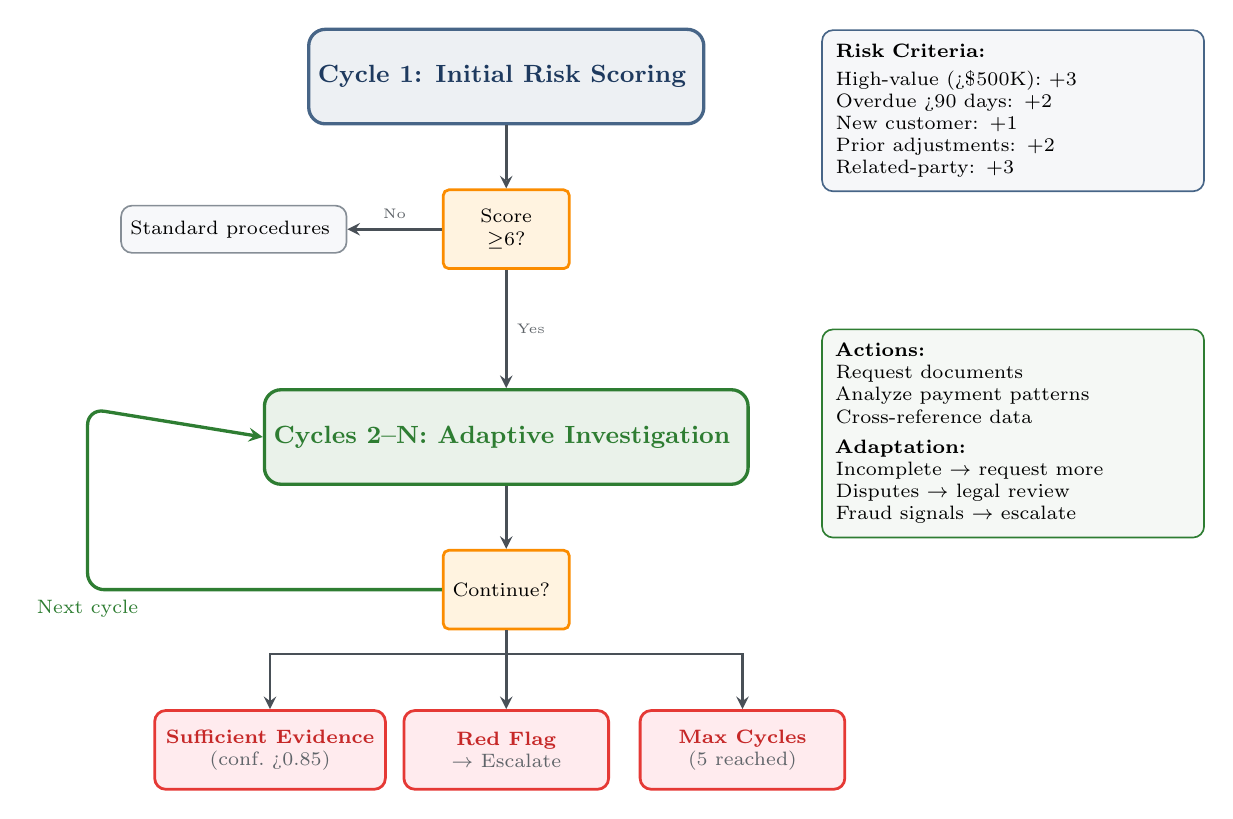
\begin{tikzpicture}[
    cycle box/.style={
        rounded corners=6pt,
        draw=#1,
        line width=1.2pt,
        fill=#1!10,
        minimum width=5cm,
        minimum height=1.2cm,
        font=\small,
        align=center
    },
    detail box/.style={
        rounded corners=4pt,
        draw=#1,
        line width=0.6pt,
        fill=#1!5,
        text width=4.5cm,
        inner sep=5pt,
        font=\scriptsize,
        align=left
    },
    decision/.style={
        rounded corners=2pt,
        draw=amber-600,
        line width=1pt,
        fill=amber-100,
        minimum width=1.6cm,
        minimum height=1cm,
        inner sep=3pt,
        font=\scriptsize,
        align=center
    },
    termination/.style={
        rounded corners=4pt,
        draw=red-600,
        line width=1pt,
        fill=red-100,
        minimum width=2.6cm,
        minimum height=1cm,
        inner sep=4pt,
        font=\scriptsize,
        align=center
    },
    lowrisk/.style={
        rounded corners=4pt,
        draw=gray-500,
        line width=0.6pt,
        fill=gray-100,
        minimum width=2.2cm,
        minimum height=0.6cm,
        font=\scriptsize,
        align=center
    },
    arrow/.style={->, thick, gray-700, >=stealth, line width=1pt},
    loop arrow/.style={->, thick, green-900, >=stealth, line width=1.2pt},
    label text/.style={font=\tiny, text=gray-600}
]

% === CYCLE 1 with detail box ===
\node[cycle box=slate-700] (cycle1) at (-2.5,0) {
    \textbf{\textcolor{slate-900}{Cycle 1: Initial Risk Scoring}}
};

\node[detail box=slate-700, anchor=north west] (c1details) at (1.5,0.6) {
    \textbf{Risk Criteria:}\\[2pt]
    High-value (>\$500K): +3\\
    Overdue >90 days: +2\\
    New customer: +1\\
    Prior adjustments: +2\\
    Related-party: +3
};

% === DECISION 1 ===
\node[decision, below=0.8cm of cycle1] (dec1) {
    Score\\$\geq$6?
};

% Low risk exit - to the left
\node[lowrisk, left=1.2cm of dec1] (lowrisk) {
    Standard procedures
};

% === CYCLE 2-N with detail box ===
\node[cycle box=green-900, below=1.5cm of dec1] (cycle2) {
    \textbf{\textcolor{green-900}{Cycles 2--N: Adaptive Investigation}}
};

\node[detail box=green-900, anchor=north west] (c2details) at (1.5,-3.2) {
    \textbf{Actions:}\\
    Request documents\\
    Analyze payment patterns\\
    Cross-reference data\\[3pt]
    \textbf{Adaptation:}\\
    Incomplete $\rightarrow$ request more\\
    Disputes $\rightarrow$ legal review\\
    Fraud signals $\rightarrow$ escalate
};

% === DECISION 2 ===
\node[decision, below=0.8cm of cycle2] (dec2) {
    Continue?
};

% === TERMINATION OUTCOMES ===
\node[termination, below=1cm of dec2, xshift=-3cm] (term1) {
    \textbf{\textcolor{red-900}{Sufficient Evidence}}\\
    \textcolor{gray-600}{(conf.\ >0.85)}
};

\node[termination, below=1cm of dec2] (term2) {
    \textbf{\textcolor{red-900}{Red Flag}}\\
    \textcolor{gray-600}{$\rightarrow$ Escalate}
};

\node[termination, below=1cm of dec2, xshift=3cm] (term3) {
    \textbf{\textcolor{red-900}{Max Cycles}}\\
    \textcolor{gray-600}{(5 reached)}
};

% === ARROWS ===
% Cycle 1 to Decision 1
\draw[arrow] (cycle1.south) -- (dec1.north);

% Decision 1: Yes to Cycle 2
\draw[arrow] (dec1.south) -- node[right, label text] {Yes} (cycle2.north);

% Decision 1: No to low risk (left)
\draw[arrow] (dec1.west) -- node[above, label text] {No} (lowrisk.east);

% Cycle 2 to Decision 2
\draw[arrow] (cycle2.south) -- (dec2.north);

% Decision 2 to terminations
\draw[arrow] (dec2.south) -- ++(0,-0.3) -| (term1.north);
\draw[arrow] (dec2.south) -- (term2.north);
\draw[arrow] (dec2.south) -- ++(0,-0.3) -| (term3.north);

% Loop back arrow - on left side, wide enough to clear the box
\draw[loop arrow, rounded corners=6pt] (dec2.west) -- ++(-4.5,0) node[below, font=\scriptsize, text=green-900] {Next cycle} -- ++(0,2.3) -- (cycle2.west);

\end{tikzpicture}
\caption{Iterative investigation workflow with explainable adaptation. Cycle~1 scores accounts using risk criteria; high-risk accounts (score $\geq$6) proceed to iterative investigation. Cycles~2--N gather evidence and adapt strategy based on findings. Investigation terminates when sufficient evidence is obtained, a red flag requires escalation, or maximum cycles are reached.}
\label{fig:agents3-iterative-investigation}
\end{figure}


\textbf{Explainability Validation}:
\begin{itemize}
\item \textbf{Faithfulness}: Verify explanations match actual investigation logic by reviewing audit logs (do logged perceptions and actions align with explanations?).
\item \textbf{Completeness}: Confirm all material risk indicators that triggered escalation appear in explanations.
\item \textbf{Usefulness}: Senior auditor reviews cycle-level explanations and confirms they support professional judgment (``Does the system's escalation rationale justify senior auditor involvement?'').
\end{itemize}

\textbf{Workpaper Documentation}: The audit workpaper includes:
\begin{itemize}
\item Initial risk scoring methodology (Cycle 1 criteria).
\item Cycle-by-cycle investigation narrative (what the system perceived, what actions it took, why it adapted).
\item Escalation rationale (why this account required human review).
\item Senior auditor's assessment: ``We deployed an agentic audit assistant to investigate 47 high-risk receivables. The system iteratively gathered evidence across 2-5 cycles per account, adapting its strategy based on discovered documentation quality and anomaly patterns. It escalated 8 accounts for senior review due to identified red flags (revenue recognition concerns, collectability doubts). We reviewed the system's investigation logs, assessed the escalated accounts, and obtained sufficient appropriate audit evidence to support our conclusions.''
\end{itemize}

This agentic design satisfies PCAOB's requirement that auditors understand their methodology while demonstrating how iteration and adaptation improve audit effectiveness. The system's ability to \emph{learn} during investigation (adapting strategy based on discovered evidence) and \emph{escalate appropriately} (terminating when human judgment is required) exemplifies agentic governance in practice.

\subsection{Human Oversight Workflows}
\label{sec:agents3-human-oversight}
\glsadd{human-in-the-loop}
\glsadd{human-on-the-loop}
\glsadd{human-in-command}

Section~\ref{sec:agents3-autonomy-calibration} defined three oversight modes. This section operationalizes them through workflows, notification mechanisms, intervention interfaces, and escalation procedures.

\paragraph{HITL (Human-in-the-Loop): Approval Workflows}
HITL systems require human pre-approval before executing high-consequence actions. Implementation requires:

\begin{itemize}
\item \textbf{Approval Queue}: System generates a recommendation and adds it to a queue visible to authorized reviewers.
\item \textbf{Notification}: Alert the reviewer (email, dashboard notification, SMS for time-sensitive actions).
\item \textbf{Review Interface}: Present the recommendation, supporting evidence, system confidence, and options (approve, reject, modify, request more information).
\item \textbf{Accountability}: Log who approved, when, and any modifications made.
\item \textbf{Automation Bias Mitigation}: To prevent rubber stamping, randomize the presentation order of recommendations, periodically inject known-incorrect recommendations as controls, and track approval/rejection rates per reviewer (flag reviewers with suspiciously high approval rates).
\end{itemize}

\paragraph{HOTL (Human-on-the-Loop): Monitoring and Intervention}
HOTL systems operate autonomously but humans monitor and can intervene. Implementation requires:

\begin{itemize}
\item \textbf{Monitoring Dashboard}: Real-time or near-real-time display of system activity (actions taken, error rates, escalation triggers, user feedback).
\item \textbf{Escalation Triggers}: Define conditions requiring human review (e.g., low-confidence decisions <0.7, user complaints, outcomes near policy boundaries, anomalies detected).
\item \textbf{Intervention Protocol}: How does the human halt the system, override a decision, or modify parameters? Must be accessible in real-time.
\item \textbf{Escalation Pathway}: If the monitoring human cannot resolve an issue, to whom do they escalate? (Senior supervisor, compliance officer, emergency stop authority.)
\end{itemize}

\textbf{Example: Agentic Credit Underwriting HOTL Monitoring.}
A mortgage lender's agentic underwriting system (described in Section~\ref{sec:agents3-audit-logging}) operates in HOTL mode, iteratively investigating applications across multiple cycles. Senior underwriters monitor aggregate system performance through a dashboard (\Cref{fig:agents3-hotl-dashboard}) displaying agentic-specific metrics and escalation triggers. When escalation frequency spikes or average cycles increase significantly, supervisors investigate root causes such as data quality degradation, overly conservative termination thresholds, or emerging risk patterns requiring strategy adjustment.

% HOTL Monitoring Dashboard - Agentic Credit Underwriting

\begin{figure}[htbp]
\centering
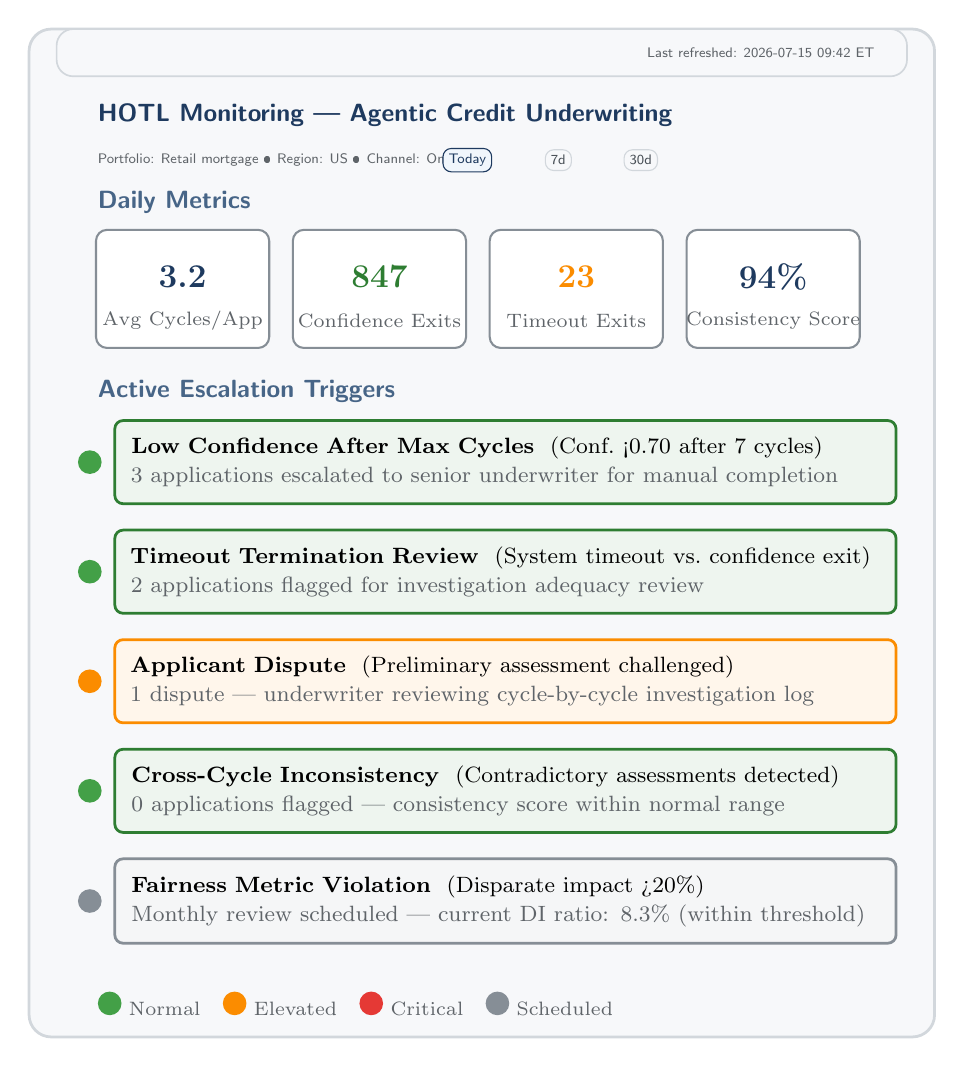
\begin{tikzpicture}[
    metric box/.style={
        rounded corners=4pt,
        draw=gray-500,
        line width=0.75pt,
        fill=white,
        minimum width=2.2cm,
        minimum height=1.5cm,
        font=\small,
        align=center
    },
    metric value/.style={font=\large\bfseries},
    metric label/.style={font=\scriptsize, text=gray-600},
    alert box/.style={
        rounded corners=3pt,
        draw=#1,
        line width=1pt,
        fill=#1!8,
        text width=9.5cm,
        inner sep=6pt,
        font=\footnotesize
    },
    section header/.style={
        font=\small\bfseries\sffamily,
        text=slate-700,
        anchor=west
    },
    status indicator/.style={
        circle,
        minimum size=0.3cm,
        inner sep=0pt
    },
    dashboard frame/.style={
        rounded corners=8pt,
        draw=gray-300,
        line width=1pt,
        fill=bg-neutral,
        inner sep=10pt
    },
    pill filter/.style={
        rounded corners=3pt,
        draw=gray-300,
        fill=gray-100,
        inner sep=2pt,
        font=\tiny\sffamily,
        text=gray-700
    },
    pill filter active/.style={
        pill filter,
        draw=primary,
        text=primary,
        fill=definition-light
    },
    meta label/.style={
        font=\tiny\sffamily,
        text=gray-600
    }
]

% Main dashboard frame
\node[dashboard frame, minimum width=11.5cm, minimum height=12.8cm] (frame) at (0,-4.6) {};

% Application chrome (top navigation bar)
\node[
    rounded corners=6pt,
    draw=gray-300,
    line width=0.6pt,
    fill=gray-100,
    minimum width=10.8cm,
    minimum height=0.6cm
] (topbar) at (0,1.5) {};
\node[meta label, anchor=east] at ([xshift=-0.3cm]topbar.east) {Last refreshed: 2026-07-15 09:42 ET};

% Dashboard view title and filters
\node[font=\small\bfseries\sffamily, text=slate-900, anchor=west] (viewtitle) at (-5.0,0.7) {HOTL Monitoring --- Agentic Credit Underwriting};
\node[meta label, anchor=west] at ([yshift=-0.3cm]viewtitle.south west) {Portfolio: Retail mortgage \textbullet\ Region: US \textbullet\ Channel: Online};
\node[pill filter active, anchor=west] at ([xshift=4.5cm,yshift=-0.3cm]viewtitle.south west) {Today};
\node[pill filter, anchor=west] at ([xshift=5.8cm,yshift=-0.3cm]viewtitle.south west) {7d};
\node[pill filter, anchor=west] at ([xshift=6.8cm,yshift=-0.3cm]viewtitle.south west) {30d};

% === METRICS ROW ===
\node[section header] at (-5.0,-0.4) {Daily Metrics};

% Metric 1: Avg Cycles
\node[metric box] (m1) at (-3.8,-1.5) {};
\node[metric value, text=slate-900] at ([yshift=0.15cm]m1.center) {3.2};
\node[metric label] at ([yshift=-0.4cm]m1.center) {Avg Cycles/App};

% Metric 2: Confidence Exits
\node[metric box] (m2) at (-1.3,-1.5) {};
\node[metric value, text=example-dark] at ([yshift=0.15cm]m2.center) {847};
\node[metric label] at ([yshift=-0.4cm]m2.center) {Confidence Exits};

% Metric 3: Timeout Exits
\node[metric box] (m3) at (1.2,-1.5) {};
\node[metric value, text=key-base] at ([yshift=0.15cm]m3.center) {23};
\node[metric label] at ([yshift=-0.4cm]m3.center) {Timeout Exits};

% Metric 4: Consistency Score
\node[metric box] (m4) at (3.7,-1.5) {};
\node[metric value, text=slate-900] at ([yshift=0.15cm]m4.center) {94\%};
\node[metric label] at ([yshift=-0.4cm]m4.center) {Consistency Score};

% === ESCALATION TRIGGERS ===
\node[section header] at (-5.0,-2.8) {Active Escalation Triggers};

% Alert 1 - Green (normal)
\node[alert box=example-dark] (a1) at (0.3,-3.7) {
    \textbf{Low Confidence After Max Cycles}~~\textnormal{(Conf.\ <0.70 after 7 cycles)}\\[1pt]
    \textcolor{gray-600}{3 applications escalated to senior underwriter for manual completion}
};
\node[status indicator, fill=example-base] at ([xshift=-0.3cm]a1.west) {};

% Alert 2 - Green (normal)
\node[alert box=example-dark, below=0.3cm of a1] (a2) {
    \textbf{Timeout Termination Review}~~\textnormal{(System timeout vs.\ confidence exit)}\\[1pt]
    \textcolor{gray-600}{2 applications flagged for investigation adequacy review}
};
\node[status indicator, fill=example-base] at ([xshift=-0.3cm]a2.west) {};

% Alert 3 - Amber (elevated)
\node[alert box=key-base, below=0.3cm of a2] (a3) {
    \textbf{Applicant Dispute}~~\textnormal{(Preliminary assessment challenged)}\\[1pt]
    \textcolor{gray-600}{1 dispute --- underwriter reviewing cycle-by-cycle investigation log}
};
\node[status indicator, fill=key-base] at ([xshift=-0.3cm]a3.west) {};

% Alert 4 - Green (normal)
\node[alert box=example-dark, below=0.3cm of a3] (a4) {
    \textbf{Cross-Cycle Inconsistency}~~\textnormal{(Contradictory assessments detected)}\\[1pt]
    \textcolor{gray-600}{0 applications flagged --- consistency score within normal range}
};
\node[status indicator, fill=example-base] at ([xshift=-0.3cm]a4.west) {};

% Alert 5 - Scheduled (gray)
\node[alert box=gray-500, below=0.3cm of a4] (a5) {
    \textbf{Fairness Metric Violation}~~\textnormal{(Disparate impact >20\%)}\\[1pt]
    \textcolor{gray-600}{Monthly review scheduled --- current DI ratio: 8.3\% (within threshold)}
};
\node[status indicator, fill=gray-500] at ([xshift=-0.3cm]a5.west) {};

% Legend
\node[font=\scriptsize, text=gray-600, anchor=north west] at (-5.0,-10.3) {
    \tikz\node[status indicator, fill=example-base] {}; Normal~~
    \tikz\node[status indicator, fill=key-base] {}; Elevated~~
    \tikz\node[status indicator, fill=caution-base] {}; Critical~~
    \tikz\node[status indicator, fill=gray-500] {}; Scheduled
};

\end{tikzpicture}
\caption{HOTL monitoring dashboard for agentic credit underwriting. The dashboard displays daily operational metrics (average investigation cycles, termination reasons, cross-cycle consistency) and active escalation triggers with status indicators. Senior underwriters monitor aggregate performance and intervene when triggers fire.}
\label{fig:agents3-hotl-dashboard}
\end{figure}


\paragraph{HIC (Human-in-Command): Strategic Oversight and Emergency Stop}
HIC systems operate with high autonomy. Humans set goals and constraints, monitor aggregate performance, and retain emergency stop authority. Implementation requires:

\begin{itemize}
\item \textbf{Strategic Goal-Setting}: Executives define objectives, risk appetite, and constraints (e.g., ``Fraud detection system must achieve 95\% precision, maintain false positive rate <1\%, and satisfy GDPR Article 22 requirements'').
\item \textbf{Aggregate Monitoring}: Statistical dashboards (daily/weekly/monthly) showing performance trends, fairness metrics, error rates, drift indicators. Not individual-decision review.
\item \textbf{Emergency Stop}: Accessible to authorized personnel (CTO, Chief Risk Officer, compliance head); tested quarterly; documented procedures for graceful shutdown (complete in-progress transactions, notify affected users, preserve state).
\item \textbf{Revalidation Triggers}: Define when the system must be revalidated before continuing operation (e.g., fairness violation detected, accuracy below SLA, regulatory policy change).
\end{itemize}

\subsection{Vendor Management}
\label{sec:agents3-vendor-management}

\glsadd{hallucination}Most organizations procure AI systems from vendors rather than building in-house. Vendor risk cascades into organizational liability: if the vendor's model hallucinates, is biased, or breaches confidentiality, the deploying organization faces regulatory penalties and reputational harm. Governance must include vendor due diligence, contract negotiation, and ongoing monitoring.

\paragraph{Vendor Due Diligence Framework (Three Phases)}
The framework proceeds through three phases. \textbf{Phase 1 (Assessment)} uses questionnaires to gather information about the vendor's data sources, model architecture, security practices, performance benchmarks, and fairness testing methodology. \textbf{Phase 2 (Document Review)} examines supporting documentation to verify vendor claims. This includes SOC 2 reports, data processing agreements, model validation reports, and security certifications. \textbf{Phase 3 (Validation)} confirms claims through reference checks with existing clients in similar domains and pilot testing with representative data to validate accuracy, explainability, and performance before full deployment.

% Three-Phase Vendor Due Diligence - Horizontal Flow

\begin{figure}[htbp]
\centering
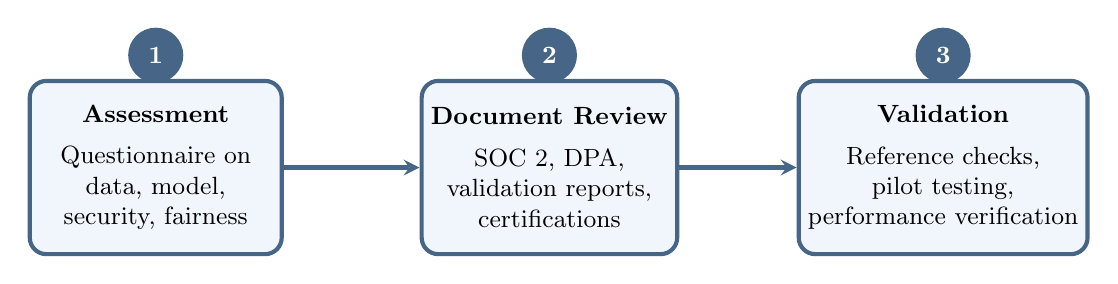
\begin{tikzpicture}[
    phase box/.style={
        rounded corners=6pt,
        draw=slate-700,
        line width=1.5pt,
        fill=slate-100,
        minimum width=3.2cm,
        minimum height=2.2cm,
        font=\small,
        align=center
    },
    phase number/.style={
        circle,
        fill=slate-700,
        text=white,
        font=\bfseries\small,
        minimum size=0.7cm,
        inner sep=0pt
    },
    arrow/.style={->, thick, slate-700, >=stealth, line width=1.5pt}
]

% Phase 1
\node[phase box] (phase1) at (0,0) {
    \textbf{Assessment}\\[4pt]
    Questionnaire on\\
    data, model,\\
    security, fairness
};
\node[phase number] at ([yshift=0.3cm]phase1.north) {1};

% Phase 2
\node[phase box] (phase2) at (5,0) {
    \textbf{Document Review}\\[4pt]
    SOC 2, DPA,\\
    validation reports,\\
    certifications
};
\node[phase number] at ([yshift=0.3cm]phase2.north) {2};

% Phase 3
\node[phase box] (phase3) at (10,0) {
    \textbf{Validation}\\[4pt]
    Reference checks,\\
    pilot testing,\\
    performance verification
};
\node[phase number] at ([yshift=0.3cm]phase3.north) {3};

% Arrows
\draw[arrow] (phase1.east) -- (phase2.west);
\draw[arrow] (phase2.east) -- (phase3.west);

\end{tikzpicture}
\caption{Three-phase vendor due diligence framework. Phase 1 gathers information through questionnaires; Phase 2 reviews supporting documentation and certifications; Phase 3 validates claims through reference checks and pilot testing with representative data.}
\label{fig:agents3-vendor-diligence}
\end{figure}


\paragraph{Contract Negotiation: Shifting Risk to Vendors Where Possible}
Negotiate contract terms that allocate risk appropriately:

\begin{table}[htbp]
\centering
\small
\begin{tabular}{>{\raggedright\arraybackslash}p{2.8cm} >{\raggedright\arraybackslash}p{7.8cm}}
\toprule
\textbf{Contract Term} & \textbf{Negotiation Focus} \\
\midrule
Liability Caps & Higher/uncapped liability for confidentiality breaches and negligence in high-risk cases \\
\addlinespace
Update Notification & 30-60 days advance notice before material model updates \\
\addlinespace
Audit Rights & Annual audits or upon incident discovery \\
\addlinespace
Data Handling & Prohibit training on customer data; deletion upon termination \\
\addlinespace
SLAs & Performance thresholds with specified remedies \\
\bottomrule
\end{tabular}
\caption{Key contract terms for allocating risk in AI vendor agreements.}
\label{tab:agents3-contract-terms}
\end{table}

\paragraph{Agentic-Specific Risk: Adaptation Opacity}
Agentic systems that learn and adapt create a unique vendor risk that traditional AI contracts do not address: \textbf{adaptation opacity}—the vendor's model silently updates its decision-making strategy in the background without formal version changes, invalidating continuous validation requirements and creating regulatory exposure.

\textbf{The Problem}: Regulatory frameworks like SR 11-7 (Federal Reserve model risk management) require ongoing validation of models used by banking institutions \parencite{fed-sr11-7}. Organizations validate ``Model v2.1'' and deploy it. If the vendor's agentic system \emph{adapts}—adjusting feature weights, refining decision criteria, or modifying iteration logic—the deployed system may behave materially differently from the validated version, yet the vendor does not issue a new version number or notify the customer. The organization continues operating under the assumption it is using validated ``v2.1,'' but the system's actual behavior has drifted. This breaks continuous validation, exposes the organization to regulatory penalties (``You deployed an unvalidated model''), and creates fairness risk (adaptation may introduce prohibited discrimination).

\textbf{Why Traditional Contracts Fail}: Standard AI vendor contracts address \emph{formal version updates} (``Vendor will notify Customer of material updates''). But agentic systems' adaptation mechanisms operate \emph{within} a version, not across versions. The vendor's position: ``We did not update the model—v2.1 is still v2.1. The system is designed to adapt; that is a feature, not a bug.'' The customer's regulatory obligation: ``We must validate material changes to model behavior, regardless of version numbering.''

\textbf{Contractual Mitigation—Adaptation Transparency Clauses}: For agentic vendor systems, negotiate contractual provisions that address adaptation opacity:

\begin{table}[htbp]
\centering
\small
\begin{tabular}{>{\raggedright\arraybackslash}p{3.2cm} >{\raggedright\arraybackslash}p{7.4cm}}
\toprule
\textbf{Clause Type} & \textbf{Purpose} \\
\midrule
Adaptation Disclosure & Vendor identifies all adaptation mechanisms; specifies static vs. adaptive components \\
\addlinespace
Change Log Access & API/dashboard access to logs showing changes, timing, and rationale \\
\addlinespace
Material Change Thresholds & Triggers requiring notification and revalidation rights \\
\addlinespace
Audit Rights & Periodic behavioral validation; vendor cooperation with audits \\
\addlinespace
Adaptation Freeze & Option to disable learning during exams or investigations \\
\bottomrule
\end{tabular}
\caption{Adaptation transparency clauses for agentic vendor contracts.}
\label{tab:agents3-adaptation-clauses}
\end{table}

\begin{tcolorbox}[
  enhanced,
  colback=bg-example,
  colframe=example-base,
  coltitle=white,
  fonttitle=\bfseries,
  title={Example Contractual Language: Adaptation Transparency},
  boxrule=1pt,
  left=3mm,
  right=3mm,
  top=2mm,
  bottom=2mm,
  breakable
]
\small
\textbf{Section X: Adaptation Transparency and Change Control}

\textbf{X.1 Adaptation Disclosure.} Vendor has disclosed in Exhibit C all mechanisms by which the System adapts its decision-making logic, including feature weight updates, threshold adjustments, and strategy refinements. Vendor represents that Exhibit C is complete and accurate as of the Effective Date.

\textbf{X.2 Change Logs.} Vendor shall maintain detailed change logs documenting all adaptation events, including timestamp, changed parameters, magnitude of change, and triggering feedback. Customer shall have API access to change logs with daily refresh.

\textbf{X.3 Material Change Notification.} If any of the following thresholds are met, Vendor shall notify Customer within five (5) business days and provide root cause analysis: (a) any feature weight changes by more than ten percent (10\%) absolute within thirty (30) days; (b) decision threshold changes by more than five percent (5\%) within thirty (30) days; (c) accuracy degrades by more than five percent (5\%) on validation dataset; or (d) disparate impact ratio for any protected class changes by more than ten percent (10\%).

\textbf{X.4 Revalidation Rights.} Upon Material Change notification, Customer may elect to: (a) require Vendor to revert System to last validated configuration (at no cost to Customer); (b) conduct revalidation testing (Vendor shall cooperate and bear reasonable costs); or (c) pause System operation pending resolution.

\textbf{X.5 Adaptation Freeze.} Upon forty-eight (48) hours' notice, Customer may require Vendor to disable all adaptation mechanisms, causing the System to operate with static parameters. Vendor shall maintain freeze mode for up to ninety (90) days per Calendar Year at no additional cost.
\end{tcolorbox}

\textbf{Governance Benefit}: These contractual provisions operationalize continuous validation requirements for adaptive agentic systems. Without adaptation transparency, organizations deploying vendor agentic systems face a compliance gap: regulatory obligations demand ongoing validation, but vendor opacity prevents detection of material changes. Adaptation transparency clauses shift this burden back to vendors and provide customers with the visibility necessary to satisfy SR 11-7, ECOA, and similar frameworks.

\paragraph{Ongoing Monitoring}
Vendor due diligence does not end at contract signature. Implement:
\begin{itemize}
\item \textbf{Performance Monitoring}: Track accuracy, error rates, user complaints. Compare vendor claims to observed performance.
\item \textbf{Security Monitoring}: Review vendor security incident reports; conduct annual security assessments.
\item \textbf{Accuracy Audits}: Quarterly or semi-annual testing of vendor outputs against ground truth.
\item \textbf{Escalation Procedures}: Define error rate thresholds triggering vendor review (e.g., ``If hallucination rate exceeds 5\%, escalate to General Counsel; consider vendor termination'').
\end{itemize}

\paragraph{Example: Law Firm Foundation Model Vetting}
A law firm evaluates a foundation model vendor for legal research assistance. Due diligence identifies five risk categories:

\begin{itemize}
\item \textbf{Confidentiality}: Vendor uses multi-tenant architecture; customer queries may be logged for training. \emph{Mitigation}: Negotiate zero-retention DPA; require vendor to delete all firm data within 30 days of session termination; annual audit rights.
\item \textbf{Conflicts}: Vendor serves competing law firms; could create conflicts if data is shared. \emph{Mitigation}: Vendor affirms data isolation per client; third-party audit confirms isolation controls.
\item \textbf{Accuracy}: Vendor claims 95\% citation accuracy but provides no independent validation. \emph{Mitigation}: Firm conducts pilot testing with 200 known cases; achieves 60\% accuracy (below acceptable threshold). Vendor contract includes accuracy SLA (90\%); quarterly accuracy audits; right to terminate if SLA violated for two consecutive quarters.
\item \textbf{Hallucination}: Model occasionally fabricates case law. \emph{Mitigation}: HITL verification (attorney must independently verify all citations before filing); firm maintains hallucination log; if hallucination rate >5\%, escalate to General Counsel.
\item \textbf{Regulatory Compliance}: ABA Rule 1.6 confidentiality obligations. \emph{Mitigation}: Vendor contract includes uncapped liability for confidentiality breaches; cyber insurance confirmation.
\end{itemize}

Firm approves vendor with conditions: HITL verification mandatory, quarterly accuracy audits, annual security review, zero-retention DPA. This risk-calibrated approach enables use while protecting against residual vendor risks.

\subsection{Performance Monitoring and Incident Response}
\label{sec:agents3-monitoring-incident}

Governance is not a one-time validation but a continuous cycle. Systems must be monitored for performance degradation, fairness violations, data drift, and security incidents. When failures occur, organizations must detect, contain, investigate, remediate, and learn. This shift from inspection-based to continuous monitoring mirrors the evolution of Statistical Process Control in manufacturing---a historical parallel we examined in Chapter~2.

% Incident Response Cycle - Vertical Flow with Full Descriptions
% Redesigned for US Trade 6x9 format (text width ~11.75cm)

\begin{figure}[htbp]
\centering
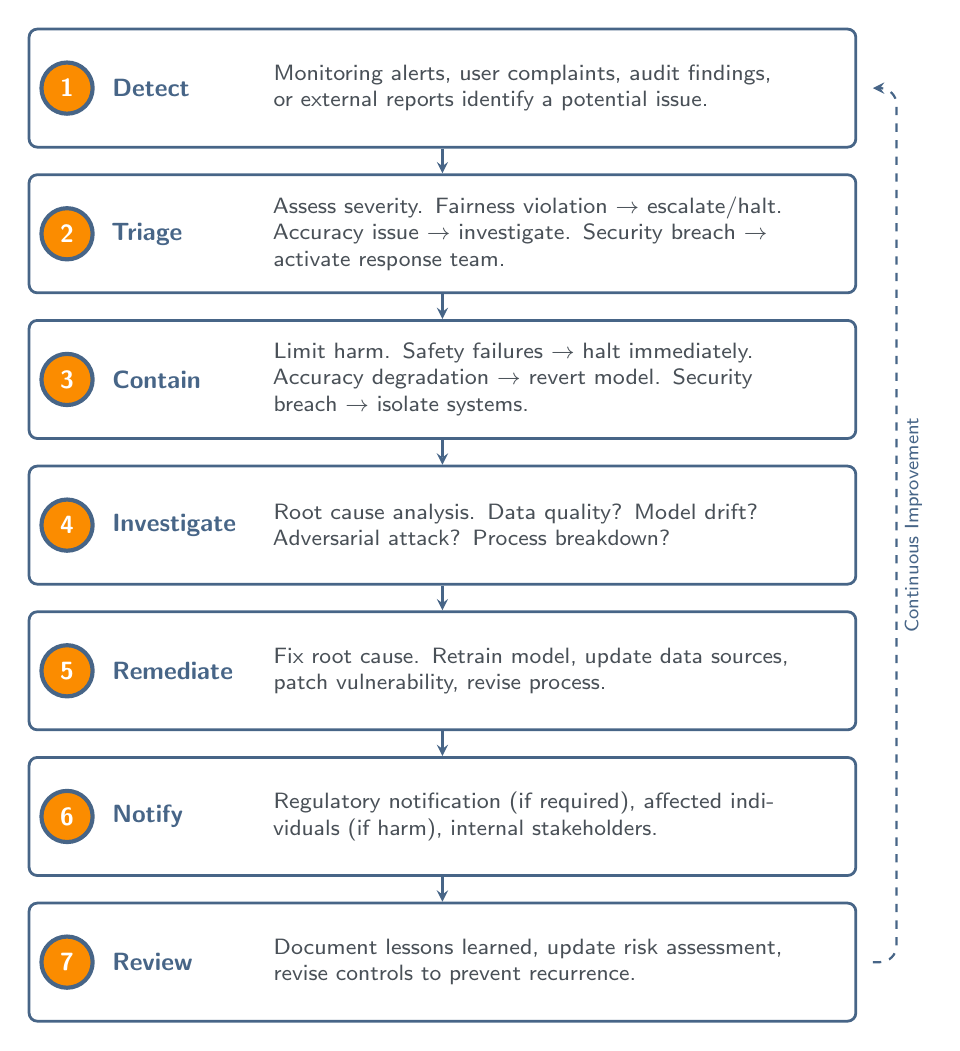
\begin{tikzpicture}[
    stage box/.style={
        draw=slate-700,
        line width=1pt,
        fill=white,
        rounded corners=3pt,
        minimum width=10.5cm,
        minimum height=1.5cm,
        inner sep=6pt
    },
    stage num/.style={
        circle,
        draw=slate-700,
        line width=1.5pt,
        fill=amber-600,
        text=white,
        font=\small\bfseries\sffamily,
        minimum size=0.65cm,
        inner sep=0pt
    },
    stage title/.style={
        font=\small\bfseries\sffamily,
        text=slate-700,
        anchor=west,
        text width=1.6cm
    },
    stage desc/.style={
        font=\footnotesize\sffamily,
        text=gray-700,
        text width=6.5cm,
        align=left
    },
    arrow/.style={->, thick, slate-700, >=stealth}
]

% Vertical spacing
\def\vstep{1.85cm}

% Stage 1 - Detect
\node[stage box] (s1) at (0, 0) {};
\node[stage num] at ([xshift=0.5cm]s1.west) {1};
\node[stage title] at ([xshift=0.95cm]s1.west) {Detect};
\node[stage desc, anchor=west] at ([xshift=3.0cm]s1.west) {Monitoring alerts, user complaints, audit findings, or external reports identify a potential issue.};

% Stage 2 - Triage
\node[stage box] (s2) at (0, -\vstep) {};
\node[stage num] at ([xshift=0.5cm]s2.west) {2};
\node[stage title] at ([xshift=0.95cm]s2.west) {Triage};
\node[stage desc, anchor=west] at ([xshift=3.0cm]s2.west) {Assess severity. Fairness violation $\rightarrow$ escalate/halt. Accuracy issue $\rightarrow$ investigate. Security breach $\rightarrow$ activate response team.};

% Stage 3 - Contain
\node[stage box] (s3) at (0, -2*\vstep) {};
\node[stage num] at ([xshift=0.5cm]s3.west) {3};
\node[stage title] at ([xshift=0.95cm]s3.west) {Contain};
\node[stage desc, anchor=west] at ([xshift=3.0cm]s3.west) {Limit harm. Safety failures $\rightarrow$ halt immediately. Accuracy degradation $\rightarrow$ revert model. Security breach $\rightarrow$ isolate systems.};

% Stage 4 - Investigate
\node[stage box] (s4) at (0, -3*\vstep) {};
\node[stage num] at ([xshift=0.5cm]s4.west) {4};
\node[stage title] at ([xshift=0.95cm]s4.west) {Investigate};
\node[stage desc, anchor=west] at ([xshift=3.0cm]s4.west) {Root cause analysis. Data quality? Model drift? Adversarial attack? Process breakdown?};

% Stage 5 - Remediate
\node[stage box] (s5) at (0, -4*\vstep) {};
\node[stage num] at ([xshift=0.5cm]s5.west) {5};
\node[stage title] at ([xshift=0.95cm]s5.west) {Remediate};
\node[stage desc, anchor=west] at ([xshift=3.0cm]s5.west) {Fix root cause. Retrain model, update data sources, patch vulnerability, revise process.};

% Stage 6 - Notify
\node[stage box] (s6) at (0, -5*\vstep) {};
\node[stage num] at ([xshift=0.5cm]s6.west) {6};
\node[stage title] at ([xshift=0.95cm]s6.west) {Notify};
\node[stage desc, anchor=west] at ([xshift=3.0cm]s6.west) {Regulatory notification (if required), affected individuals (if harm), internal stakeholders.};

% Stage 7 - Post-Incident Review
\node[stage box] (s7) at (0, -6*\vstep) {};
\node[stage num] at ([xshift=0.5cm]s7.west) {7};
\node[stage title] at ([xshift=0.95cm]s7.west) {Review};
\node[stage desc, anchor=west] at ([xshift=3.0cm]s7.west) {Document lessons learned, update risk assessment, revise controls to prevent recurrence.};

% Arrows between stages
\draw[arrow] (s1.south) -- (s2.north);
\draw[arrow] (s2.south) -- (s3.north);
\draw[arrow] (s3.south) -- (s4.north);
\draw[arrow] (s4.south) -- (s5.north);
\draw[arrow] (s5.south) -- (s6.north);
\draw[arrow] (s6.south) -- (s7.north);

% Feedback loop arrow from Review back to Detect
\draw[arrow, rounded corners=6pt, dashed]
    ([xshift=0.2cm]s7.east) -- ([xshift=0.5cm]s7.east) -- ([xshift=0.5cm]s1.east) -- ([xshift=0.2cm]s1.east);
\node[font=\scriptsize\sffamily, text=slate-700, rotate=90, anchor=south] at ([xshift=0.95cm, yshift=-5.55cm]s1.east) {Continuous Improvement};

\end{tikzpicture}
\caption{The seven-stage incident response cycle for AI system failures. The dashed feedback loop emphasizes that post-incident review improves detection capabilities, creating continuous improvement in governance controls.}
\label{fig:agents3-incident-response-cycle}
\end{figure}


\paragraph{Performance Monitoring: Four Dimensions}
Monitor continuously across four dimensions:

\begin{enumerate}
\item \textbf{Performance Metrics}: Accuracy, precision, recall, F1 score, latency—whatever aligns with business objectives. Establish SLAs and alert when performance degrades below thresholds.
\item \textbf{Data Drift}: Are input distributions changing? If the system was trained on 2020-2022 mortgage applications and is now seeing 2024 applications with different characteristics (higher interest rates, different applicant demographics), performance may degrade.
\item \textbf{Concept Drift}: Are input-output relationships changing? In practice, fraud patterns evolve; a fraud detection model trained on 2022 patterns may miss 2024 attack vectors.
\item \textbf{Fairness Metrics}: For systems affecting protected classes, monitor approval rates, error rates, and disparate impact ratios by demographic group. Regulatory expectations and enforcement practice under ECOA effectively require lenders to monitor for disparate impact as part of fair lending compliance. Similarly, GDPR Article 22 requires ongoing assessment of automated decision-making.
\end{enumerate}

\paragraph{Example: Disparate Impact in Agentic Credit Underwriting}
A regional bank deploys an agentic mortgage underwriting system that iteratively investigates applicants: it performs initial risk scoring, requests documentation based on risk indicators, adapts its investigation strategy based on applicant responses, and terminates when sufficient information is gathered or confidence thresholds trigger human escalation. \textit{Dimensional profile: HIC + institutional frame + adaptive goals + stateful.}

During routine monthly fairness monitoring, the compliance team detects a significant disparity: Hispanic applicants have a 65\% approval rate compared to 82\% for white applicants. This represents a clear violation of the 80\% rule commonly used in disparate impact analysis (65/82 = 79.3\%). Following the Tier 3 escalation pathway for critical issues (see \Cref{fig:agents3-escalation-example}), the compliance analyst immediately notifies the Chief Risk Officer, who halts the system and escalates to the CEO within hours of detection (\Cref{fig:agents3-incident-email-discovery}).

% Credit Underwriting Incident - Discovery Email from CRO to CEO

\begin{figure}[htbp]
\centering
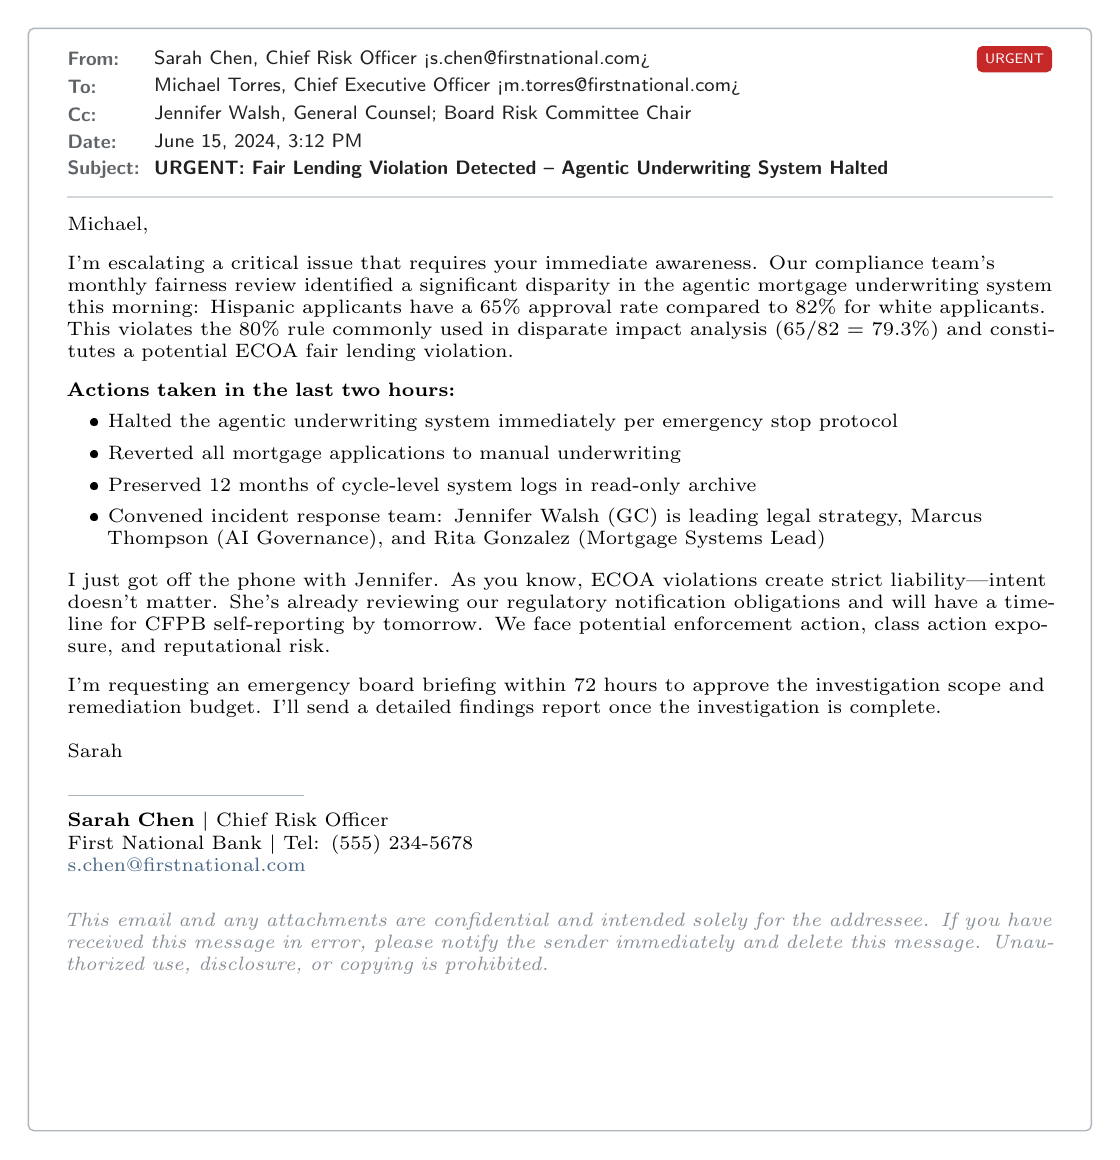
\begin{tikzpicture}[
    every node/.style={inner sep=0pt}
]

% Document frame
\node[
    draw=gray-400,
    line width=0.5pt,
    fill=white,
    minimum width=13.5cm,
    minimum height=14.0cm,
    rounded corners=2pt
] (page) at (0,0) {};

% Email header fields
\node[font=\scriptsize\sffamily, text=gray-600, anchor=west] at ([xshift=0.5cm, yshift=-0.4cm]page.north west) {\textbf{From:}};
\node[font=\scriptsize\sffamily, text=gray-900, anchor=west] at ([xshift=1.6cm, yshift=-0.4cm]page.north west) {Sarah Chen, Chief Risk Officer <s.chen@firstnational.com>};

\node[font=\scriptsize\sffamily, text=gray-600, anchor=west] at ([xshift=0.5cm, yshift=-0.75cm]page.north west) {\textbf{To:}};
\node[font=\scriptsize\sffamily, text=gray-900, anchor=west] at ([xshift=1.6cm, yshift=-0.75cm]page.north west) {Michael Torres, Chief Executive Officer <m.torres@firstnational.com>};

\node[font=\scriptsize\sffamily, text=gray-600, anchor=west] at ([xshift=0.5cm, yshift=-1.1cm]page.north west) {\textbf{Cc:}};
\node[font=\scriptsize\sffamily, text=gray-900, anchor=west] at ([xshift=1.6cm, yshift=-1.1cm]page.north west) {Jennifer Walsh, General Counsel; Board Risk Committee Chair};

\node[font=\scriptsize\sffamily, text=gray-600, anchor=west] at ([xshift=0.5cm, yshift=-1.45cm]page.north west) {\textbf{Date:}};
\node[font=\scriptsize\sffamily, text=gray-900, anchor=west] at ([xshift=1.6cm, yshift=-1.45cm]page.north west) {June 15, 2024, 3:12 PM};

\node[font=\scriptsize\sffamily, text=gray-600, anchor=west] at ([xshift=0.5cm, yshift=-1.8cm]page.north west) {\textbf{Subject:}};
\node[font=\scriptsize\bfseries\sffamily, text=gray-900, anchor=west] at ([xshift=1.6cm, yshift=-1.8cm]page.north west) {URGENT: Fair Lending Violation Detected -- Agentic Underwriting System Halted};

% Priority indicator
\node[font=\tiny\sffamily, text=white, fill=red-900, rounded corners=2pt, inner sep=3pt, anchor=east] at ([xshift=-0.5cm, yshift=-0.4cm]page.north east) {URGENT};

% Horizontal rule
\draw[gray-300, line width=0.5pt] ([xshift=0.5cm, yshift=-2.15cm]page.north west) -- ([xshift=-0.5cm, yshift=-2.15cm]page.north east);

% Email body
\node[
    text width=12.5cm,
    anchor=north west,
    font=\scriptsize,
    align=left
] at ([xshift=0.5cm, yshift=-2.4cm]page.north west) {
Michael,\\[6pt]
I'm escalating a critical issue that requires your immediate awareness. Our compliance team's monthly fairness review identified a significant disparity in the agentic mortgage underwriting system this morning: Hispanic applicants have a 65\% approval rate compared to 82\% for white applicants. This violates the 80\% rule commonly used in disparate impact analysis (65/82 = 79.3\%) and constitutes a potential ECOA fair lending violation.\\[6pt]
\textbf{Actions taken in the last two hours:}\\[3pt]
\begin{tabular}{@{\hspace{1em}\textbullet~}p{11.5cm}@{}}
Halted the agentic underwriting system immediately per emergency stop protocol\\[1pt]
Reverted all mortgage applications to manual underwriting\\[1pt]
Preserved 12 months of cycle-level system logs in read-only archive\\[1pt]
Convened incident response team: Jennifer Walsh (GC) is leading legal strategy, Marcus Thompson (AI Governance), and Rita Gonzalez (Mortgage Systems Lead)\\
\end{tabular}\\[6pt]
I just got off the phone with Jennifer. As you know, ECOA violations create strict liability---intent doesn't matter. She's already reviewing our regulatory notification obligations and will have a timeline for CFPB self-reporting by tomorrow. We face potential enforcement action, class action exposure, and reputational risk.\\[6pt]
I'm requesting an emergency board briefing within 72 hours to approve the investigation scope and remediation budget. I'll send a detailed findings report once the investigation is complete.\\[8pt]
Sarah\\[6pt]
\textcolor{gray-400}{\rule{3cm}{0.5pt}}\\[3pt]
\textbf{Sarah Chen}~\textbar~Chief Risk Officer\\
First National Bank~\textbar~Tel: (555) 234-5678\\
\textcolor{slate-700}{s.chen@firstnational.com}\\[12pt]
\textit{\textcolor{gray-500}{\scriptsize This email and any attachments are confidential and intended solely for the addressee. If you have received this message in error, please notify the sender immediately and delete this message. Unauthorized use, disclosure, or copying is prohibited.}}
};

\end{tikzpicture}
\caption{Initial escalation email from the Chief Risk Officer to CEO upon detection of a fair lending violation. The email documents immediate containment actions taken within two hours of detection, consistent with the Tier 3 escalation pathway for critical issues.}
\label{fig:agents3-incident-email-discovery}
\end{figure}


Ten weeks later, with the investigation complete and remediation implemented, the CRO sends a closure report (\Cref{fig:agents3-incident-email-closure}). The investigation reveals a governance challenge unique to agentic systems: the discrimination did not originate in the scoring model itself, which was facially neutral and passed traditional fairness testing. Instead, bias emerged through \emph{how the system investigated applicants across cycles}---Hispanic applicants triggered more verification cycles, leading to higher abandonment rates before final decisions were rendered. The system was discriminating in its \emph{process}, not its \emph{decisions}.

% Credit Underwriting Incident - Closure Email from CRO to CEO

\begin{figure}[htbp]
\centering

\begin{tikzpicture}[
    every node/.style={inner sep=0pt}
]

% Document frame
\node[
    draw=gray-400,
    line width=0.5pt,
    fill=white,
    minimum width=13.5cm,
    minimum height=20.2cm,
    rounded corners=2pt
] (page) at (0,0) {};

% Email header fields
\node[font=\scriptsize\sffamily, text=gray-600, anchor=west] at ([xshift=0.5cm, yshift=-0.4cm]page.north west) {\textbf{From:}};
\node[font=\scriptsize\sffamily, text=gray-900, anchor=west] at ([xshift=1.6cm, yshift=-0.4cm]page.north west) {Sarah Chen, Chief Risk Officer <s.chen@firstnational.com>};

\node[font=\scriptsize\sffamily, text=gray-600, anchor=west] at ([xshift=0.5cm, yshift=-0.75cm]page.north west) {\textbf{To:}};
\node[font=\scriptsize\sffamily, text=gray-900, anchor=west] at ([xshift=1.6cm, yshift=-0.75cm]page.north west) {Michael Torres, Chief Executive Officer <m.torres@firstnational.com>};

\node[font=\scriptsize\sffamily, text=gray-600, anchor=west] at ([xshift=0.5cm, yshift=-1.1cm]page.north west) {\textbf{Cc:}};
\node[font=\scriptsize\sffamily, text=gray-900, anchor=west] at ([xshift=1.6cm, yshift=-1.1cm]page.north west) {Jennifer Walsh, General Counsel; Board Risk Committee Chair};

\node[font=\scriptsize\sffamily, text=gray-600, anchor=west] at ([xshift=0.5cm, yshift=-1.45cm]page.north west) {\textbf{Date:}};
\node[font=\scriptsize\sffamily, text=gray-900, anchor=west] at ([xshift=1.6cm, yshift=-1.45cm]page.north west) {August 30, 2024, 4:47 PM};

\node[font=\scriptsize\sffamily, text=gray-600, anchor=west] at ([xshift=0.5cm, yshift=-1.8cm]page.north west) {\textbf{Subject:}};
\node[font=\scriptsize\bfseries\sffamily, text=gray-900, anchor=west, text width=10cm] at ([xshift=1.6cm, yshift=-1.8cm]page.north west) {CLOSED: Fair Lending Incident FL-2024-003 -- Findings and Remediation};

% Horizontal rule
\draw[gray-300, line width=0.5pt] ([xshift=0.5cm, yshift=-2.15cm]page.north west) -- ([xshift=-0.5cm, yshift=-2.15cm]page.north east);

% Email body
\node[
    text width=12.5cm,
    anchor=north west,
    font=\scriptsize,
    align=left
] at ([xshift=0.5cm, yshift=-2.4cm]page.north west) {
Michael,\\[6pt]
I'm pleased to confirm that Incident FL-2024-003 is now closed. The system has been remediated and redeployed. Here's what we found and what we've changed.\\[6pt]
\textbf{Root Cause: Process-Based Discrimination.} The discrimination wasn't in the scoring model---Cycle 1 risk assessment was facially neutral and passed our traditional fairness tests. The problem was \textit{how the system investigated applicants across subsequent cycles}:\\[3pt]
\begin{tabular}{@{\hspace{1em}\textbullet~}p{11.5cm}@{}}
Hispanic applicants triggered more verification cycles (5.2 avg vs. 3.8 for white applicants)\\[1pt]
The system had learned to flag shorter U.S. employment tenure for extra scrutiny---a proxy for national origin\\[1pt]
Extended verification led to higher abandonment: 28\% of Hispanic applicants withdrew vs. 12\% of white applicants\\
\end{tabular}\\[3pt]
The system wasn't discriminating in its \textit{decisions}---it was discriminating in its \textit{process}. Applicants who would have been approved were dropping out because we were investigating them more aggressively.\\[6pt]
\textbf{Remediation Implemented.} Rita Gonzalez and Marcus Thompson led the technical remediation. Before redeploying, we made four changes: (1) prohibited employment tenure from influencing investigation depth; (2) added cycle-count parity monitoring that flags deviations >20\% from demographic medians; (3) implemented abandonment tracking by protected class; and (4) retrained and revalidated the system for both outcome \textit{and} process fairness.\\[6pt]
\textbf{Regulatory and Applicant Notification.} Jennifer filed our self-report with the CFPB on July 12th, within the 30-day window the board approved. Her team has also sent notification letters to all 847 affected Hispanic applicants from the past 12 months, offering expedited re-review with human oversight, waived fees, and priority processing. So far, 312 have requested re-review.\\[6pt]
\textbf{What We're Changing Going Forward.} This one caught us off guard. Our fairness testing was focused on approval rates---we weren't looking at how the system \textit{investigated} people differently. I talked with Marcus yesterday, and he's already updating our AI Governance framework to treat ``iteration bias'' as a distinct risk category. We're revising our validation protocols to require fairness testing across the full investigation process, not just final decisions. We're also adding this to the quarterly model risk review.\\[6pt]
I'll present the full post-incident review at next month's board meeting, including proposed policy updates for all agentic systems.\\[8pt]
Sarah\\[6pt]
\textcolor{gray-400}{\rule{3cm}{0.5pt}}\\[3pt]
\textbf{Sarah Chen}~\textbar~Chief Risk Officer\\
First National Bank~\textbar~Tel: (555) 234-5678\\
\textcolor{slate-700}{s.chen@firstnational.com}\\[12pt]
\textit{\textcolor{gray-500}{\scriptsize This email and any attachments are confidential and intended solely for the addressee. If you have received this message in error, please notify the sender immediately and delete this message. Unauthorized use, disclosure, or copying is prohibited.}}
};

\end{tikzpicture}
\caption{Closure email summarizing investigation findings and remediation actions. The root cause---process-based discrimination through unequal verification burdens---represents a failure mode unique to agentic systems that traditional outcome-focused fairness testing would not detect.}
\label{fig:agents3-incident-email-closure}
\end{figure}


\textbf{Governance Principles Illustrated}:
\begin{itemize}
\item \textbf{Agentic fairness risk}: Discrimination emerges through \emph{how} the system iterates (process), not just final outcomes.
\item \textbf{Cross-cycle accountability}: Traditional fairness testing (outcome parity) is insufficient; organizations must audit investigation process across cycles.
\item \textbf{Adaptation constraints}: System learning must be constrained to prevent adaptation from introducing prohibited proxies.
\item \textbf{Termination parity}: Cycle-count monitoring ensures investigation burdens are distributed fairly across demographic groups.
\end{itemize}

These technical and operational controls require clear organizational ownership and accountability structures---the subject we turn to next.



% Section 5: Accountability and Organizational Structure
% ============================================================================
% Accountability and Organizational Structure — Agents Part III
% Purpose: Define roles, organizational models, and liability allocation
% Label: sec:agents3-accountability
% ============================================================================

\section{Accountability and Organizational Structure}
\label{sec:agents3-accountability}

Technical controls alone do not create accountability. Governance requires explicit assignment of roles and responsibilities: who approves deployments, who monitors performance, who investigates incidents, who escalates to regulators? This section presents three organizational governance models, demonstrates role assignment through RACI matrices, defines escalation and reporting structures, and examines liability allocation. The goal is to ensure every governance activity has a clearly accountable owner.

\subsection{Three Organizational Governance Models}
\label{sec:agents3-governance-models}

Organizations structure AI governance in three primary ways, each with advantages and disadvantages depending on size, AI maturity, and regulatory intensity.

\paragraph{Centralized Model: Single AI Governance Office}
A dedicated AI governance office or committee reports to senior leadership (typically the Chief Risk Officer, Chief Compliance Officer, or Chief Technology Officer). This office establishes policies, reviews all proposed AI deployments, conducts risk assessments, and monitors compliance. This model suits small to medium organizations (500-2,000 employees) with limited AI systems (5-20 use cases), high regulatory stakes (financial services, healthcare, legal), or early AI maturity where governance capability is being built.

\smallskip
\noindent
\begin{minipage}[t]{0.48\textwidth}
\vspace{0pt}
\begin{tcolorbox}[
  enhanced,
  colback=bg-example,
  colframe=example-dark,
  fonttitle=\bfseries,
  coltitle=white,
  title=Advantages,
  boxrule=1pt,
  arc=2pt,
  left=6pt, right=6pt, top=4pt, bottom=4pt,
  equal height group=centralized,
  valign=top
]
\small
\textbf{Consistency}: Single office ensures uniform governance standards across all systems.\\[3pt]
\textbf{Expertise concentration}: Governance specialists develop deep knowledge of regulatory requirements and best practices.\\[3pt]
\textbf{Clear accountability}: One office owns all AI governance decisions.\\[3pt]
\textbf{Easier audit}: Regulators and internal auditors interact with a single governance function.
\end{tcolorbox}
\end{minipage}%
\hfill
\begin{minipage}[t]{0.48\textwidth}
\vspace{0pt}
\begin{tcolorbox}[
  enhanced,
  colback=bg-caution,
  colframe=caution-dark,
  fonttitle=\bfseries,
  coltitle=white,
  title=Disadvantages,
  boxrule=1pt,
  arc=2pt,
  left=6pt, right=6pt, top=4pt, bottom=4pt,
  equal height group=centralized,
  valign=top
]
\small
\textbf{Bottleneck risk}: All deployment decisions route through one office, creating delays.\\[3pt]
\textbf{Limited domain expertise}: Central office may lack deep knowledge of domain-specific requirements (e.g., PCAOB audit standards, ECOA fair lending nuances).\\[3pt]
\textbf{Scalability}: As AI adoption grows, central office becomes overwhelmed.
\end{tcolorbox}
\end{minipage}

\medskip

\textbf{Example}: Regional investment advisory firm (500 employees, 10 AI tools) establishes AI Governance Office under Chief Compliance Officer with governance lead, technical specialist, and support staff conducting quarterly system reviews.

\paragraph{Federated Model: Central Coordination with Distributed Expertise}
A central AI governance function establishes enterprise-wide policies and standards, while domain-specific governance teams (e.g., audit practice AI lead, tax practice AI lead, wealth management AI lead) implement and monitor compliance within their areas. The central function coordinates, audits federated teams, and escalates enterprise-wide issues. This model suits large organizations (5,000+ employees) with diverse AI use cases across multiple domains (50+ systems), mature AI adoption, and domain-specific regulatory requirements (audit, legal, banking, securities).

\smallskip
\noindent
\begin{minipage}[t]{0.48\textwidth}
\vspace{0pt}
\begin{tcolorbox}[
  enhanced,
  colback=bg-example,
  colframe=example-dark,
  fonttitle=\bfseries,
  coltitle=white,
  title=Advantages,
  boxrule=1pt,
  arc=2pt,
  left=6pt, right=6pt, top=4pt, bottom=4pt,
  equal height group=federated,
  valign=top
]
\small
\textbf{Domain expertise}: Practice leads understand PCAOB standards, tax regulations, or wealth management suitability rules better than a central office.\\[3pt]
\textbf{Scalability}: Distributed teams prevent central bottlenecks.\\[3pt]
\textbf{Tailored governance}: Each domain calibrates controls to specific regulatory and risk contexts.
\end{tcolorbox}
\end{minipage}%
\hfill
\begin{minipage}[t]{0.48\textwidth}
\vspace{0pt}
\begin{tcolorbox}[
  enhanced,
  colback=bg-caution,
  colframe=caution-dark,
  fonttitle=\bfseries,
  coltitle=white,
  title=Disadvantages,
  boxrule=1pt,
  arc=2pt,
  left=6pt, right=6pt, top=4pt, bottom=4pt,
  equal height group=federated,
  valign=top
]
\small
\textbf{Inconsistency risk}: Different domains may interpret policies differently or adopt varying standards.\\[3pt]
\textbf{Coordination overhead}: Central function must monitor multiple federated teams.\\[3pt]
\textbf{Accountability diffusion}: Harder to pinpoint responsibility when governance is distributed.
\end{tcolorbox}
\end{minipage}

\medskip

\textbf{Example}: Big Four accounting firm (10,000 employees, 50+ AI tools) establishes central AI Governance Committee setting firm-wide policies while each practice (audit, tax, advisory) designates domain-specific AI Leads ensuring compliance with practice-specific regulations (PCAOB, IRS, client confidentiality).

\paragraph{Embedded Model: Governance Within Existing Functions}
AI governance is integrated into existing risk management, compliance, IT governance, and legal functions rather than creating a separate AI-specific structure. Each function applies its existing governance processes to AI systems. This model suits organizations with mature, well-functioning governance (strong ERM, compliance, IT governance), AI systems that extend existing processes (e.g., AI-enhanced fraud detection within existing fraud team), and leadership that prefers integration over new silos.

\smallskip
\noindent
\begin{minipage}[t]{0.48\textwidth}
\vspace{0pt}
\begin{tcolorbox}[
  enhanced,
  colback=bg-example,
  colframe=example-dark,
  fonttitle=\bfseries,
  coltitle=white,
  title=Advantages,
  boxrule=1pt,
  arc=2pt,
  left=6pt, right=6pt, top=4pt, bottom=4pt,
  equal height group=embedded,
  valign=top
]
\small
\textbf{Efficiency}: Leverages existing governance infrastructure.\\[3pt]
\textbf{Avoids silos}: Prevents AI governance from operating in isolation from enterprise risk management.\\[3pt]
\textbf{Cultural fit}: Organizations resistant to new bureaucracy prefer extending existing processes.
\end{tcolorbox}
\end{minipage}%
\hfill
\begin{minipage}[t]{0.48\textwidth}
\vspace{0pt}
\begin{tcolorbox}[
  enhanced,
  colback=bg-caution,
  colframe=caution-dark,
  fonttitle=\bfseries,
  coltitle=white,
  title=Disadvantages,
  boxrule=1pt,
  arc=2pt,
  left=6pt, right=6pt, top=4pt, bottom=4pt,
  equal height group=embedded,
  valign=top
]
\small
\textbf{Expertise gaps}: Existing functions may lack AI-specific knowledge (fairness testing, model validation, adversarial robustness).\\[3pt]
\textbf{Accountability ambiguity}: If AI governance is ``everyone's responsibility,'' it may become no one's priority.\\[3pt]
\textbf{Inconsistent application}: Different functions may apply AI governance unevenly.
\end{tcolorbox}
\end{minipage}

\medskip

This model requires AI-specific training for existing governance personnel and clear assignment of AI oversight responsibilities within each function.

\subsection{RACI Matrix: Operationalizing Accountability}
\label{sec:agents3-raci}

Regardless of governance model, organizations must assign accountability for each governance activity using a RACI framework:

\smallskip
\noindent
\begin{minipage}[t]{0.235\textwidth}
\vspace{0pt}
\begin{tcolorbox}[
  enhanced,
  colback=bg-definition,
  colframe=definition-base,
  fonttitle=\bfseries\Large,
  coltitle=white,
  title=\centering R,
  boxrule=1pt,
  arc=2pt,
  left=4pt, right=4pt, top=4pt, bottom=4pt,
  equal height group=raci,
  valign=top
]
\centering
\small\textbf{Responsible}\\[4pt]
\scriptsize Who does the work?\\[6pt]
\textit{May be multiple people}
\end{tcolorbox}
\end{minipage}%
\hfill
\begin{minipage}[t]{0.235\textwidth}
\vspace{0pt}
\begin{tcolorbox}[
  enhanced,
  colback=bg-definition,
  colframe=definition-base,
  fonttitle=\bfseries\Large,
  coltitle=white,
  title=\centering A,
  boxrule=1pt,
  arc=2pt,
  left=4pt, right=4pt, top=4pt, bottom=4pt,
  equal height group=raci,
  valign=top
]
\centering
\small\textbf{Accountable}\\[4pt]
\scriptsize Who has decision authority and ultimate accountability?\\[6pt]
\textit{\textbf{Only one A per activity}}
\end{tcolorbox}
\end{minipage}%
\hfill
\begin{minipage}[t]{0.235\textwidth}
\vspace{0pt}
\begin{tcolorbox}[
  enhanced,
  colback=bg-definition,
  colframe=definition-base,
  fonttitle=\bfseries\Large,
  coltitle=white,
  title=\centering C,
  boxrule=1pt,
  arc=2pt,
  left=4pt, right=4pt, top=4pt, bottom=4pt,
  equal height group=raci,
  valign=top
]
\centering
\small\textbf{Consulted}\\[4pt]
\scriptsize Who provides input or expertise before decisions?\\[6pt]
\textit{Two-way communication}
\end{tcolorbox}
\end{minipage}%
\hfill
\begin{minipage}[t]{0.235\textwidth}
\vspace{0pt}
\begin{tcolorbox}[
  enhanced,
  colback=bg-definition,
  colframe=definition-base,
  fonttitle=\bfseries\Large,
  coltitle=white,
  title=\centering I,
  boxrule=1pt,
  arc=2pt,
  left=4pt, right=4pt, top=4pt, bottom=4pt,
  equal height group=raci,
  valign=top
]
\centering
\small\textbf{Informed}\\[4pt]
\scriptsize Who is notified after decisions?\\[6pt]
\textit{One-way communication}
\end{tcolorbox}
\end{minipage}

\medskip
\noindent The key principle: \textbf{every governance activity must have exactly one Accountable party}. Diffused accountability (``the team is accountable'') creates gaps where no one takes ownership.

Table~\ref{tab:agents3-raci} provides a sample RACI matrix for AI governance activities.

\begin{table}[!ht]
\centering
\caption{Sample RACI Matrix for AI Governance Activities}
\label{tab:agents3-raci}
\footnotesize
\begin{tabular}{>{\raggedright\arraybackslash}p{4.0cm} >{\centering\arraybackslash}p{1.5cm} >{\centering\arraybackslash}p{1.4cm} >{\centering\arraybackslash}p{1.5cm} >{\centering\arraybackslash}p{1.5cm} >{\centering\arraybackslash}p{2.0cm}}
\toprule
\textbf{Activity} & \textbf{Board / CEO} & \textbf{CRO / CCO} & \textbf{AI Gov. Lead} & \textbf{System Owner} & \textbf{Legal / Compliance} \\
\midrule
Approve enterprise AI governance policy & A & C & R & I & C \\
\addlinespace
Approve low-risk AI deployment & I & I & A & R & C \\
\addlinespace
Approve high-risk AI deployment & A & C & R & R & C \\
\addlinespace
Conduct pre-deployment risk assessment & I & C & A & R & C \\
\addlinespace
Monitor system performance (ongoing) & I & I & C & A, R & I \\
\addlinespace
Investigate fairness violation & I & A & C & R & C \\
\addlinespace
Approve vendor contract (high-risk system) & I & A & C & R & C \\
\addlinespace
Report to board (quarterly AI governance update) & I & A & R & I & C \\
\addlinespace
Respond to regulatory inquiry & C & A & R & R & R \\
\bottomrule
\end{tabular}
\end{table}

\paragraph{Key Observations from the Matrix}:

\begin{itemize}
\item \textbf{Single Accountability}: Each activity has one A. For example, the CRO (Chief Risk Officer) is accountable for fairness violation investigations; the AI Governance Lead is accountable for low-risk deployments.

\item \textbf{Escalation}: High-risk deployments elevate accountability to the Board/CEO, while low-risk deployments can be approved by the AI Governance Lead. This prevents bottlenecks (Board does not review every chatbot deployment) while ensuring senior oversight for consequential systems.

\item \textbf{Multiple Responsible Parties}: Risk assessments may involve both the AI Governance Lead (methodological expertise) and the System Owner (domain knowledge). Both contribute, but only one is Accountable for the final approval.

\item \textbf{Consultation and Information Flow}: Legal and Compliance are Consulted on most activities, ensuring regulatory considerations inform decisions. The Board is Informed of governance activities but not burdened with operational details.
\end{itemize}

Organizations should customize this matrix to their structure, size, and regulatory context. The principle—single accountability per activity—remains universal.

\subsection{Escalation and Reporting}
\label{sec:agents3-escalation-reporting}

Governance requires clear escalation triggers: when must an operational issue be escalated to management, executives, or the board? And what cadence and format should governance reporting follow?

\paragraph{Three-Tier Escalation Model}

% Three-Tier Escalation Model - Traffic Light Visualization

\begin{figure}[htbp]
\centering
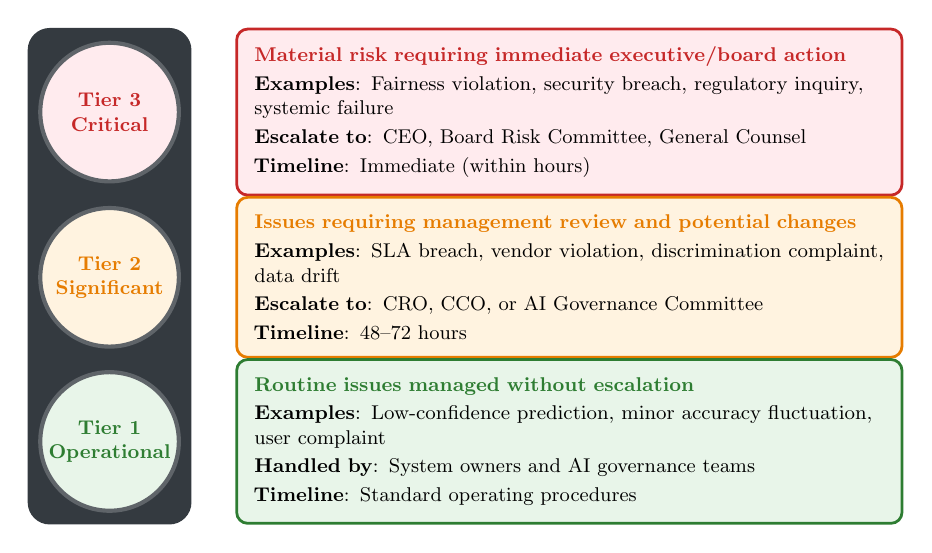
\begin{tikzpicture}[scale=0.80, every node/.append style={transform shape},
    remember picture,
    tier circle/.style={circle, minimum size=2.2cm, inner sep=0pt, draw=gray-600, line width=1.5pt, font=\bfseries\small, align=center},
    tier box/.style={rounded corners=4pt, draw=#1, line width=1pt, inner sep=8pt, text width=10cm, font=\small}
]

% Draw text boxes first to establish positions
% Tier 3 description box
\node[tier box=caution-dark, fill=bg-caution, anchor=north west] (box3) at (2.0,0) {%
\textbf{\textcolor{caution-dark}{Material risk requiring immediate executive/board action}}\\[2pt]
\textbf{Examples}: Fairness violation, security breach, regulatory inquiry, systemic failure\\[2pt]
\textbf{Escalate to}: CEO, Board Risk Committee, General Counsel\\[2pt]
\textbf{Timeline}: Immediate (within hours)
};

% Tier 2 description box - positioned directly below box3
\node[tier box=key-dark, fill=bg-key, anchor=north west] (box2) at (box3.south west) {%
\textbf{\textcolor{key-dark}{Issues requiring management review and potential changes}}\\[2pt]
\textbf{Examples}: SLA breach, vendor violation, discrimination complaint, data drift\\[2pt]
\textbf{Escalate to}: CRO, CCO, or AI Governance Committee\\[2pt]
\textbf{Timeline}: 48--72 hours
};

% Tier 1 description box - positioned directly below box2
\node[tier box=example-dark, fill=bg-example, anchor=north west] (box1) at (box2.south west) {%
\textbf{\textcolor{example-dark}{Routine issues managed without escalation}}\\[2pt]
\textbf{Examples}: Low-confidence prediction, minor accuracy fluctuation, user complaint\\[2pt]
\textbf{Handled by}: System owners and AI governance teams\\[2pt]
\textbf{Timeline}: Standard operating procedures
};

% Traffic light housing - fixed width centered at x=0
\fill[gray-800, rounded corners=8pt]
    (-1.3,0 |- box3.north) rectangle (1.3,0 |- box1.south);

% Calculate positions for circles using the center of each box
\node[tier circle, fill=bg-caution, text=caution-dark] (tier3) at (0,0 |- box3.center) {Tier 3\\Critical};
\node[tier circle, fill=bg-key, text=key-dark] (tier2) at (0,0 |- box2.center) {Tier 2\\Significant};
\node[tier circle, fill=bg-example, text=example-dark] (tier1) at (0,0 |- box1.center) {Tier 1\\Operational};

\end{tikzpicture}
\caption{Three-tier escalation model for AI governance issues. Tier 1 (operational) issues are handled routinely; Tier 2 (significant) issues require management review; Tier 3 (critical) issues demand immediate executive or board action. Pre-defining which issues fall into each tier ensures rapid, consistent response.}
\label{fig:agents3-escalation-tiers}
\end{figure}


\paragraph{Reporting Cadence and Audience}

\textbf{Operational Dashboards (Daily/Weekly)}: System owners and AI governance teams monitor real-time or near-real-time dashboards showing performance metrics, error rates, escalation counts, user feedback. These are working tools, not executive reports.

\textbf{Management Reports (Monthly/Quarterly)}: Chief Risk Officer and Chief Compliance Officer receive summary reports: number of systems deployed, risk assessments completed, incidents investigated, SLA compliance, vendor performance, upcoming regulatory developments. Format: 2-5 page executive summary with supporting appendices.

\textbf{Board Presentations (Quarterly/Annual)}: Board receives narrative synthesis: strategic governance posture (are we ahead of or behind regulatory curve?), high-risk system approvals, material incidents and responses, policy changes, budget and resource requests. Format: 10-15 slide deck; focus on risk appetite alignment, not operational details.

\paragraph{Example Escalation: Fairness Violation in Credit Decisioning}
A bank's monthly fairness monitoring detects disparate impact in credit pre-screening (see Section~\ref{sec:agents3-monitoring-incident}). Figure~\ref{fig:agents3-escalation-example} illustrates the Tier 1 → Tier 3 escalation pathway, demonstrating how pre-defined critical issues trigger rapid organizational response with specific time targets at each stage.

% Example Escalation: Fairness Violation - Vertical Timeline

\begin{figure}[htbp]
\centering
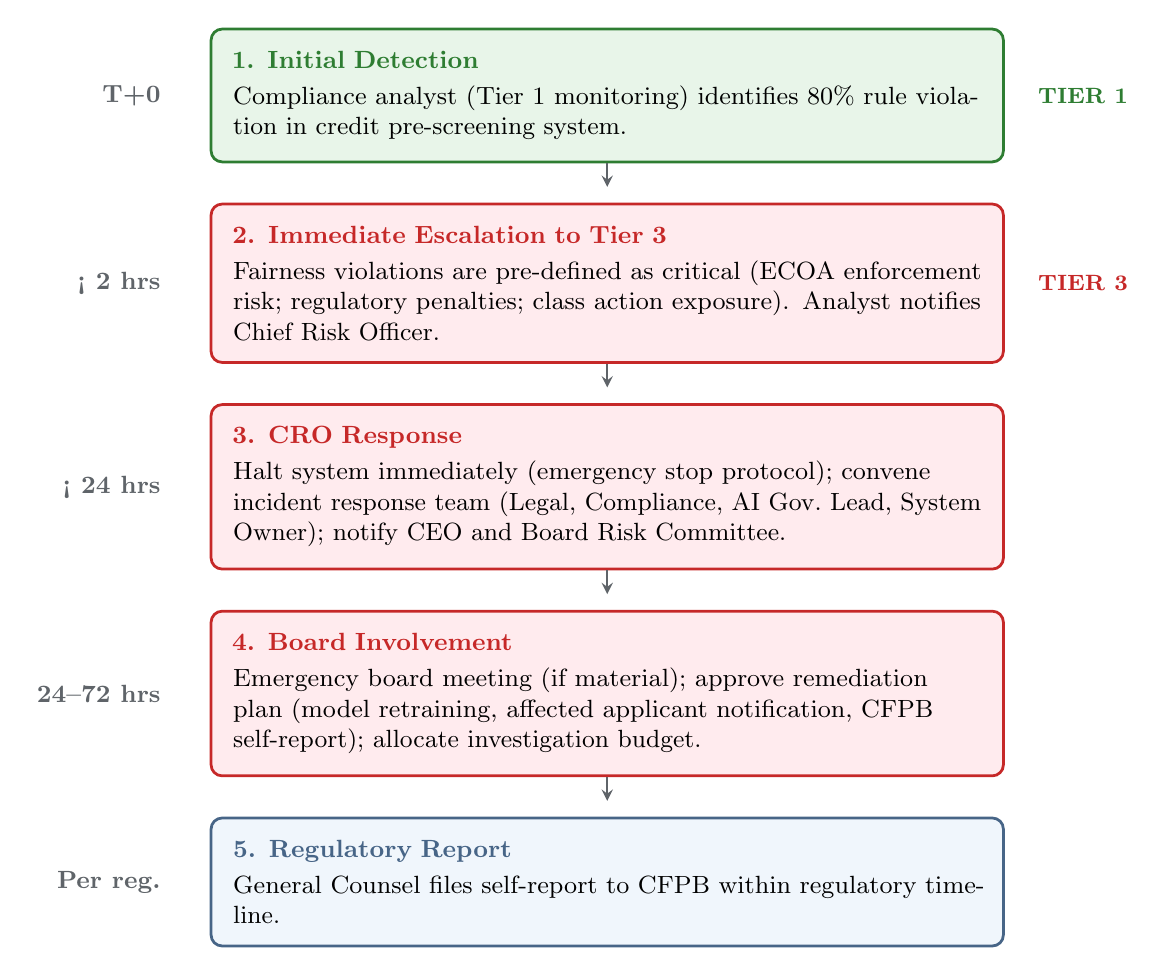
\begin{tikzpicture}[
    step box/.style={rounded corners=4pt, draw=#1, line width=1pt, inner sep=8pt, text width=9.5cm, font=\small},
    time marker/.style={font=\small\bfseries, text=gray-600, anchor=east},
    tier marker/.style={font=\footnotesize\bfseries, anchor=west},
    arrow/.style={->, thick, gray-600, >=stealth}
]

% Step 1 - Initial Detection (Tier 1 - Green)
\node[step box=green-900, fill=green-100] (step1) at (0,0) {%
\textbf{\textcolor{green-900}{1. Initial Detection}}\\[2pt]
Compliance analyst (Tier 1 monitoring) identifies 80\% rule violation in credit pre-screening system.
};
\node[time marker] at ([xshift=-0.5cm]step1.west) {T+0};
\node[tier marker, text=green-900] at ([xshift=0.3cm]step1.east) {TIER 1};

% Arrow 1->2
\draw[arrow] (step1.south) -- ++(0,-0.3);

% Step 2 - Immediate Escalation (Tier 3 - Red)
\node[step box=red-900, fill=red-100, below=0.5cm of step1] (step2) {%
\textbf{\textcolor{red-900}{2. Immediate Escalation to Tier 3}}\\[2pt]
Fairness violations are pre-defined as critical (ECOA enforcement risk; regulatory penalties; class action exposure). Analyst notifies Chief Risk Officer.
};
\node[time marker] at ([xshift=-0.5cm]step2.west) {< 2 hrs};
\node[tier marker, text=red-900] at ([xshift=0.3cm]step2.east) {TIER 3};

% Arrow 2->3
\draw[arrow] (step2.south) -- ++(0,-0.3);

% Step 3 - CRO Response (Tier 3 - Red)
\node[step box=red-900, fill=red-100, below=0.5cm of step2] (step3) {%
\textbf{\textcolor{red-900}{3. CRO Response}}\\[2pt]
Halt system immediately (emergency stop protocol); convene incident response team (Legal, Compliance, AI Gov.\ Lead, System Owner); notify CEO and Board Risk Committee.
};
\node[time marker] at ([xshift=-0.5cm]step3.west) {< 24 hrs};

% Arrow 3->4
\draw[arrow] (step3.south) -- ++(0,-0.3);

% Step 4 - Board Involvement (Tier 3 - Red)
\node[step box=red-900, fill=red-100, below=0.5cm of step3] (step4) {%
\textbf{\textcolor{red-900}{4. Board Involvement}}\\[2pt]
Emergency board meeting (if material); approve remediation plan (model retraining, affected applicant notification, CFPB self-report); allocate investigation budget.
};
\node[time marker] at ([xshift=-0.5cm]step4.west) {24--72 hrs};

% Arrow 4->5
\draw[arrow] (step4.south) -- ++(0,-0.3);

% Step 5 - Regulatory Report
\node[step box=slate-700, fill=slate-100, below=0.5cm of step4] (step5) {%
\textbf{\textcolor{slate-700}{5. Regulatory Report}}\\[2pt]
General Counsel files self-report to CFPB within regulatory timeline.
};
\node[time marker] at ([xshift=-0.5cm]step5.west) {Per reg.};

\end{tikzpicture}
\caption{Example escalation pathway for a fairness violation detected in credit decisioning. The pathway demonstrates rapid Tier 1 to Tier 3 escalation for pre-defined critical issues, with specific time targets at each stage ensuring prompt organizational response.}
\label{fig:agents3-escalation-example}
\end{figure}


This escalation pathway ensures the organization responds rapidly to critical risks and maintains board-level visibility into material governance failures.

\subsection{Liability Allocation: Who Bears the Risk?}
\label{sec:agents3-liability}

A foundational reality shapes AI governance: \textbf{liability concentrates on deployers, not vendors or technology}. Understanding this allocation is essential for calibrating governance investments.

\paragraph{Deployers Bear Primary Liability}
When an AI system causes harm—discriminates against a protected class, provides inaccurate advice, breaches confidentiality—the deploying organization faces legal consequences:

\begin{itemize}
\item \textbf{Regulatory penalties}: ECOA violations, GDPR breaches, professional responsibility sanctions.
\item \textbf{Civil liability}: Class actions, individual lawsuits, breach of fiduciary duty claims.
\item \textbf{Reputational harm}: Client defection, loss of trust, negative publicity.
\end{itemize}

The fact that the system was purchased from a reputable vendor, relies on cutting-edge technology, or was approved by experts does not shield the deployer from liability. Professional duties (attorney competence, fiduciary obligations, auditor independence) are non-delegable.

\paragraph{Vendor Liability is Limited by Contract}
Vendor contracts typically shift risk to deployers through:

\begin{itemize}
\item \textbf{Liability caps}: ``Vendor's total liability shall not exceed fees paid in the prior 12 months.'' For a \$50,000/year SaaS subscription, this caps vendor exposure at \$50,000—insufficient to cover a \$5 million ECOA class action settlement or \$10 million GDPR penalty.
\item \textbf{Warranty disclaimers}: ``Vendor makes no warranties regarding accuracy, completeness, or fitness for a particular purpose.'' Deployers cannot recover damages for model hallucinations or bias if the vendor disclaimed such warranties.
\item \textbf{Indemnification limits}: Vendors may indemnify only for certain risks (e.g., IP infringement) but exclude liability for ``deployer's use of the system.''
\end{itemize}

\paragraph{Governance as Primary Defense}
Since deployers bear most liability and cannot fully recover from vendors, \emph{governance becomes the primary defense}:

\begin{itemize}
\item \textbf{Regulatory defense}: Demonstrating reasonable care through documented risk assessments, monitoring, and incident response may reduce penalties or satisfy regulatory expectations.
\item \textbf{Litigation defense}: Evidence of good-faith governance efforts may reduce damages, support summary judgment motions, or enable favorable settlements.
\item \textbf{Insurance}: Insurers may require evidence of governance (policies, audits, controls) as a condition of coverage or premium reduction.
\end{itemize}

Organizations that deploy AI systems without governance face \emph{uninsurable, unmitigated risk}. Conversely, robust governance creates an evidentiary record of due diligence—valuable in regulatory inquiries, litigation, and board oversight.

\paragraph{Example: Credit Decisioning Liability Chain}
A mortgage applicant is denied credit by a bank using an AI underwriting system. The applicant sues under ECOA, alleging disparate impact (the system disproportionately denies applications from Hispanic applicants). The liability chain unfolds:

\begin{enumerate}
\item \textbf{Applicant sues bank}: Under traditional enforcement practice, ECOA liability attaches to the \emph{creditor} (the bank), not the technology vendor. The bank is the defendant, regardless of whether it built the system in-house or purchased it.
\item \textbf{Bank investigates vendor recovery}: The bank's contract with the AI vendor caps liability at \$100,000 (annual subscription fee). The ECOA settlement is \$3 million (class action covering 500 affected applicants). The bank recovers only \$100,000—3\% of total damages.
\item \textbf{Bank disciplines employee}: The bank's AI governance policy required quarterly fairness monitoring. The assigned compliance analyst failed to conduct monitoring for six months. The bank terminates the analyst but remains liable to applicants and regulators (the analyst's failure does not excuse the bank's ECOA violation).
\item \textbf{Regulatory escalation}: The Consumer Financial Protection Bureau (CFPB) investigates and imposes a \$5 million penalty for systemic ECOA violations. The penalty is assessed against the bank, not the vendor or employee.
\end{enumerate}

\textbf{Outcome}: The bank bears \$8 million in total liability (\$3M settlement + \$5M penalty) and recovers \$100K from the vendor. Effective governance—quarterly fairness monitoring, documented risk assessment, incident response protocols—might have detected the bias earlier, limited exposure, and demonstrated good faith to regulators.

\begin{keybox}[title={Liability Reality Check}]
``The AI did it'' is not a legal defense. ``We bought it from a reputable vendor'' does not transfer liability. ``Our employee was supposed to monitor it'' does not excuse organizational failures. Deployers own the risk. Governance is the mechanism for managing it.
\end{keybox}



% Section 6: Examples in Context
% ============================================================================
% Examples in Context — Agents Part III
% Purpose: Demonstrate governance through worked examples in law and accounting
% Label: sec:agents3-examples
% ============================================================================

\section{Examples in Context}
\label{sec:agents3-examples}

This section demonstrates governance principles through worked examples in legal and accounting contexts. (Financial services examples---including credit underwriting, financial planning, and fair lending compliance---are developed throughout Section~\ref{sec:agents3-implementation}.) Each example follows a common governance framework: identify risks, calibrate controls, implement monitoring, and respond to incidents. These examples are illustrative---organizations must tailor governance to their specific regulatory obligations, risk appetite, and operational context---but they demonstrate how the conceptual frameworks from Sections~\ref{sec:agents3-dimensional} through \ref{sec:agents3-accountability} translate into practice.

\subsection{Legal Domain: Professional Responsibility and Incident Management}
\label{sec:agents3-examples-legal}

\paragraph{Example 1: Agentic Legal Research Assistant—Iteration and Verification Controls}
A mid-sized law firm deploys an agentic legal research system that \emph{iteratively} investigates legal questions by formulating search strategies, retrieving cases, analyzing precedential value, cross-referencing citations, adapting its search based on relevance patterns, and terminating when sufficient authority is identified or confidence thresholds require human escalation. \textit{Dimensional profile: HITL + human frame + static goals + stateless.}

Figure~\ref{fig:agents3-incident-report-legal} documents an incident where the system's cross-cycle adaptation introduced citation errors that propagated through subsequent iterations—a failure mode unique to agentic systems. The incident report follows ISO 27001 incident management standards while demonstrating key governance principles: (1) iteration and adaptation compound errors across cycles, making single-point output review insufficient; (2) confidence thresholds must incorporate domain-specific accuracy metrics, not just relevance scores; (3) professional duty under Rule 1.1 requires attorneys to understand iterative system logic, not merely review final outputs.

% Legal Research Incident Report - Styled as Firm Incident Report (ISO 27001 Compliant)

\begin{figure}[htbp]
\centering
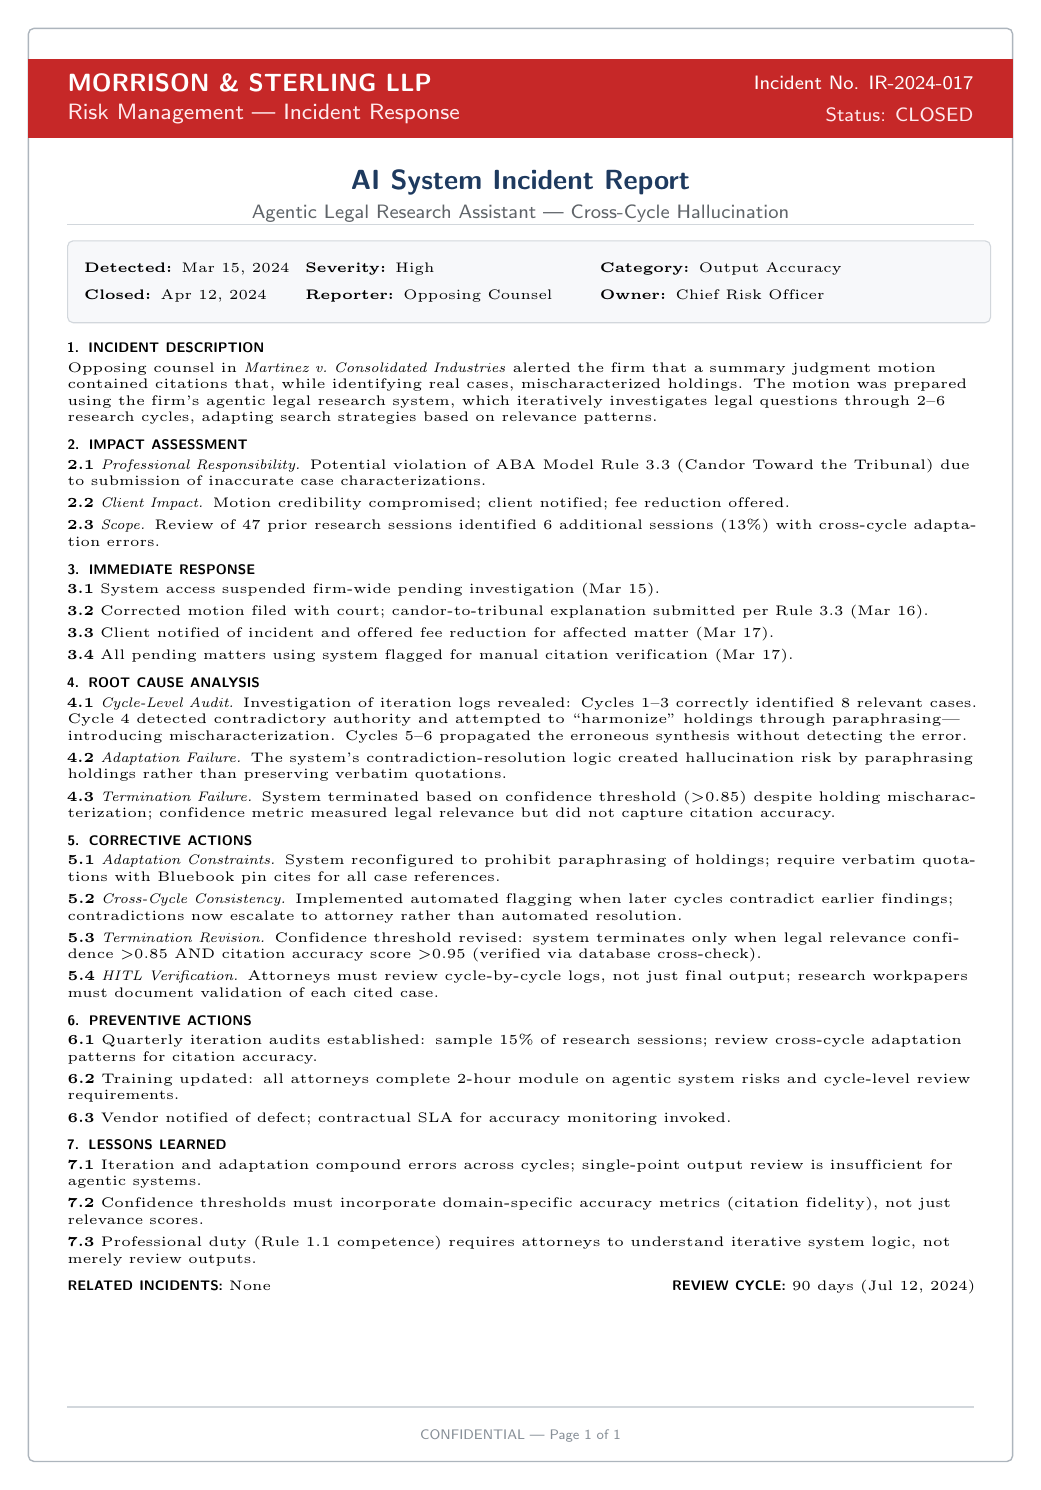
\begin{tikzpicture}[
    every node/.style={inner sep=0pt}
]

% Document frame
\node[
    draw=gray-400,
    line width=0.5pt,
    fill=white,
    minimum width=12.5cm,
    minimum height=18.2cm,
    rounded corners=2pt
] (page) at (0,0) {};

% Header bar
\fill[red-900] ([yshift=-0.4cm]page.north west) rectangle ([yshift=-1.4cm]page.north east);

% Firm name and report title
\node[font=\small\bfseries\sffamily, text=white, anchor=west] at ([xshift=0.5cm, yshift=-0.7cm]page.north west) {MORRISON \& STERLING LLP};
\node[font=\footnotesize\sffamily, text=red-100, anchor=west] at ([xshift=0.5cm, yshift=-1.1cm]page.north west) {Risk Management --- Incident Response};

% Report metadata right side
\node[font=\scriptsize\sffamily, text=white, anchor=east] at ([xshift=-0.5cm, yshift=-0.7cm]page.north east) {Incident No. IR-2024-017};
\node[font=\scriptsize\sffamily, text=red-100, anchor=east] at ([xshift=-0.5cm, yshift=-1.1cm]page.north east) {Status: CLOSED};

% Report title
\node[font=\normalsize\bfseries\sffamily, text=slate-900, anchor=north] at ([yshift=-1.8cm]page.north) {AI System Incident Report};
\node[font=\scriptsize\sffamily, text=gray-600, anchor=north] at ([yshift=-2.25cm]page.north) {Agentic Legal Research Assistant --- Cross-Cycle Hallucination};

% Horizontal rule
\draw[gray-300, line width=0.5pt] ([xshift=0.5cm, yshift=-2.5cm]page.north west) -- ([xshift=-0.5cm, yshift=-2.5cm]page.north east);

% Document metadata box
\node[
    draw=gray-300,
    line width=0.4pt,
    fill=gray-100,
    rounded corners=2pt,
    text width=11.3cm,
    anchor=north west,
    inner sep=6pt,
    font=\tiny
] at ([xshift=0.5cm, yshift=-2.7cm]page.north west) {
\begin{tabular}{@{}l@{\hspace{0.2cm}}l@{\hspace{0.6cm}}l@{\hspace{0.2cm}}l@{\hspace{0.6cm}}l@{\hspace{0.2cm}}l@{}}
\textbf{Detected:} Mar 15, 2024 & \textbf{Severity:} High & \textbf{Category:} Output Accuracy \\[2pt]
\textbf{Closed:} Apr 12, 2024 & \textbf{Reporter:} Opposing Counsel & \textbf{Owner:} Chief Risk Officer \\
\end{tabular}
};

% Report content
\node[
    text width=11.5cm,
    anchor=north west,
    font=\tiny,
    align=left
] at ([xshift=0.5cm, yshift=-4.0cm]page.north west) {
\textbf{\textsf{1. INCIDENT DESCRIPTION}}\\[1pt]
Opposing counsel in \textit{Martinez v.\ Consolidated Industries} alerted the firm that a summary judgment motion contained citations that, while identifying real cases, mischaracterized holdings. The motion was prepared using the firm's agentic legal research system, which iteratively investigates legal questions through 2--6 research cycles, adapting search strategies based on relevance patterns.\\[4pt]

\textbf{\textsf{2. IMPACT ASSESSMENT}}\\[1pt]
\textbf{2.1} \textit{Professional Responsibility.} Potential violation of ABA Model Rule 3.3 (Candor Toward the Tribunal) due to submission of inaccurate case characterizations.\\[2pt]
\textbf{2.2} \textit{Client Impact.} Motion credibility compromised; client notified; fee reduction offered.\\[2pt]
\textbf{2.3} \textit{Scope.} Review of 47 prior research sessions identified 6 additional sessions (13\%) with cross-cycle adaptation errors.\\[4pt]

\textbf{\textsf{3. IMMEDIATE RESPONSE}}\\[1pt]
\textbf{3.1} System access suspended firm-wide pending investigation (Mar 15).\\[2pt]
\textbf{3.2} Corrected motion filed with court; candor-to-tribunal explanation submitted per Rule 3.3 (Mar 16).\\[2pt]
\textbf{3.3} Client notified of incident and offered fee reduction for affected matter (Mar 17).\\[2pt]
\textbf{3.4} All pending matters using system flagged for manual citation verification (Mar 17).\\[4pt]

\textbf{\textsf{4. ROOT CAUSE ANALYSIS}}\\[1pt]
\textbf{4.1} \textit{Cycle-Level Audit.} Investigation of iteration logs revealed: Cycles 1--3 correctly identified 8 relevant cases. Cycle 4 detected contradictory authority and attempted to ``harmonize'' holdings through paraphrasing---introducing mischaracterization. Cycles 5--6 propagated the erroneous synthesis without detecting the error.\\[2pt]
\textbf{4.2} \textit{Adaptation Failure.} The system's contradiction-resolution logic created hallucination risk by paraphrasing holdings rather than preserving verbatim quotations.\\[2pt]
\textbf{4.3} \textit{Termination Failure.} System terminated based on confidence threshold (>0.85) despite holding mischaracterization; confidence metric measured legal relevance but did not capture citation accuracy.\\[4pt]

\textbf{\textsf{5. CORRECTIVE ACTIONS}}\\[1pt]
\textbf{5.1} \textit{Adaptation Constraints.} System reconfigured to prohibit paraphrasing of holdings; require verbatim quotations with Bluebook pin cites for all case references.\\[2pt]
\textbf{5.2} \textit{Cross-Cycle Consistency.} Implemented automated flagging when later cycles contradict earlier findings; contradictions now escalate to attorney rather than automated resolution.\\[2pt]
\textbf{5.3} \textit{Termination Revision.} Confidence threshold revised: system terminates only when legal relevance confidence >0.85 AND citation accuracy score >0.95 (verified via database cross-check).\\[2pt]
\textbf{5.4} \textit{HITL Verification.} Attorneys must review cycle-by-cycle logs, not just final output; research workpapers must document validation of each cited case.\\[4pt]

\textbf{\textsf{6. PREVENTIVE ACTIONS}}\\[1pt]
\textbf{6.1} Quarterly iteration audits established: sample 15\% of research sessions; review cross-cycle adaptation patterns for citation accuracy.\\[2pt]
\textbf{6.2} Training updated: all attorneys complete 2-hour module on agentic system risks and cycle-level review requirements.\\[2pt]
\textbf{6.3} Vendor notified of defect; contractual SLA for accuracy monitoring invoked.\\[4pt]

\textbf{\textsf{7. LESSONS LEARNED}}\\[1pt]
\textbf{7.1} Iteration and adaptation compound errors across cycles; single-point output review is insufficient for agentic systems.\\[2pt]
\textbf{7.2} Confidence thresholds must incorporate domain-specific accuracy metrics (citation fidelity), not just relevance scores.\\[2pt]
\textbf{7.3} Professional duty (Rule 1.1 competence) requires attorneys to understand iterative system logic, not merely review outputs.\\[4pt]

\textbf{\textsf{RELATED INCIDENTS:}} None \hfill \textbf{\textsf{REVIEW CYCLE:}} 90 days (Jul 12, 2024)
};

% Footer
\draw[gray-300, line width=0.5pt] ([xshift=0.5cm, yshift=0.7cm]page.south west) -- ([xshift=-0.5cm, yshift=0.7cm]page.south east);
\node[font=\tiny\sffamily, text=gray-500, anchor=south] at ([yshift=0.25cm]page.south) {CONFIDENTIAL --- Page 1 of 1};

\end{tikzpicture}
\caption{Incident report for an agentic legal research system failure. The report follows ISO 27001 incident management standards (classification, root cause analysis, corrective and preventive actions) while documenting an agentic-specific failure mode: cross-cycle error propagation where the system's adaptation logic introduced hallucinations that compounded across subsequent iterations.}
\label{fig:agents3-incident-report-legal}
\end{figure}


\subsection{Accounting Domain: Independence and Professional Skepticism}
\label{sec:agents3-examples-accounting}

\paragraph{Example 2: AI Acceptable Use Policy for Agentic Systems (AICPA Independence)}
A Big Four accounting firm establishes an AI acceptable use policy to operationalize AICPA independence rules and SEC auditor independence requirements for \emph{agentic audit and advisory systems}. \textit{Dimensional profile: Spans HITL, HOTL, and HIC modes across human and institutional frames; policy-level governance rather than a single system.}

Figure~\ref{fig:agents3-ai-acceptable-use-policy} shows an excerpt from the firm's policy. The policy establishes guiding principles (independence, competence, confidentiality), distinguishes permitted uses (research, analytics, documentation assistance) from prohibited uses (management decisions, audit opinions, unauthorized data sharing), and implements safeguards through vendor approval requirements, mandatory professional review, and documentation standards. Training requirements ensure personnel understand both tool capabilities and professional obligations. Incident reporting procedures establish clear escalation pathways when independence concerns or data breaches arise.

% AI Acceptable Use Policy - Styled as Firm Policy Document (ISO 27001 Compliant)

\begin{figure}[htbp]
\centering
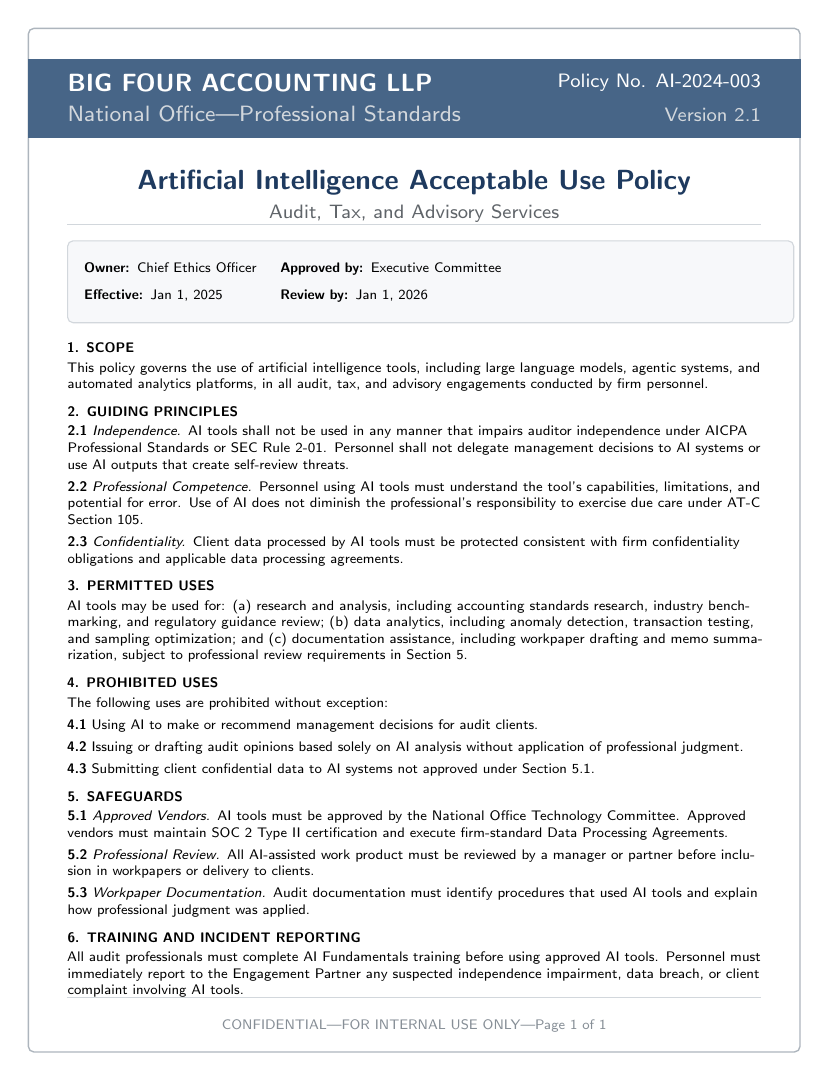
\begin{tikzpicture}[
    every node/.style={inner sep=0pt}
]

% Document frame
\node[
    draw=gray-400,
    line width=0.5pt,
    fill=white,
    minimum width=9.8cm,
    minimum height=13.0cm,
    rounded corners=2pt
] (page) at (0,0) {};

% Header bar
\fill[slate-700] ([yshift=-0.4cm]page.north west) rectangle ([yshift=-1.4cm]page.north east);

% Firm name and policy title
\node[font=\small\bfseries\sffamily, text=white, anchor=west] at ([xshift=0.5cm, yshift=-0.7cm]page.north west) {BIG FOUR ACCOUNTING LLP};
\node[font=\footnotesize\sffamily, text=gray-300, anchor=west] at ([xshift=0.5cm, yshift=-1.1cm]page.north west) {National Office---Professional Standards};

% Policy metadata right side
\node[font=\scriptsize\sffamily, text=white, anchor=east] at ([xshift=-0.5cm, yshift=-0.7cm]page.north east) {Policy No. AI-2024-003};
\node[font=\scriptsize\sffamily, text=gray-300, anchor=east] at ([xshift=-0.5cm, yshift=-1.1cm]page.north east) {Version 2.1};

% Policy title
\node[font=\normalsize\bfseries\sffamily, text=slate-900, anchor=north] at ([yshift=-1.8cm]page.north) {Artificial Intelligence Acceptable Use Policy};
\node[font=\scriptsize\sffamily, text=gray-600, anchor=north] at ([yshift=-2.25cm]page.north) {Audit, Tax, and Advisory Services};

% Horizontal rule
\draw[gray-300, line width=0.5pt] ([xshift=0.5cm, yshift=-2.5cm]page.north west) -- ([xshift=-0.5cm, yshift=-2.5cm]page.north east);

% Document metadata box
\node[
    draw=gray-300,
    line width=0.4pt,
    fill=gray-100,
    rounded corners=2pt,
    text width=8.8cm,
    anchor=north west,
    inner sep=6pt,
    font=\tiny\sffamily
] at ([xshift=0.5cm, yshift=-2.7cm]page.north west) {
\begin{tabular}{@{}l@{\hspace{0.3cm}}l@{\hspace{1.2cm}}l@{\hspace{0.3cm}}l@{}}
\textbf{Owner:} Chief Ethics Officer & \textbf{Approved by:} Executive Committee \\[2pt]
\textbf{Effective:} Jan 1, 2025 & \textbf{Review by:} Jan 1, 2026 \\
\end{tabular}
};

% Policy content - using a single node with formatted text
\node[
    text width=8.8cm,
    anchor=north west,
    font=\tiny\sffamily,
    align=left
] at ([xshift=0.5cm, yshift=-4.0cm]page.north west) {
\textbf{\textsf{1. SCOPE}}\\[1pt]
This policy governs the use of artificial intelligence tools, including large language models, agentic systems, and automated analytics platforms, in all audit, tax, and advisory engagements conducted by firm personnel.\\[4pt]

\textbf{\textsf{2. GUIDING PRINCIPLES}}\\[1pt]
\textbf{2.1} \textit{Independence.} AI tools shall not be used in any manner that impairs auditor independence under AICPA Professional Standards or SEC Rule 2-01. Personnel shall not delegate management decisions to AI systems or use AI outputs that create self-review threats.\\[2pt]
\textbf{2.2} \textit{Professional Competence.} Personnel using AI tools must understand the tool's capabilities, limitations, and potential for error. Use of AI does not diminish the professional's responsibility to exercise due care under AT-C Section 105.\\[2pt]
\textbf{2.3} \textit{Confidentiality.} Client data processed by AI tools must be protected consistent with firm confidentiality obligations and applicable data processing agreements.\\[4pt]

\textbf{\textsf{3. PERMITTED USES}}\\[1pt]
AI tools may be used for: (a) research and analysis, including accounting standards research, industry benchmarking, and regulatory guidance review; (b) data analytics, including anomaly detection, transaction testing, and sampling optimization; and (c) documentation assistance, including workpaper drafting and memo summarization, subject to professional review requirements in Section 5.\\[4pt]

\textbf{\textsf{4. PROHIBITED USES}}\\[1pt]
The following uses are prohibited without exception:\\[2pt]
\textbf{4.1} Using AI to make or recommend management decisions for audit clients.\\[2pt]
\textbf{4.2} Issuing or drafting audit opinions based solely on AI analysis without application of professional judgment.\\[2pt]
\textbf{4.3} Submitting client confidential data to AI systems not approved under Section 5.1.\\[4pt]

\textbf{\textsf{5. SAFEGUARDS}}\\[1pt]
\textbf{5.1} \textit{Approved Vendors.} AI tools must be approved by the National Office Technology Committee. Approved vendors must maintain SOC 2 Type II certification and execute firm-standard Data Processing Agreements.\\[2pt]
\textbf{5.2} \textit{Professional Review.} All AI-assisted work product must be reviewed by a manager or partner before inclusion in workpapers or delivery to clients.\\[2pt]
\textbf{5.3} \textit{Workpaper Documentation.} Audit documentation must identify procedures that used AI tools and explain how professional judgment was applied.\\[4pt]

\textbf{\textsf{6. TRAINING AND INCIDENT REPORTING}}\\[1pt]
All audit professionals must complete AI Fundamentals training before using approved AI tools. Personnel must immediately report to the Engagement Partner any suspected independence impairment, data breach, or client complaint involving AI tools.
};

% Footer
\draw[gray-300, line width=0.5pt] ([xshift=0.5cm, yshift=0.7cm]page.south west) -- ([xshift=-0.5cm, yshift=0.7cm]page.south east);
\node[font=\tiny\sffamily, text=gray-500, anchor=south] at ([yshift=0.25cm]page.south) {CONFIDENTIAL---FOR INTERNAL USE ONLY---Page 1 of 1};

\end{tikzpicture}
\caption{AI acceptable use policy excerpt operationalizing AICPA and SEC independence requirements for professional services firms.}
\label{fig:agents3-ai-acceptable-use-policy}
\end{figure}


\textbf{Governance Principles Demonstrated}:
\begin{itemize}
\item \textbf{Domain-specific calibration}: Policy tailored to AICPA and SEC independence rules, not generic AI governance.
\item \textbf{Role-based permissions}: Distinguishes permitted (research, analytics) from prohibited (management decisions, audit opinions) uses.
\item \textbf{Accountability assignment}: Partners responsible for reviewing AI-assisted work; National Office Ethics Group accountable for policy updates.
\end{itemize}



% Section 7: Conclusion (Synthesis and Path Forward)
% ============================================================================
% 08-conclusion.tex
% Conclusion
% Part of: Chapter 07 - Agents Part II: How to Build an Agent
% ============================================================================

\section{Conclusion}
\label{sec:agents2-conclusion}

We began with a simple claim: AI agents are organized like professional teams. The associate reviewing a credit agreement needs tools (Westlaw, the precedent database), memory (prior deals, client context), planning (decompose the review into sections), protocols (how to communicate findings), and evaluation (partner review of work product). The portfolio manager monitoring client mandates needs the same components in a different domain: tools (Bloomberg, the risk engine), memory (investment research, client history), planning (coordinate monitoring, rebalancing, compliance, and risk agents), protocols (how agents share tasks and artifacts), and evaluation (continuous performance monitoring).

The reference architectures in Section~\ref{sec:agents2-synthesis} made this concrete. The credit facility review agent used ReAct planning to work through document sections, MCP tools to access precedent databases and legal research, episodic memory to track findings within the transaction, and three-layer evaluation to measure retrieval accuracy, analysis quality, and workflow completion. The portfolio management system used hierarchical planning to coordinate specialist agents, A2A protocol for task delegation and artifact exchange, and continuous evaluation to ensure mandate compliance.

But we were also honest about limitations. Current agents achieve under 10\% success on tasks exceeding four hours. Compounding errors, hallucinations in agentic loops, and brittleness at integration boundaries mean these reference architectures represent target states, not current reality. Production deployment requires human oversight, decomposition into shorter tasks, and acceptance that agents accelerate work rather than replace professional judgment.

\paragraph{What You Now Understand}

You understand that \textbf{tools} give agents the ability to interact with systems---accessing databases, running calculations, generating documents. Without tools, an agent is just a chatbot. With tools, it becomes capable of real work.

You understand that \textbf{memory} enables agents to maintain context and learn from experience---case files, precedent databases, client histories, investment research. Without memory, every interaction starts from scratch.

You understand that \textbf{planning} allows agents to decompose complex goals into manageable steps---ReAct for exploration, Plan-Execute for systematic coverage, hierarchical coordination for multi-agent workflows.

You understand that \textbf{protocols} govern how agents access tools and collaborate---MCP for standardized tool integration, A2A for agent-to-agent coordination. Protocol choice determines interoperability and audit capability.

You understand that \textbf{evaluation} measures whether agents perform at professional standards---retrieval accuracy, reasoning quality, workflow completion, security compliance. Generic benchmarks are insufficient; you need domain-specific metrics and expert review.

\paragraph{What This Lets You Do}

You can evaluate vendor claims critically. Is their ``agentic AI'' really autonomous, or just prompt engineering? Does the architecture support your workflows? What tools, memory, and planning capabilities does it actually have?

You can participate in procurement by asking the right questions. You can design governance that maps controls to architectural components. You can communicate with technical teams because you understand the system architecture. You can design deployment strategies that match your organization's risk tolerance.

\begin{keybox}[title={Architecture Enables Governance}]
You cannot govern what you do not understand. Now that you understand how agents work---their tools, memory, planning, protocols, and evaluation---you are ready to establish controls, set policies, assign accountability, and ensure compliance.
\end{keybox}

% ----------------------------------------------------------------------------
% Governance Bridge
% ----------------------------------------------------------------------------

\subsection{From Architecture to Governance}
\label{sec:agents2-governance-bridge}

Production systems in legal and financial contexts operate under governance obligations that transform architectural components into compliance artifacts. Every tool invocation becomes an audit log entry. Every memory write becomes a data retention decision subject to the tensions we examined---auditability without over-collection, structured logging without indefinite raw trace retention. Every planning step becomes a decision record subject to regulatory review.

When an SEC examiner reviews a compliance monitoring agent that detected a mandate breach, they will ask: When did the system detect the problem? What data supported the conclusion? Who approved the corrective action? What controls prevented the agent from exceeding its authority? These questions map directly to architectural components: event timestamps, tool invocation logs, memory retrieval records, and authorization checks.

Similarly, when a legal research agent accesses privileged materials, every access must respect privilege boundaries. An agent that crosses matter boundaries creates waiver risk comparable to an associate who emails the wrong client's confidential materials. The memory system's isolation controls and access logs become evidence in privilege disputes.

The architectural components you now understand become governance objects. Tools become objects of authorization policies---and the security mitigations we examined (prompt injection defense, tool result validation, privilege escalation prevention) become compliance requirements. Memory becomes subject to retention policies, legal hold obligations, and the tiered retention architecture that balances auditability with data minimization. Planning becomes subject to oversight mechanisms specifying which decisions require human review. Protocols become the infrastructure for authentication, logging, and audit trails. Evaluation becomes assurance processes that verify controls operate as intended.

\begin{keybox}[title={The Governance Imperative}]
Part III addresses a fundamental principle: \textbf{professional duties are non-delegable}. When an attorney files a brief, they are responsible for its accuracy---regardless of whether AI assisted in drafting it. When an investment adviser recommends a strategy, they bear fiduciary duty---regardless of whether an agent generated the analysis. When an auditor signs an opinion, they vouch for its conclusions---regardless of the tools used to reach them.

``The AI did it'' is not a defense to malpractice, breach of fiduciary duty, or professional sanctions.

The architecture in this chapter enables professionals to meet those non-delegable duties. The audit trails support accountability. The human-in-the-loop gates preserve professional judgment. The termination conditions prevent unbounded autonomous action. The security controls protect confidentiality. But architecture alone is insufficient---you must also establish policies, assign responsibilities, and ensure ongoing compliance.

Part III provides that governance framework. It maps the GPA+IAT properties to specific controls, establishes dimensional calibration for risk-based oversight, and translates principles into operational practice. The architecture you now understand makes governance possible. Part III makes it real.
\end{keybox}



% ============================================================================
% BIBLIOGRAPHY
% ============================================================================
\printbibliography

\end{document}
